\documentclass[titlepage]{WARPdoc}
\usepackage{graphicx}
\usepackage{color}

\begin{document}

\title{Platform Support Package: sysgen2opb}
\author{Elliot Ng}
\organization{Rice University WARP Project\\ Center for Multimedia Communication\\ \href{http://warp.rice.edu/}{http://warp.rice.edu/}}
\version{1.3}
\maketitle

\tableofcontents





\section{Introduction}
sysgen2opb is one of several tools in the Platform Support Package for the Rice University Wireless Open-Access Research Platform (WARP). sysgen2opb is a Matlab script which converts a Xilinx System Generator (Sysgen) model into an OPB-compliant peripheral for use with embedded PowerPCs or other OPB bus masters. The result can be integrated within Xilinx Platform Studio (XPS).\\ \\ The sysgen2opb script replaces each System Generator Gateway In and Gateway Out with a memory mapped I/O register, accessible over the OPB. It also creates the necessary address decode logic and a C header file with the resulting register map. This functionality allows software to write/read data to/from the I/O ports of the synthesized System Generator model.  Alternatively, if an addressable dual-port storage block is used within a Sysgen model, the storage element may be mapped directly into the OPB memory space, obviating the need for a separate address bridge register between the OPB and the storage element.  This functionality, termed the shared memory extension, permits higher throughput when accessing shared storage elements. \\ \\ In summary, there are three ways in which the opb2sysgen script can be utilized.

\begin{enumerate}
	\item Simple Script - This script simply maps Sysgen gateways into software-accessible registers.  It supports versions 7.1 and 8.1 of Xilinx System Generator.
	\item Shared Memory Extension Script - This script is identical to the simple script, with an additional shared memory extension. Shared memory support requires the use of dual port RAMs, and may be used only with version 8.1 of Xilinx System Generator.
	\item Configurable Subsystem Extension Script - This script is identical to the simple script, with an additional configurable subsystem extension. It will take the gateways and registers and store them in a library of configurable subsystems. This script is to be used only with version 8.1 of Xilinx System Generator.
\end{enumerate}





\newpage
\section{General Design Flow}
This section briefly describes the design flow for producing an OPB-compliant core from a Sysgen model. It is assumed herein that the reader is familiar with Matlab, Simulink, System Generator, and Xilinx Platform Studio.
\begin{enumerate}
	\item Select a directory in which your system generator model will reside.  The complete path name of this working directory must not contain any spaces.
	\item Build a System Generator model of the peripheral core which will later be converted into your OPB-compliant peripheral.
	\item Copy the Matlab script file \textit{sysgen2opb.m} and the peripheral model file \\\textit{skeleton\_periph\_model.mdl} to the same directory as the model being converted.
	\item Execute \textit{sysgen2opb.m} to convert the model.
	\item Use Sysgen to generate your peripheral core from the converted model.  If you already have an existing XPS project in which the peripheral core will be used, System Generator may be configured to copy the generated core into the project's local user repository.  Otherwise, the generated core may be placed in any other user-specified directory.
	\item If you do not have an existing XPS project, create one.
	\item If necessary, copy the newly generated peripheral core into your XPS project's local user repository.
	\item Add the peripheral core to your XPS project and verify/update the system address map.  In XPS, the address range spanned by the peripheral (from base address to high address) MUST match the address range defined at the time of conversion! If it is necessary to remap the core to a different address range, the core must be regenerated from the original unconverted model.
	\item Write any user software required to interact with the peripheral core.
	\item Compile the complete system.
	\item Download and test the system.
\end{enumerate}





\newpage
\section{Rules/Requirements}
\subsection{General Requirements}
\begin{enumerate}
	\item The script file sysgen2opb.m and skeleton peripheral model skeleton\_periph\_model.mdl must reside in the same directory as the model to be converted.
	\item The script requires that at least one Gateway In and one Gateway Out will be converted into memory-mapped registers. For cases in which no Gateway In or no Gateway Out is required, a single dummy instance of the missing gateway must be instantiated.
	\item The base address must be 32 bits in width.
	\item The complete path name of the working directory (the one containing the model to be converted) must not contain any spaces.  The directory My Documents, for example, is not valid in the working directory path. 
	\item Any Boolean type connected to a Gateway Out that will be converted to a register must be cast to a UFix1\_0. 
	\item A maximum of 450 combined input and output gateways may be converted to registers.
	\item All gateways that will become registers must be clocked at the system sample period.
	\item The path to each output gateway must contain a synchronous element.
\end{enumerate}

\subsection{Simple Script with Shared Memory Extension}
	\subsubsection{General Requirements}
		\begin{enumerate}
			\item OPB address [19:16] determines whether the lower order 16 address bits (spanning 64 KBytes) access memory mapped registers or shared memory blocks. The first 64 KBytes, starting at the peripheral's base address, are reserved for memory mapped registers. Each subsequent 64 KByte memory region is reserved for an individual shared memory block. Consider, for example, a peripheral with a base address of 0xFF010000. Addresses 0xFF010000 through 0xFF01FFFF access simple memory mapped registers.  Addresses 0xFF02000 \\through 0xFF02FFFF access the first shared memory block. Addresses 0xFF03000 through 0xFF03FFFF access the second shared memory block, and so on.
			\item The maximum number of shared memory blocks equals (15 - bin2dec(base address [19:16])). If base address is 0xFF000000, one register region and up to 15 shared memories are allowed. If base address is 0xFF010000, one register region and up to 14 shared memories are allowed.  If base address is 0xFF0F0000, only one register region is allowed (no shared memories).
			\item The shared memory extension is defined to function only with dual-port RAM blocks.

				\begin{figure}[htbp]
					\centering
					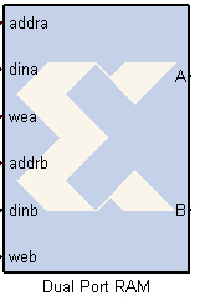
\includegraphics[width=0.10\textwidth]{scriptimages/dpram.pdf}
					\caption{Dual Port RAM}
					\label{fig:dpram}
				\end{figure}
			\item Port "A" of the Dual Port RAM is user-defined
			\item Port "B" of the Dual Port RAM has additional requirements, described below. 
		\end{enumerate}
	\subsubsection{DPRAM (Read-Only) Requirements}
		\begin{enumerate}
			\item DPRAM Name Prefix: SMRO\_
			\item Source block for DPRAM addrb input
			
			\begin{enumerate}
				\item Name Prefix: SMROAddr\_
				\item Block Type: Gateway In
				\item Output Type: UFix14\_0			
			\end{enumerate}
		
			\item Source block for DPRAM dinb input
			\begin{enumerate}
				\item Name Prefix: SMRODataI\_
				\item Block Type: Xilinx Constant
				\item Constant Value: 0
				\item Number of bits: 32
			\end{enumerate}
		
			\item Source block for DPRAM web input
			
			\begin{enumerate}
				\item Name Prefix: SMROWE\_
				\item Block Type: Xilinx Constant
				\item Output Type: Boolean
				\item Constant Value: 0
			\end{enumerate}
		
			\item Destination block for DPRAM B output
		
			\begin{itemize}
				\item Name Prefix: SMRODataO\_
				\item Block Type: Gateway Out
			\end{itemize}
	
			\item The figure below illustrates a valid implementation of a dual-port RAM whose B port will be mapped into the OPB memory space using the read only shared memory extension.  Note that the A port is user-defined, and that the restrictions described herein apply only to the B port.
				\begin{figure}[htbp]
					\centering
					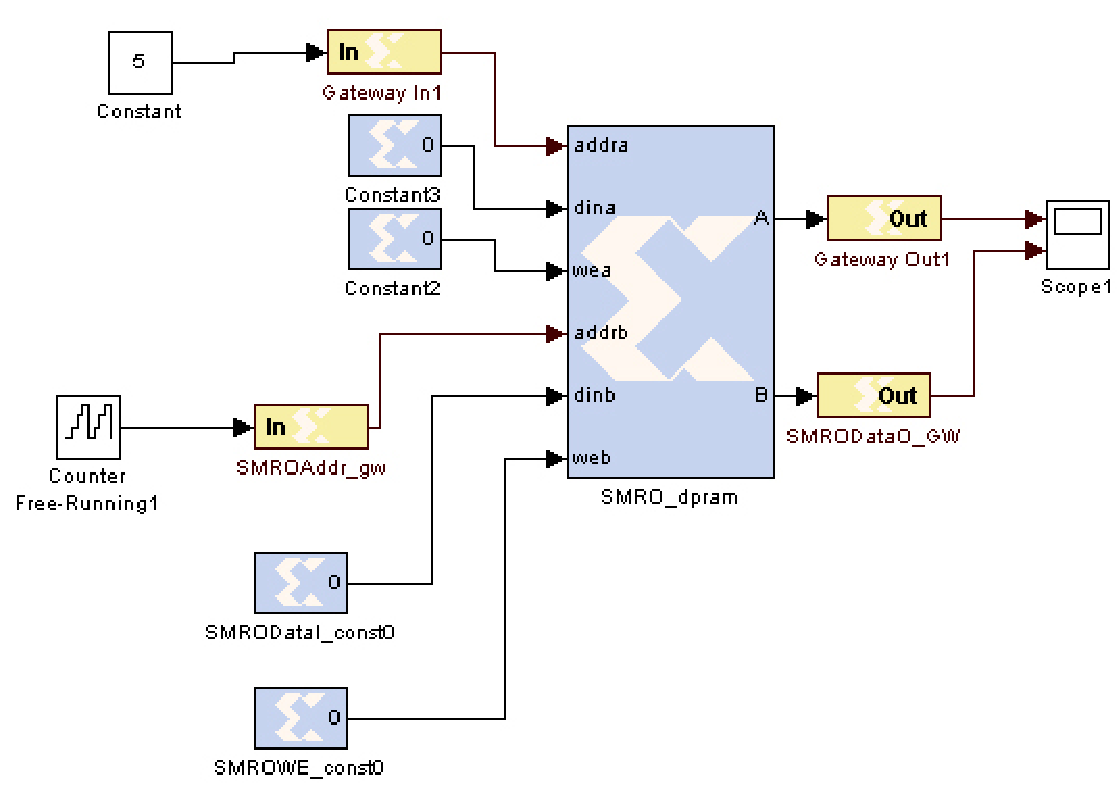
\includegraphics[width=0.60\textwidth]{scriptimages/SMRO_dpram.pdf}
					\caption{Sample Read-only Dual Port RAM Model}
					\label{fig:SMRO_dpram}
				\end{figure}
		\end{enumerate}	
	
	\newpage	
	\subsubsection{DPRAM (Write-Only) Requirements}	
		\begin{enumerate}
			\item DPRAM Name Prefix: SMWO\_
			\item Source block for DPRAM addrb input
	
			\begin{enumerate}
				\item Name Prefix: SMWOAddr\_
				\item Block Type: Gateway In
				\item Output Type: UFix14\_0
			\end{enumerate}
		
			\item Source block for DPRAM dinb input
		
			\begin{enumerate}
				\item Name Prefix: SMWODataI\_
				\item Block Type: Gateway In
				\item Number of bits: 32
			\end{enumerate}
		
			\item Source block for DPRAM web input
						
			\begin{enumerate}
				\item Name Prefix: SMWOWE\_
				\item Block Type: Gateway In
				\item Output Type: Boolean
			\end{enumerate}
		
		\item The figure below illustrates a valid implementation of a dual-port RAM whose B port will be mapped into the OPB memory space using the write only shared memory extension.  Note that the A port is user-defined, and that the restrictions described herein apply only to the B port.

			\begin{figure}[htbp]
				\centering
				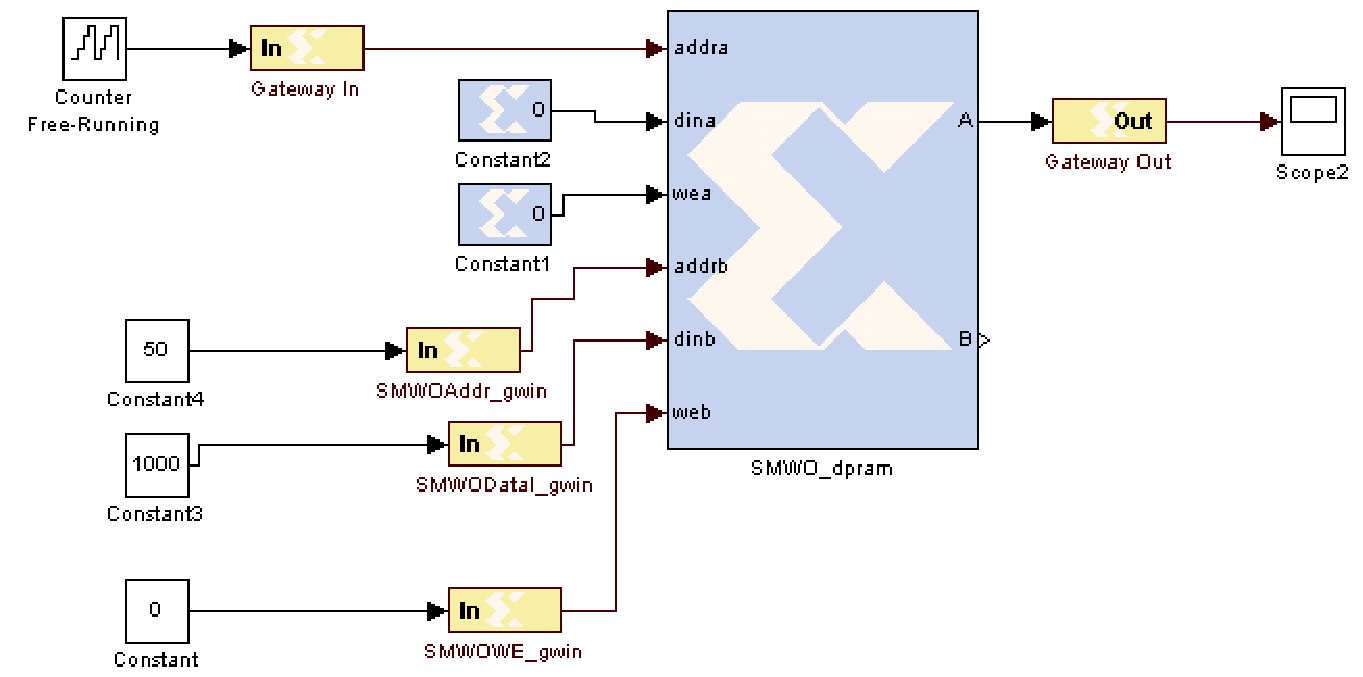
\includegraphics[width=0.60\textwidth]{scriptimages/SMWO_dpram.pdf}
				\caption{Sample Write-only Dual Port RAM Model}
				\label{fig:SWRO_dpram}
			\end{figure}
		\end{enumerate}

\newpage
\section{Example with Simple Registers}

	\subsection{Overview}
	This example illustrates a process by which a System Generator model is converted into an OPB-compliant peripheral core.  When the converted core is later imported into a XPS design, the model's input and output gateways are mapped into software-accessible registers on the OPB.  Data is then moved into and out of the core through writes/reads to/from these software-accessible registers.  An option is also provided to specify that specific gateways will not be mapped into registers.  These ''no\_reg'' gateways are mapped into generic I/O ports in the top level of the converted core, permitting direct connection to other cores or to FPGA pins in the system. 

	\subsection{Software/System Requirements}
	This example uses System Generator version 8.1 and Xilinx Platform Studio (XPS) version 8.1.  More detailed requirements, including restrictions on file and directory names, are discussed in the section titled ''Rules/Requirements''.  It is assumed that the reader is familiar enough with MATLAB, Simulink, and System Generator to create simple Simulink models and execute simple MATLAB scripts. 

	\subsection{Xilinx Platform Studio - Base System Builder}
Create XPS project. Use Base System Builder to build the project. For more information on using Base System Builder, please refer to the WARP document ''FPGA Board User IO Reference Design'' section ''Setting up the Project in XPS.''

	\subsection{Matlab/System Generator}
	\begin{enumerate}
		\item Run Matlab.
		\item Open the Simulink Library Browser.
		\item Expand Xilinx Blockset in the Simulink Library Browser.
		\item Select File $\rightarrow$ New $\rightarrow$ Model from the menu options at the top of the Simulink Library Browser window. 
		\item In the resulting Simulink model window, select File $\rightarrow$ Save As. Type adder in the file name field. Click save.
		\item Drag the following blocks from the Simulink Library Browser to the new Simulink Model:
			\begin{enumerate}
				\item Simulink/Commonly Used Blocks/Scope
				\item Simulink/Sources/Counter Free-Running
				\item Xilinx Blockset/Basic Elements/System Generator
				\item Xilinx Blockset/Basic Elements/Gateway In
				\item Xilinx Blockset/Basic Elements/Gateway In  (the name should default to Gateway In1)
				\item Xilinx Blockset/Basic Elements/Gateway Out
				\item Xilinx Blockset/Math/AddSub 
			\end{enumerate}
		\item Double click on the Counter Free-Running block. Set Number of Bits to 6 and Sample time to 1.
		\item	Double click on the Gateway In block. In the Basic tab, set the Output type to Unsigned, the Number of bits to 6, the Binary point to 0, the Quantization to Round, the Overflow to Saturate, and the Sample period to 1. Press OK. Do the same for Gateway In1. 
		\item Double click on the AddSub block. Under the Basic tab, set Operation to Addition and Latency to 1. Under the Output Type tab, set Precision to Full. Press OK. 
		\item Rename Gateway Out to Sum. 
		\item Double click on the Scope block. Click on Scope parameters (the second button from the left within the toolbar at the top of the Scope display window). Set Number of axes to 3. Click OK. Close the Scope display window. The Scope should now display three input ports. 
		\item Connect the Counter Free-Running block so that it feeds the two input gateways and the top two input ports of the scope.  Connect the output gateway to the bottom input port of the scope. Connect the input and output gateways to the inputs and output of the adder block.  The resulting model should appear as shown below.
			
			\begin{figure}[htbp]
				\centering
				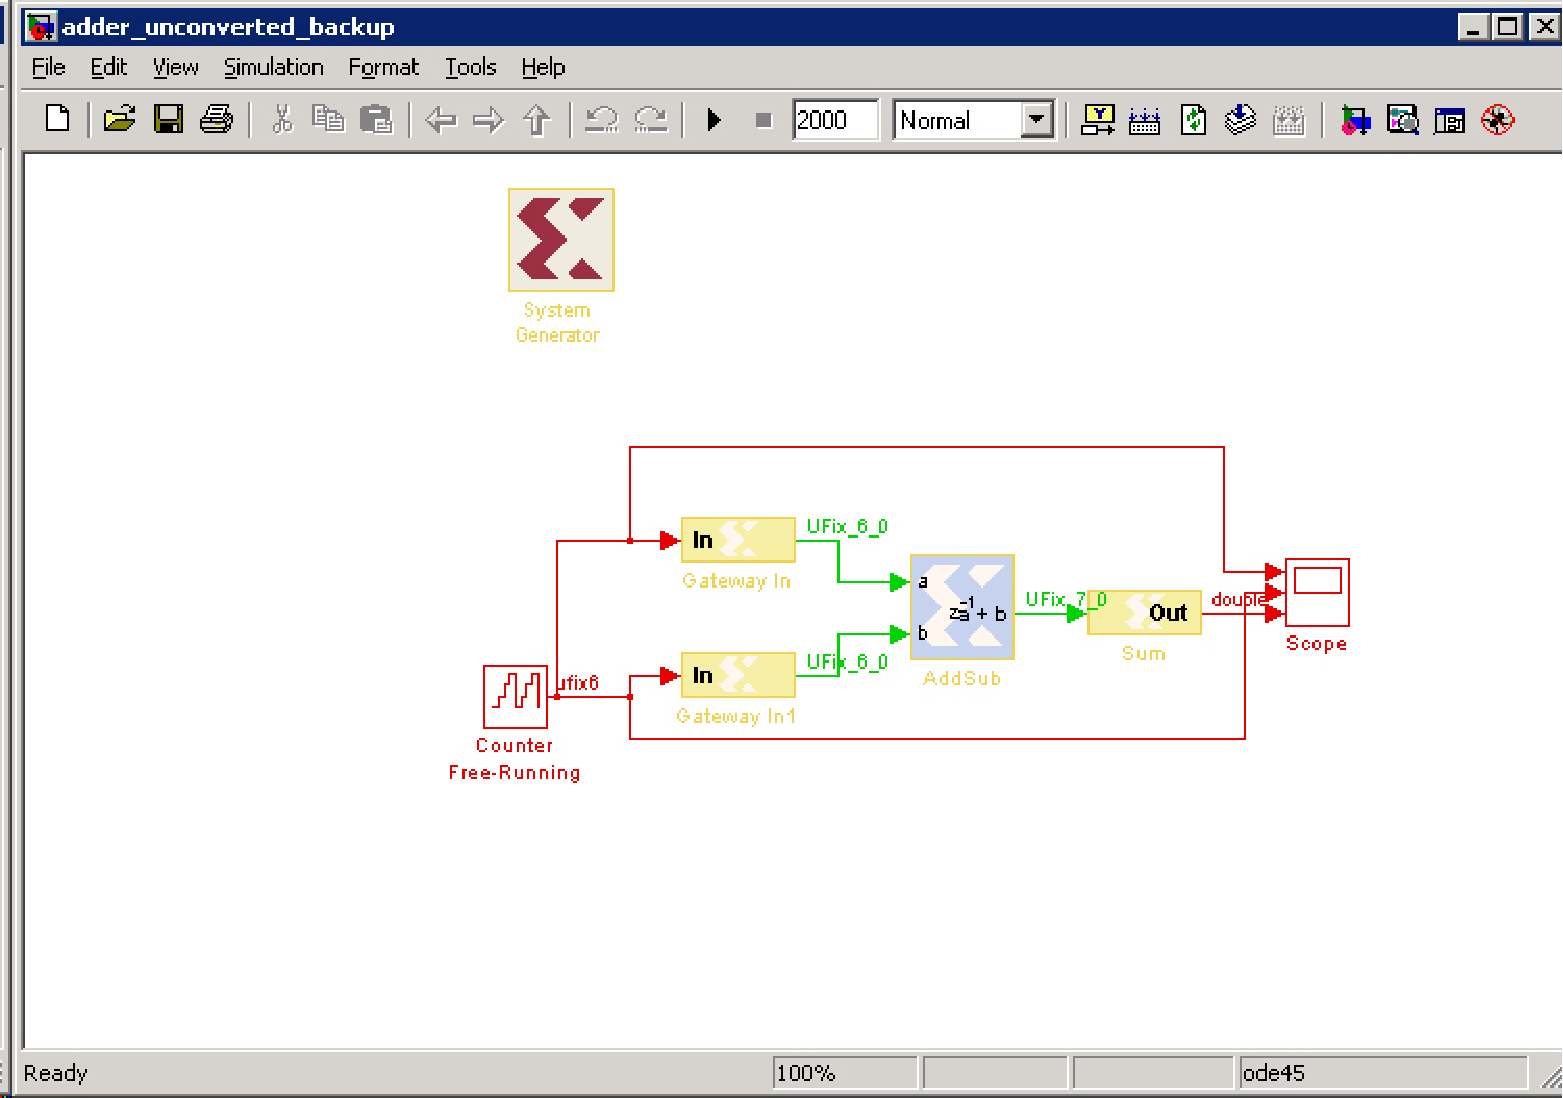
\includegraphics[width=0.70\textwidth]{scriptimages/sysgen1.pdf}
				\caption{Example System Generator Model}
				\label{fig:sysgen1}
			\end{figure}

		\item From the menu bar at the top of the Simulink model window, select Format $\rightarrow$ Port/Signal Displays. Make sure Sample Time Colors, Port Data Types, and Signal Dimensions are selected. 
		\item From the WARP repository, copy sysgen2opb.m and skeleton\_periph\_model.mdl to the directory in which the System Generator model adder.mdl is located.
		\item In the Matlab Command Window, execute \textit{sysgen2opb('adder', hex2dec('FF000000'))}.  This script will close the model window and then convert it to an OPB-compliant peripheral with ports mapped to a range of addresses starting at hexadecimal FF000000.  A copy of the original unconverted model will be saved to the file adder\_unconverted\_backup.mdl.
		\newpage
		\item Reopen adder.mdl to view the converted model.  Note that several blocks may need to be rearranged for aesthetic reasons.		
			
			\begin{figure}[htbp]
				\centering
				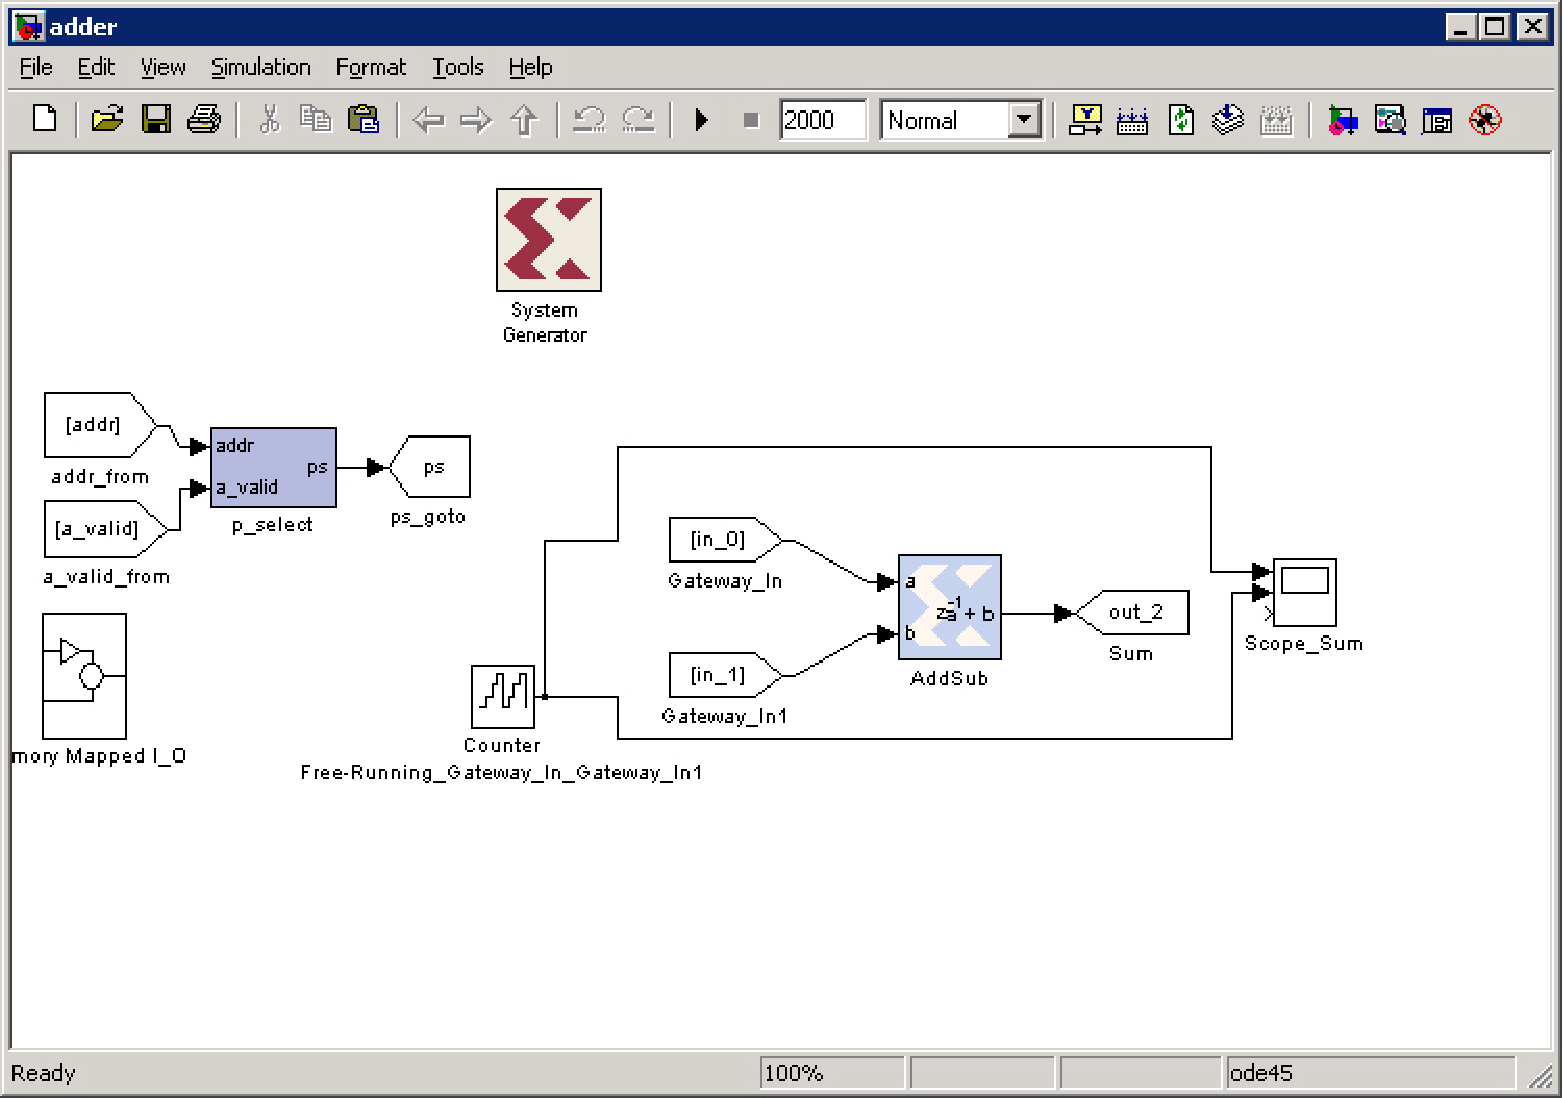
\includegraphics[width=0.70\textwidth]{scriptimages/sysgen2.pdf}
				\caption{Converted System Generator Model}
				\label{fig:sysgen2}
			\end{figure}

		\item Double click on the System Generator block.  A System Generator properties window for the current model will appear.  In this window, set Compilation to OPB Export Tool.  Set Part to Virtex2p xc2vp70-6ff1517.  Set Synthesis Tool to XST.  Set Hardware Description Language to VHDL.  Set FPGA Clock Period (ns) to 20.

			\begin{figure}[htbp]
				\centering
				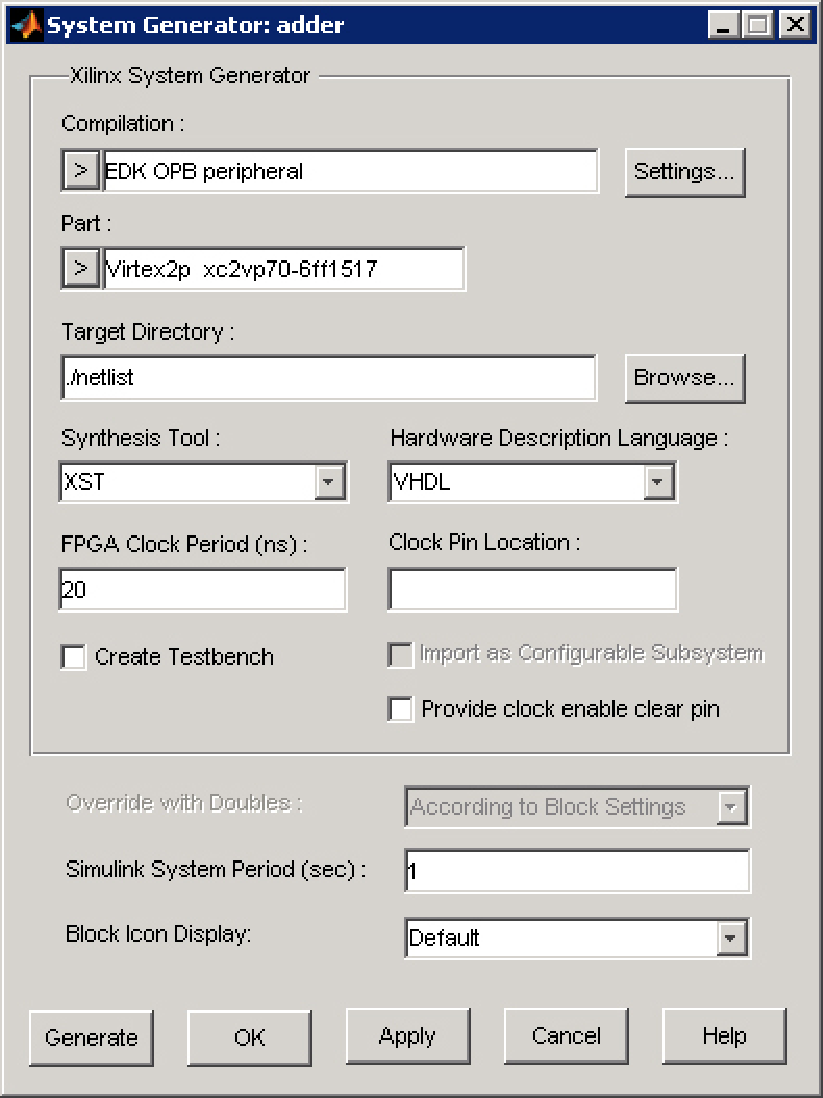
\includegraphics[width=0.30\textwidth]{scriptimages/sysgen3.pdf}
				\caption{System Generator Properties}
				\label{fig:sysgen3}
			\end{figure}

		\item The Target Directory field specifies the location to which output files from the script will be written.  Using the fefault value of ./netlist results in the creation of a directory named netlist within the same directory containing the adder.mdl model.
		\item If you have not yet created an XPS project in which the OPB peripheral will be used, simply click Generate to complete the process of creating the core.  In this scenario, a directory named pcore will be created within the Target Directory.  Within this pcore directory, another directory named adder\_opbw will be created.  Later, this directory (adder\_opbw) may be moved or copied into the core repository of an XPS project for use within that project.
		\item If you do have an existing XPS project, and would like the converted core to be placed within the project's core repository, click Settings at the top right of System Generator Properties window.  Make sure that the Export button is highlighted, then browse for an XPS project file (*.xps).  Once the project file has been selected, click Generate in the System Generator properties window.  A directory named adder\_opbw will be created within the XPS project's local pcore directory, making it available for use within the XPS project.
		
		\begin{figure}[htbp]
			\centering
			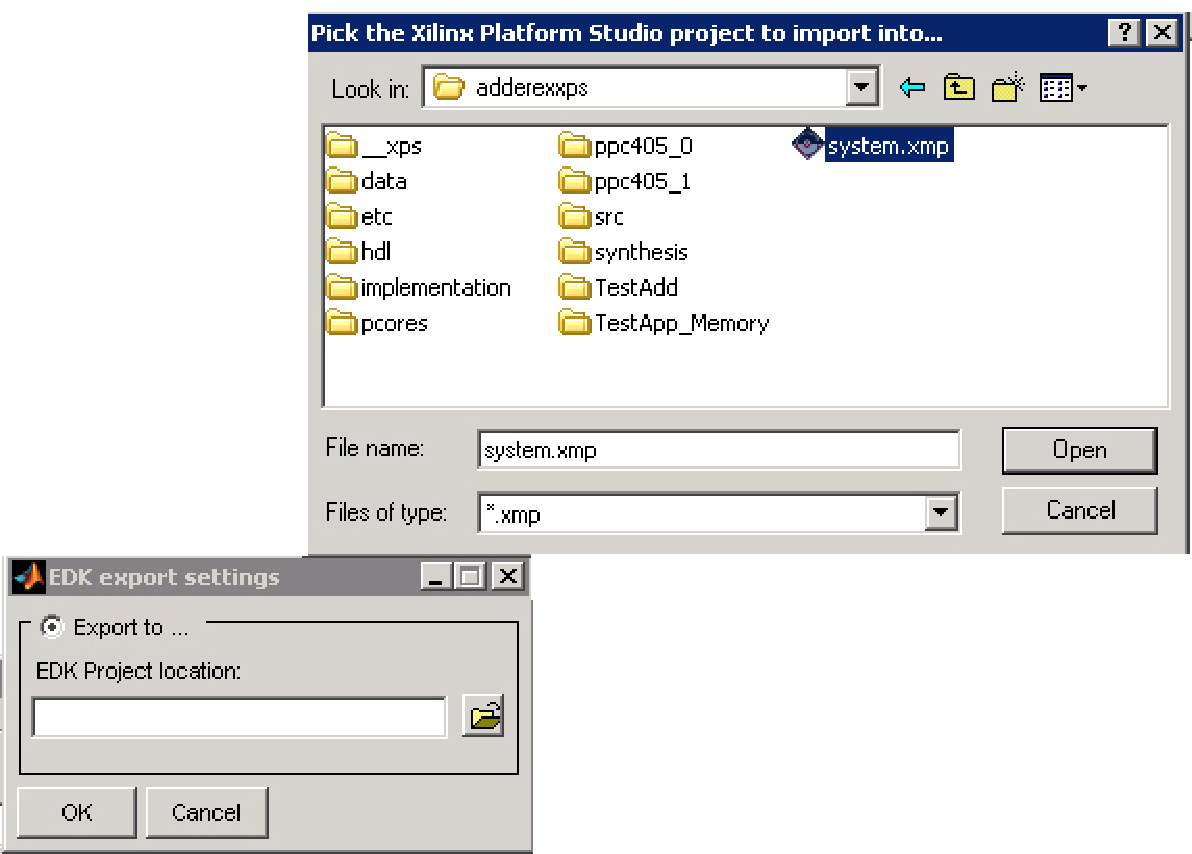
\includegraphics[width=0.50\textwidth]{scriptimages/settings.pdf}
			\caption{EDK Export Settings dialog and Open dialog}
		\end{figure}

		\item At this point, your system generator model has been converted to an OPB-compliant peripheral that may be imported into an existing XPS project.

	\end{enumerate}

	\newpage
	\subsection{Xilinx Platform Studio - Using XPS}
	\begin{enumerate}			
			\item This section assumes that the peripheral core directory produced by System Generator already resides within the local user repository of the XPS project that will utilize the peripheral.  If necessary, copy the directory now.
			\item From the menu options at the top of the XPS main window, click Project $\rightarrow$ Rescan User Repositories.
			
			\item Click on the IP Catalog tab. Expand Project Repository. You should see adder\_opbw listed in Project Repository. Right-click on adder\_opbw and select Add IP. There may be a popup window that asks, ''Are you sure you want to add this IP?'' If so, click Yes.
				\begin{figure}[htbp]
					\centering
					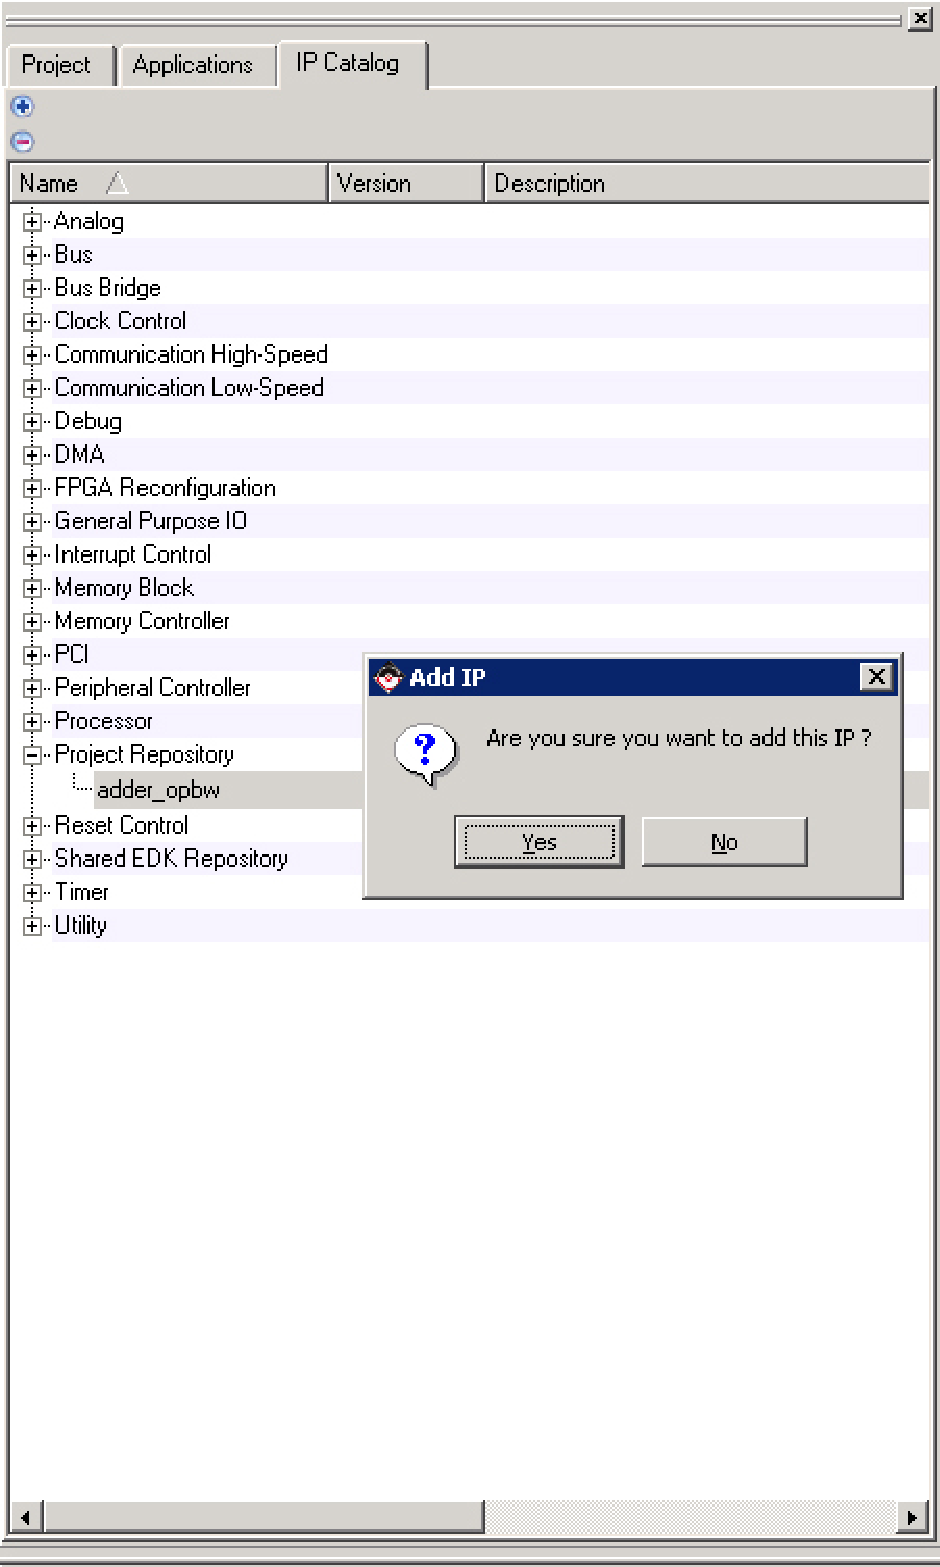
\includegraphics[width=0.30\textwidth]{ORIGdemo/16.pdf}
					\label{fig:16}
				\end{figure}
				\newpage
				
			\item Click on the System Assembly Tab. 
			
			\begin{enumerate}
				\item Select the Bus Interface radio button within Filters. This resulting view illustrates connections between available buses and available peripheral cores.  Click the grayed-out circle located at the intersection of the on-chip peripheral bus (OPB) and peripheral adder\_opbw\_0. This will expand adder\_opbw\_0 to show an underlying SOPB item. Click on the grayed-out circle located at the intersection of OPB and the newly visible SOPB item. This will cause the circle to be filled in, and will result in a connection between the OPB and the peripheral's slave OPB interface. On adder\_opbw\_0 $\rightarrow$ SOPB, you will see that the Bus Connection field lists opb.
					\begin{figure}[htbp]
						\centering
						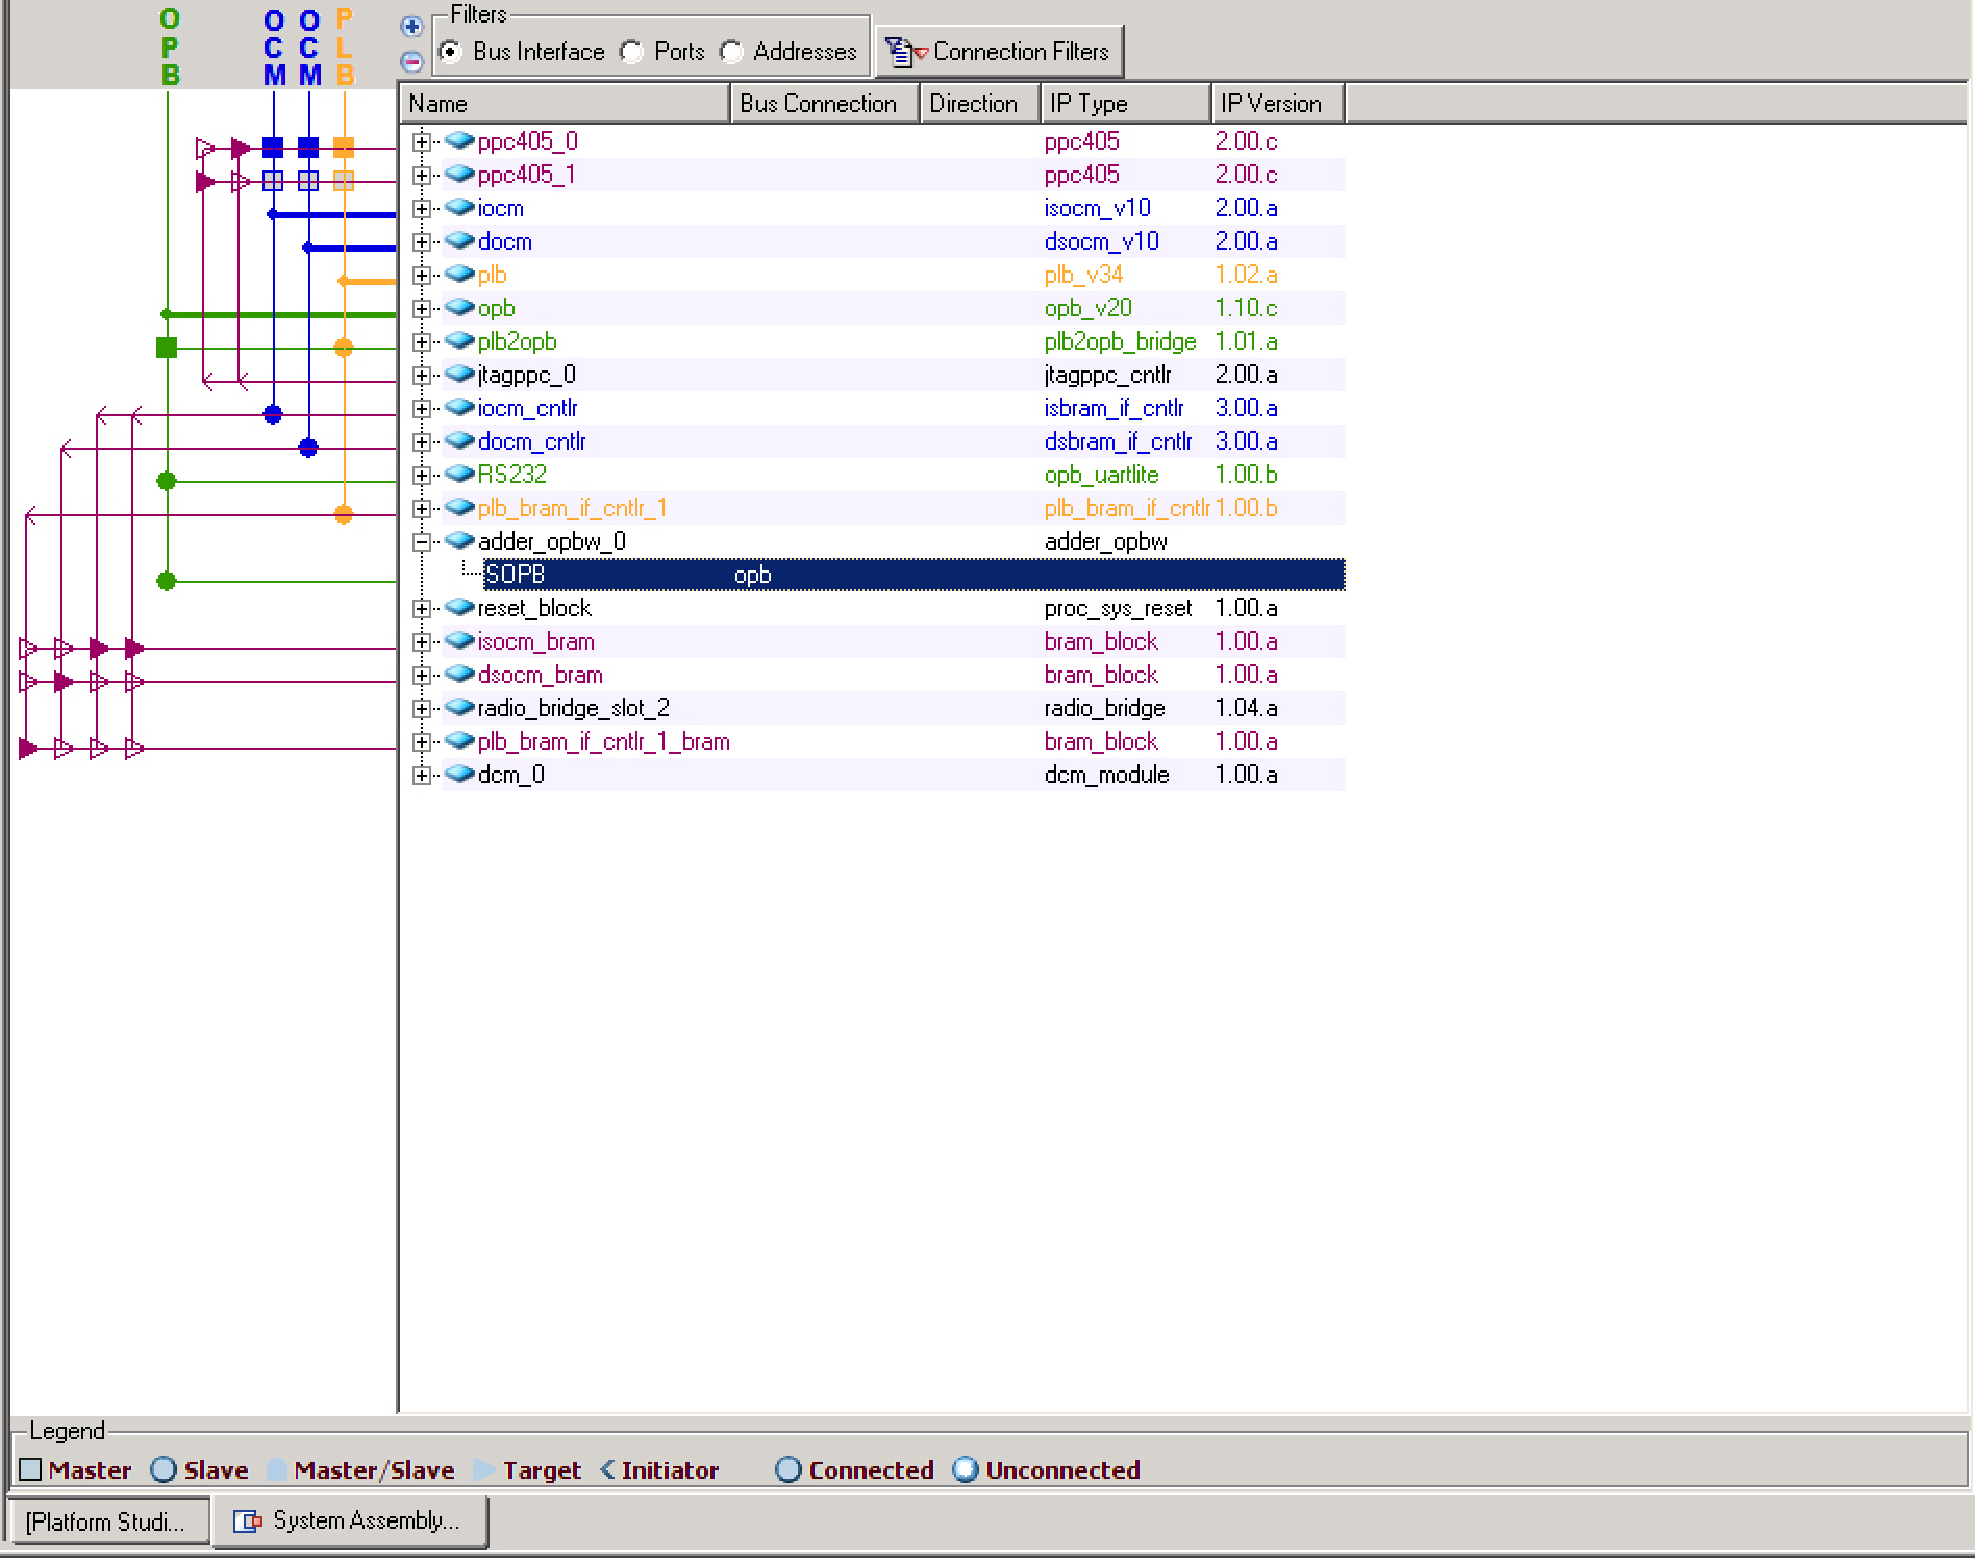
\includegraphics[width=0.70\textwidth]{ORIGdemo/17.pdf}
						\label{fig:17}
					\end{figure}
				\newpage

				\item Select the Ports radio button within Filters. The resulting view illustrates port-to-signal mappings for all peripherals. Expand adder\_opbw\_0. Beneath it, you will find the port name ce. Click within ce port's the Net field. In the resulting drop-down menu, select net\_vcc. This will connect a constant ''1'' to the peripheral's ce input port. Click somewhere else within this window for this connection to take effect.
					\begin{figure}[htbp]
						\centering
						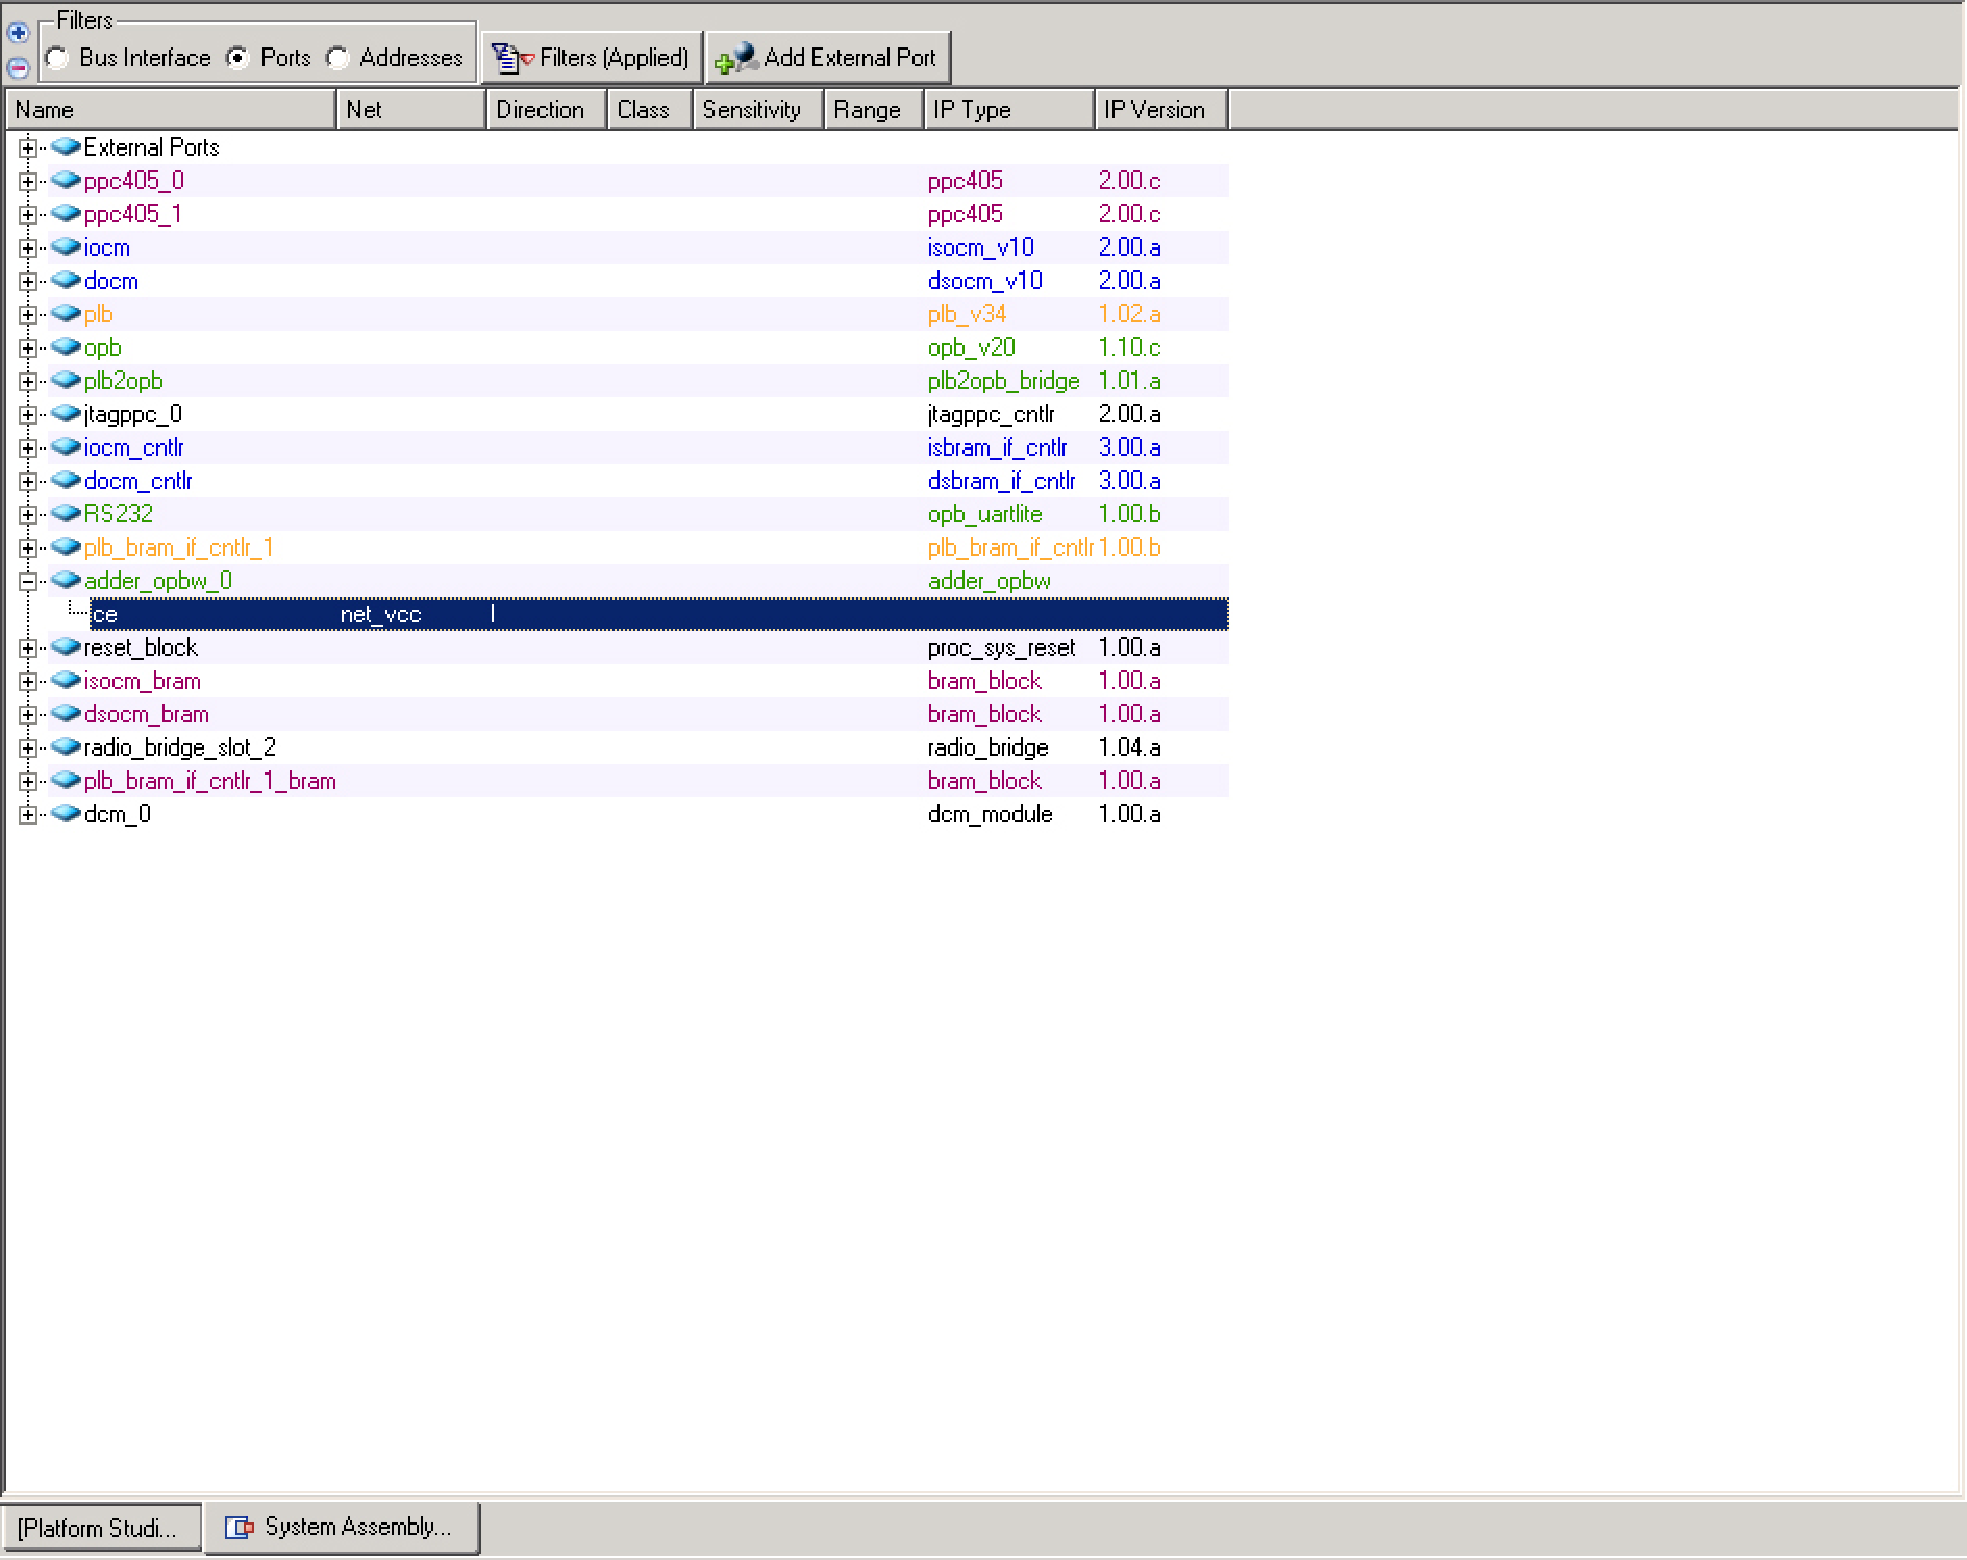
\includegraphics[width=0.70\textwidth]{ORIGdemo/18.pdf}
						\label{fig:18}
					\end{figure}

				\newpage				
				\item Select the Addresses radio button within Filters. The resulting view illustrates address mappings for all peripherals. Click within the Base Address field of peripheral \\adder\_opbw\_0. Set the base address to 0xFF000000. Click somewhere else within this window for the change to be accepted.  If, after clicking somewhere else, the base address appears incorrect, simply reenter a base address of 0xFF000000. Again, click somewhare else within the window for the change to take effect. Click on the Lock box for peripheral adder\_opbw\_0. A check mark should appear in the box. Click somewhare else within the window for the change to take effect, then click Generate Addresses.
					\begin{figure}[htbp]
						\centering
						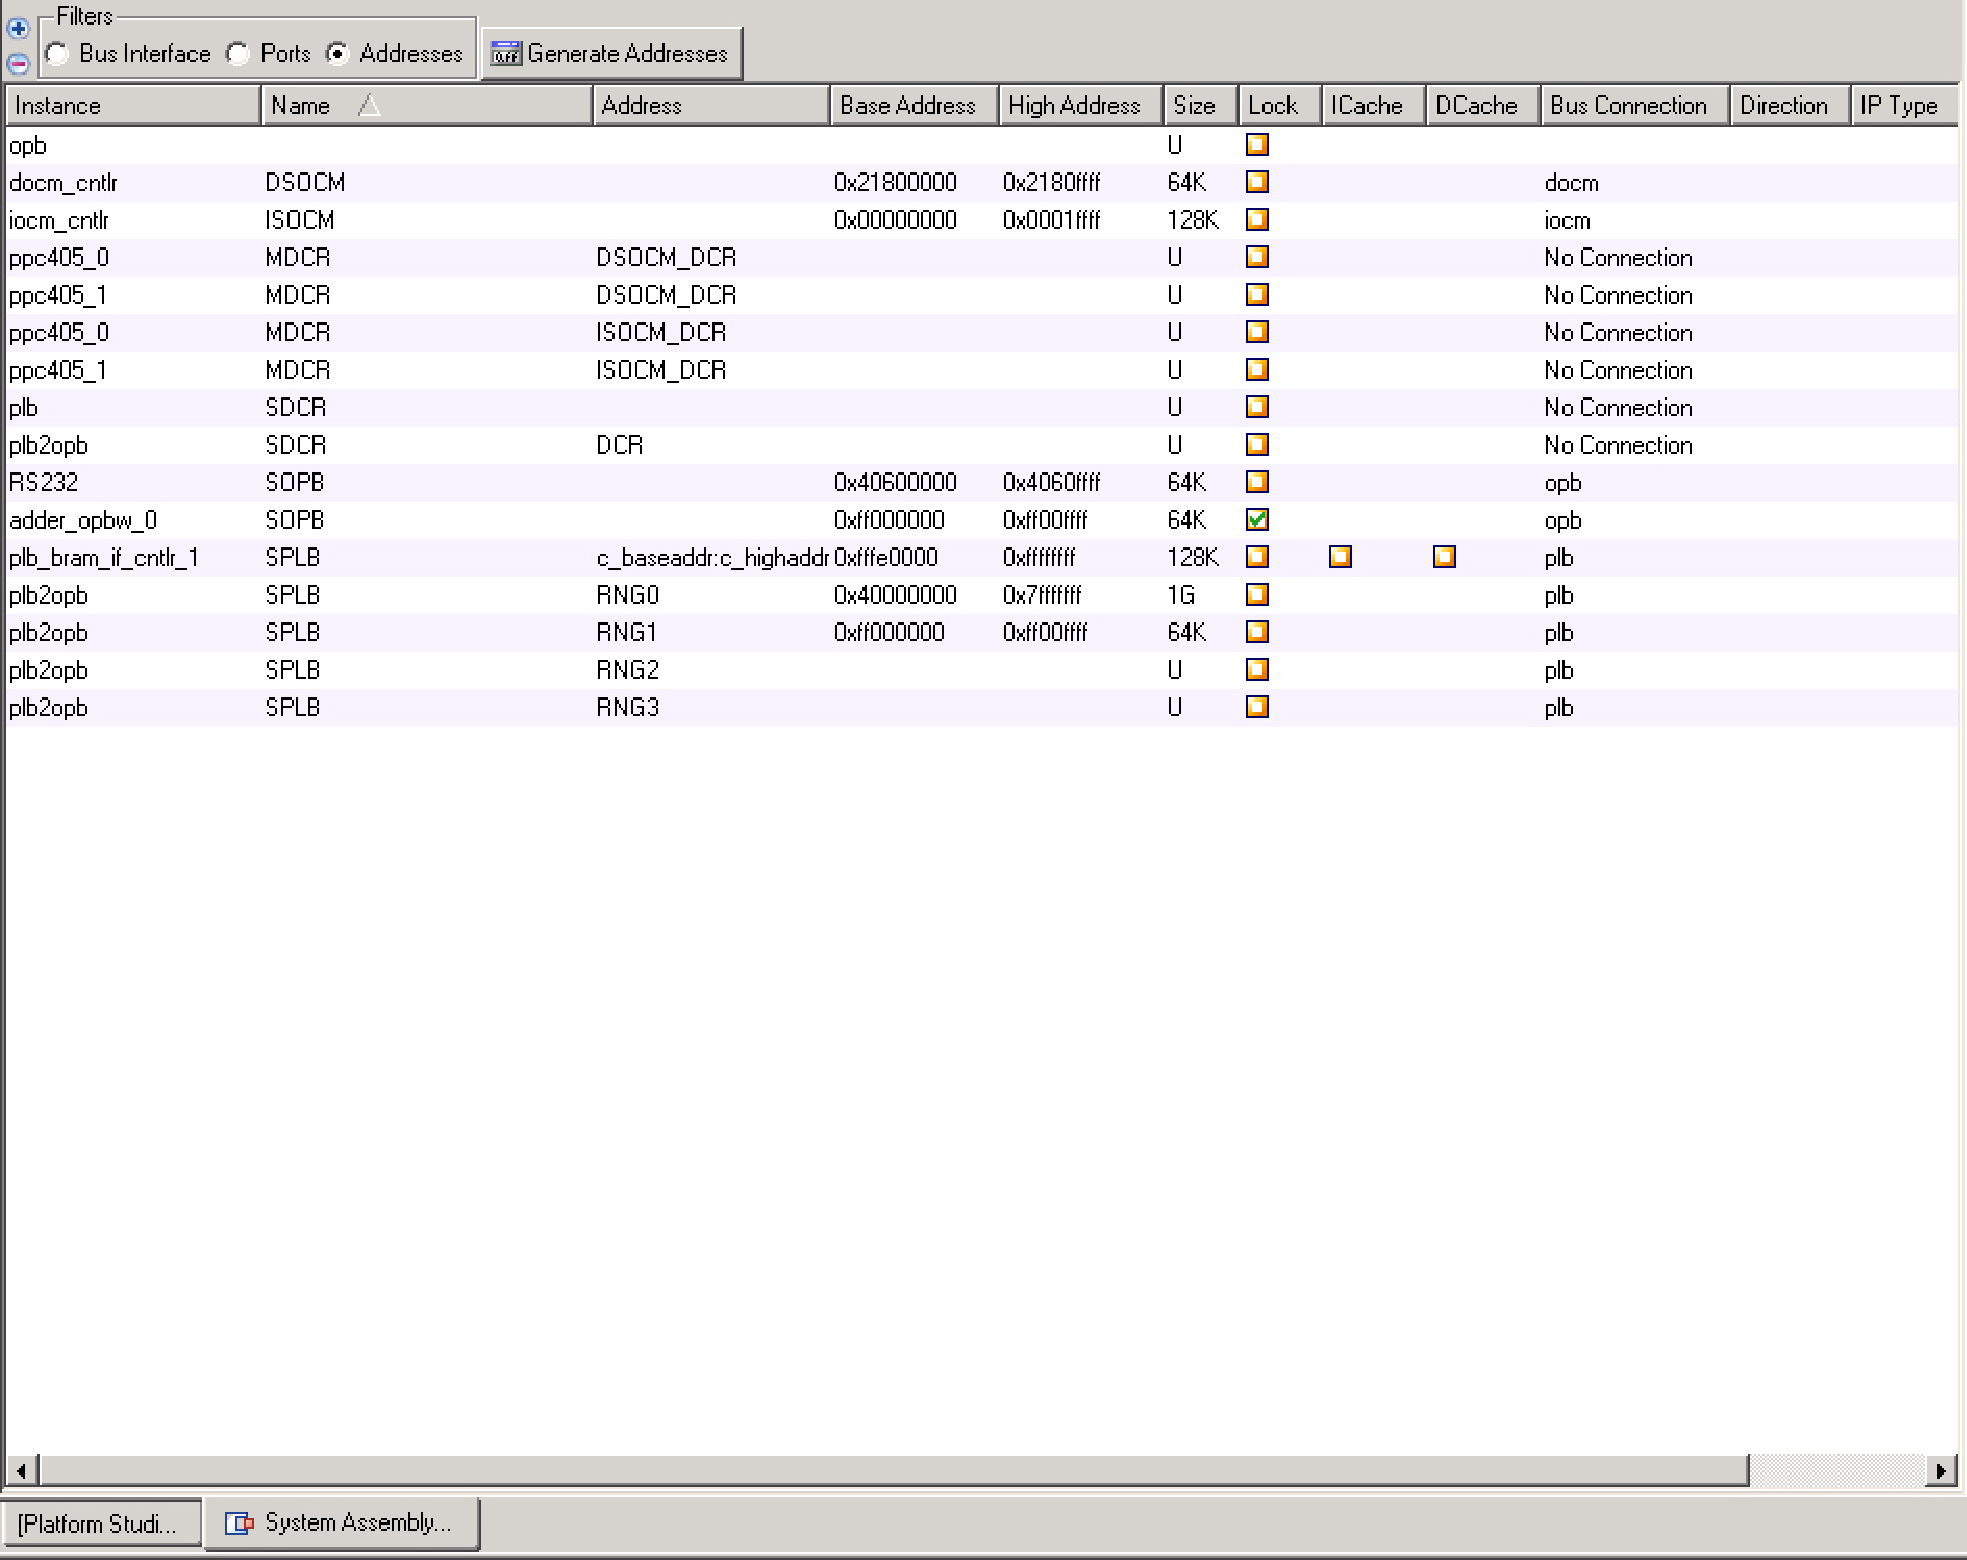
\includegraphics[width=0.70\textwidth]{ORIGdemo/19.pdf}
						\label{fig:19}
					\end{figure}
				
			\end{enumerate}
			
			\newpage
			\item Click on the Applications tab. Right click on Project: TestApp\_Memory and deselect Mark to Initialize Bram. Double-click on Add Software Application Project. Name it TestAdder. Processor should be set to ppc405\_0. Click OK. Right click on Project: TestAdder and select Mark to Initialize BRAM. 
				\begin{figure}[htbp]
					\centering
					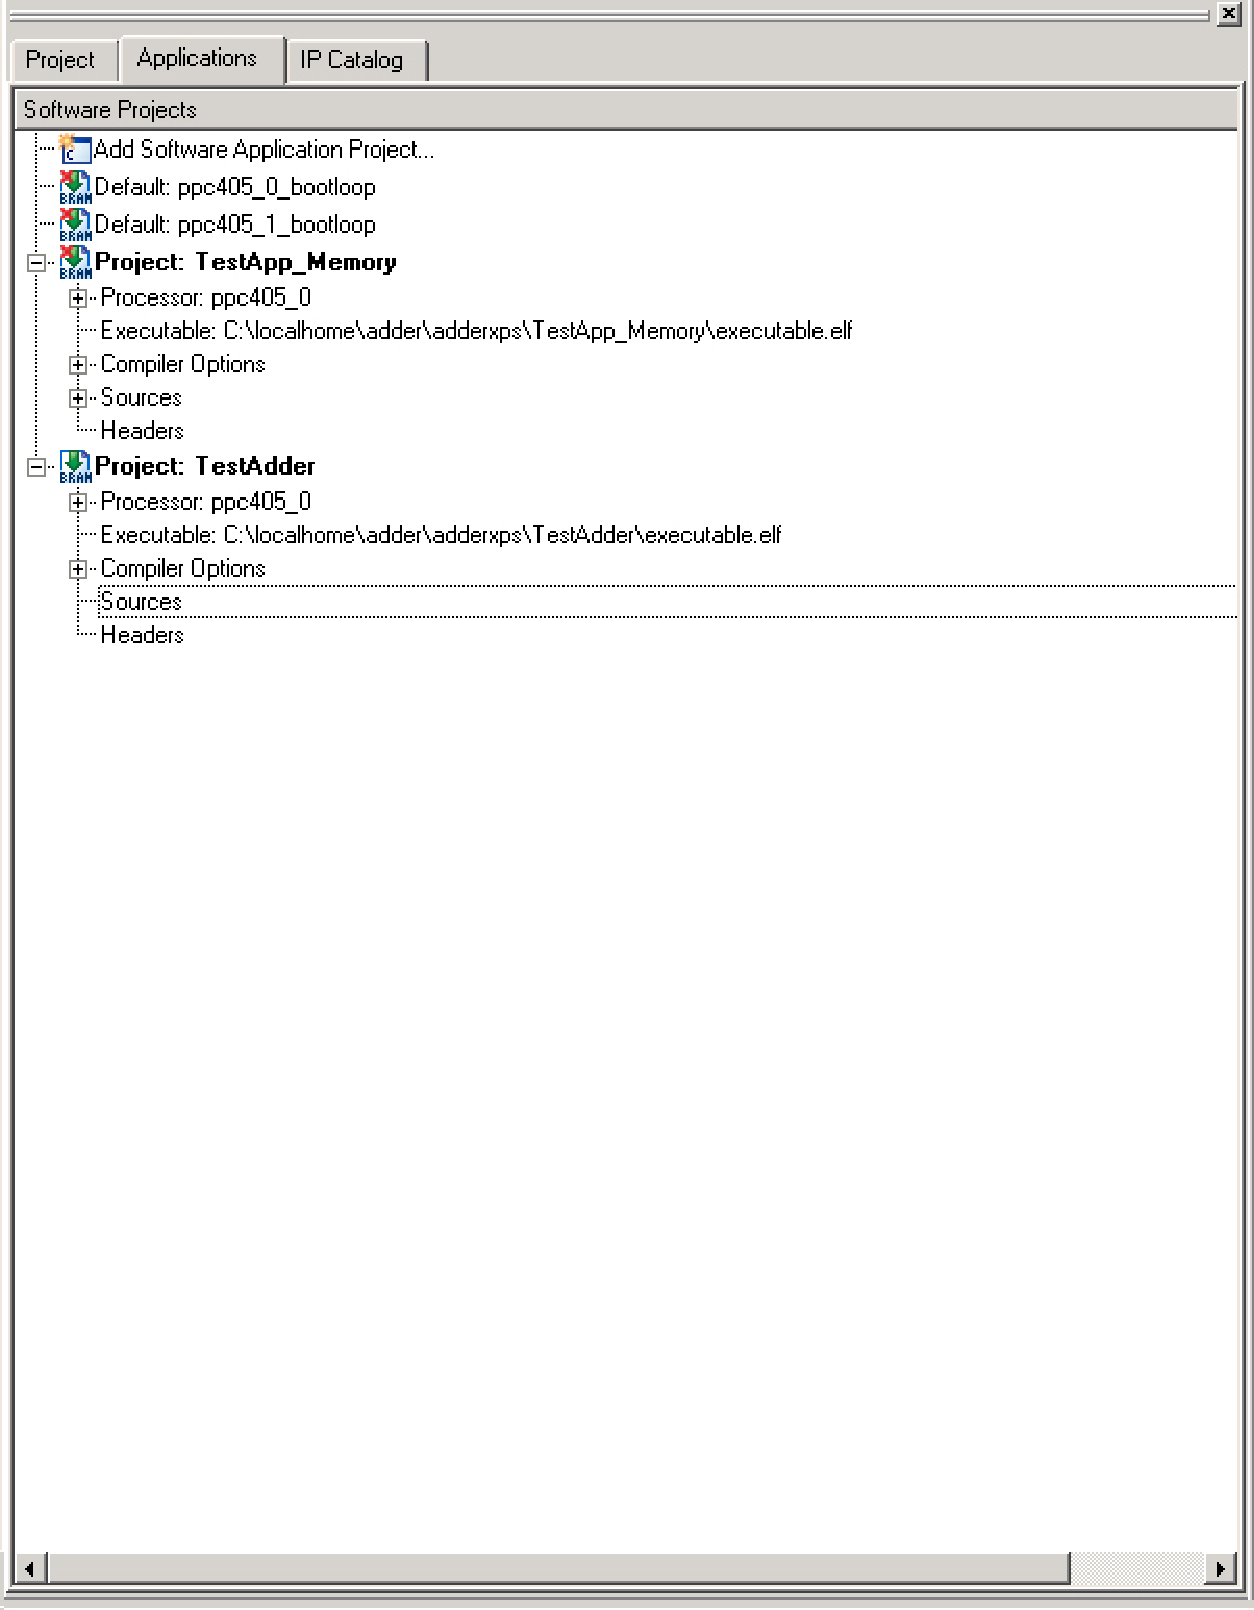
\includegraphics[width=0.40\textwidth]{ORIGdemo/20.pdf}
					\label{fig:20}
				\end{figure}
			
				
			\item Under Project: TestAdder, right-click on Sources. Select Add New File. Create a new folder src. Go to the src folder. Put in the file name TestAdder.c . Click Save. 
				\begin{figure}[htbp]
					\centering
					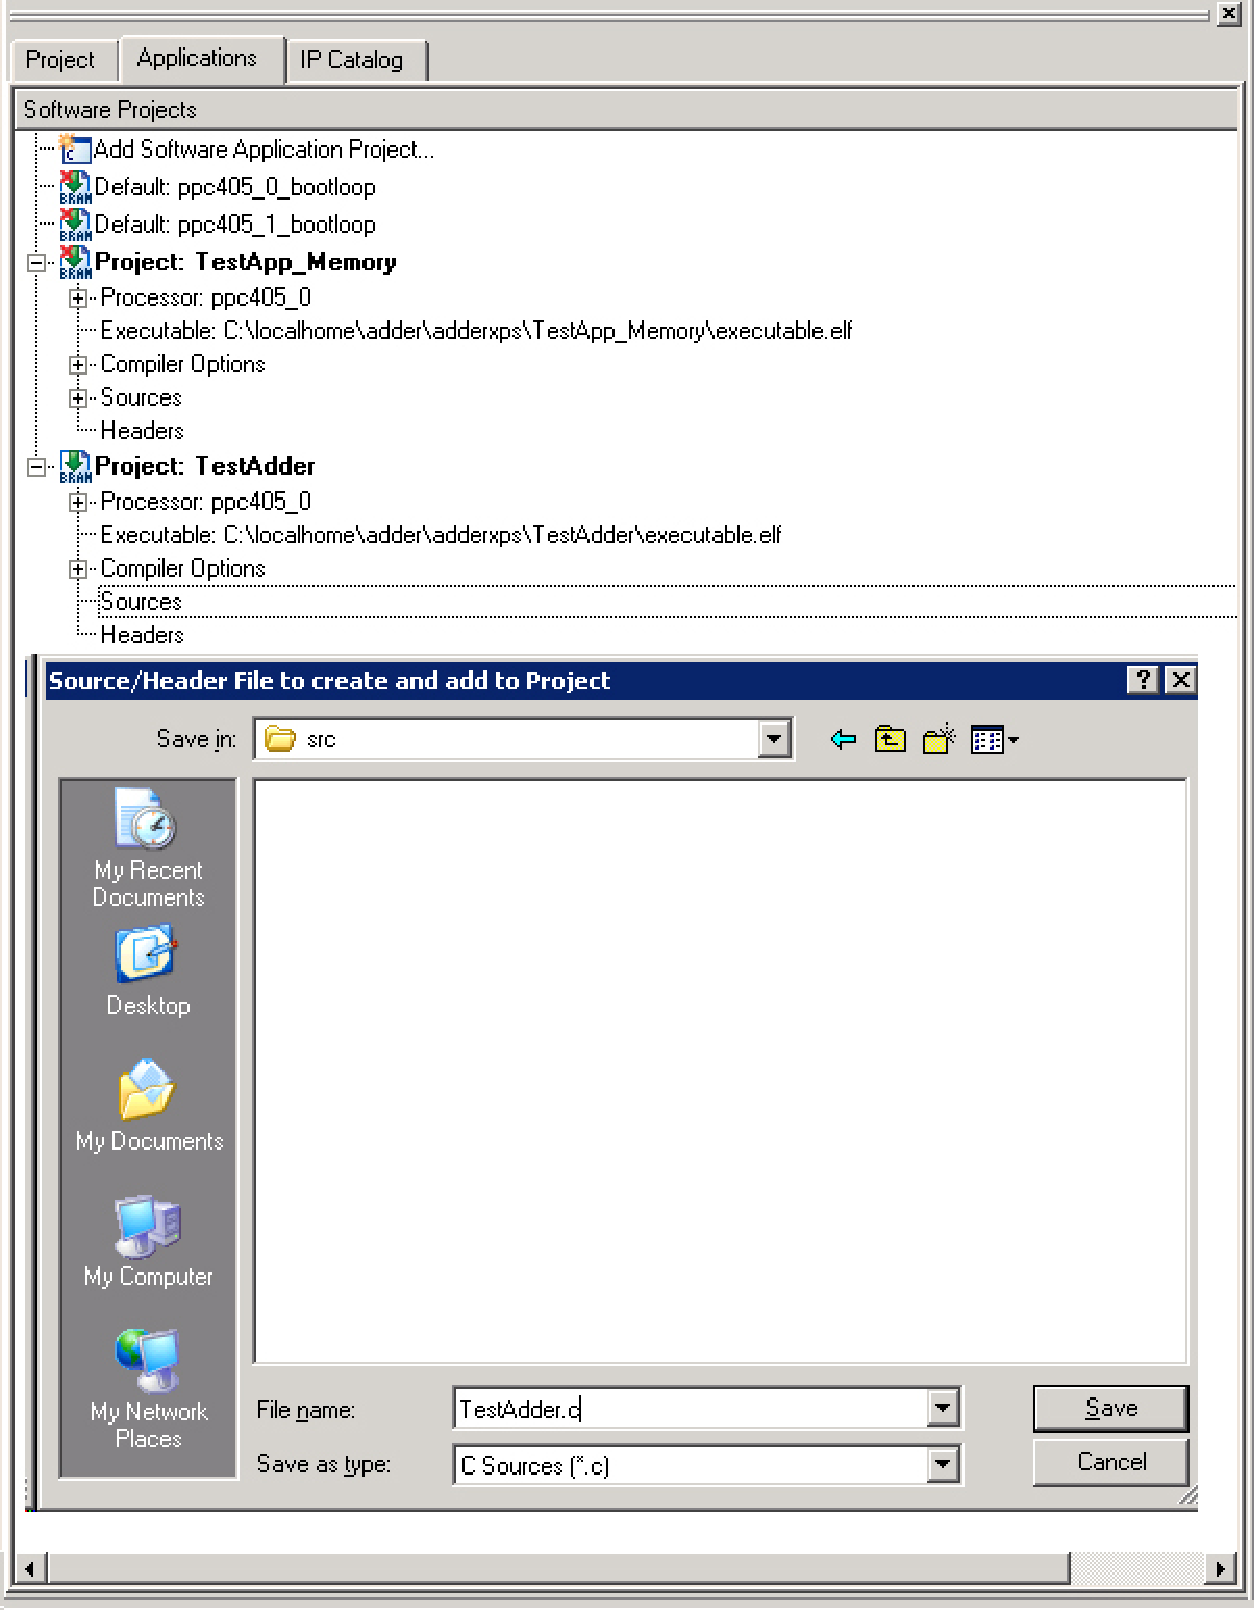
\includegraphics[width=0.40\textwidth]{ORIGdemo/21.pdf}
					\label{fig:21}
				\end{figure}
				
			\item Under Project: TestAdder, expand Sources. Double-click on the new C file that you have recently created in the previous step. Now there will be a TestAdder tab.
			\newpage
			
			\item Within the text file, type:
				\begin{figure}[htbp]
					\centering
					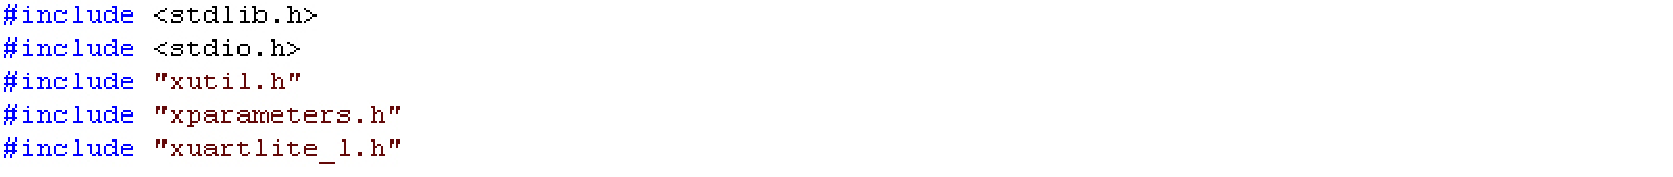
\includegraphics[width=0.90\textwidth]{ORIGdemo/code1.pdf}
					\label{fig:code1}
				\end{figure}
						
			\item Go to the directory where you created and converted the System Generator model. Double click on adder\_gatewayLog.h. This is a file that is generated when you converted the System Generator. This contains all the definitions for the register spaces within the address field. Copy all of the text to your TestAdder.c . Make sure that the copied text is below the library declarations. Here is a sample of what the code should look like now:
				\begin{figure}[htbp]
					\centering
					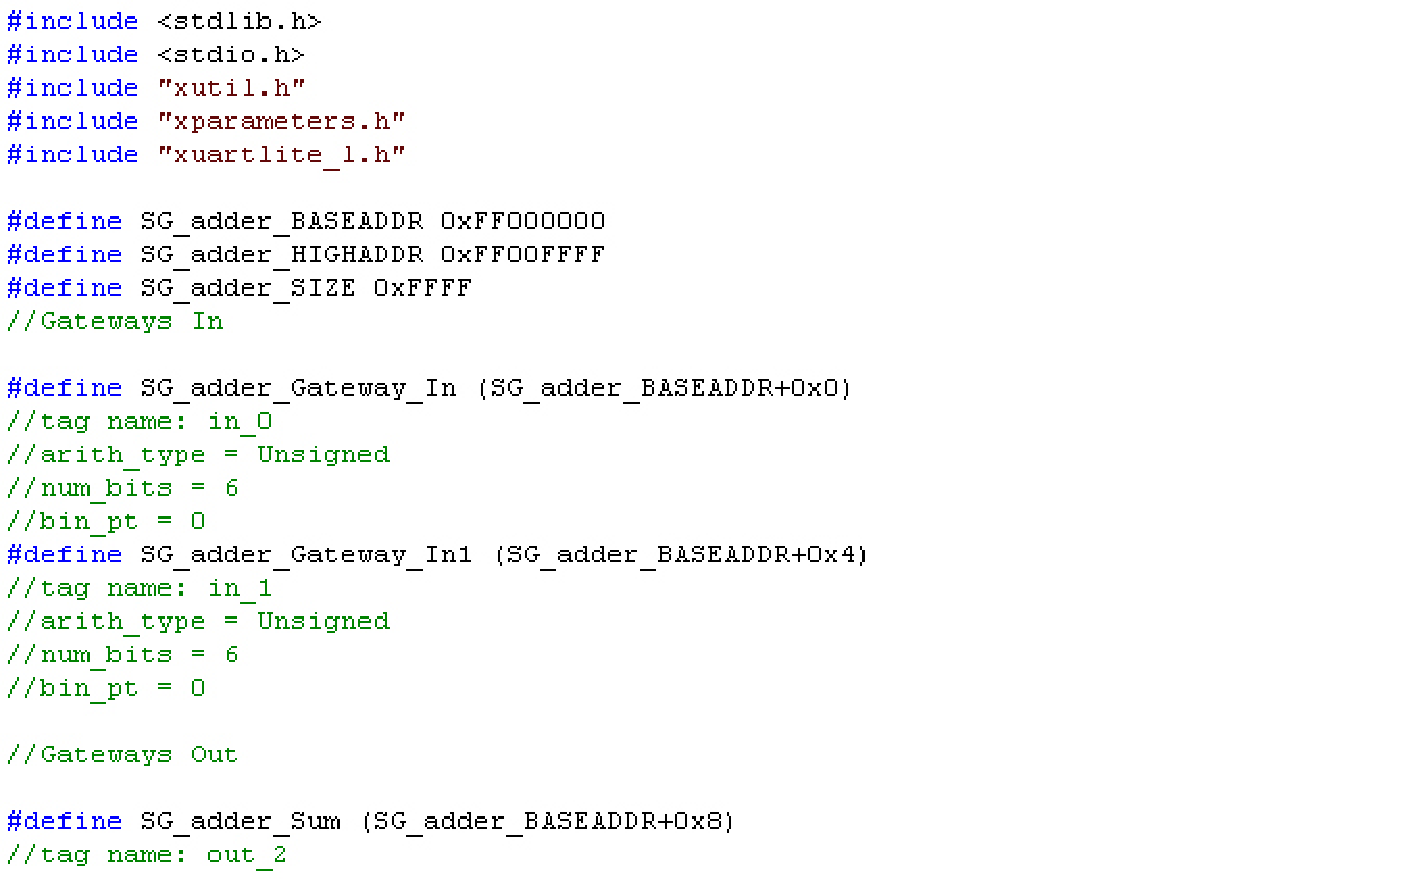
\includegraphics[width=0.90\textwidth]{ORIGdemo/code2.pdf}
					\label{fig:code2}
				\end{figure}
			
			\item Below your address definitions, type the following:
				\begin{figure}[htbp]
					\centering
					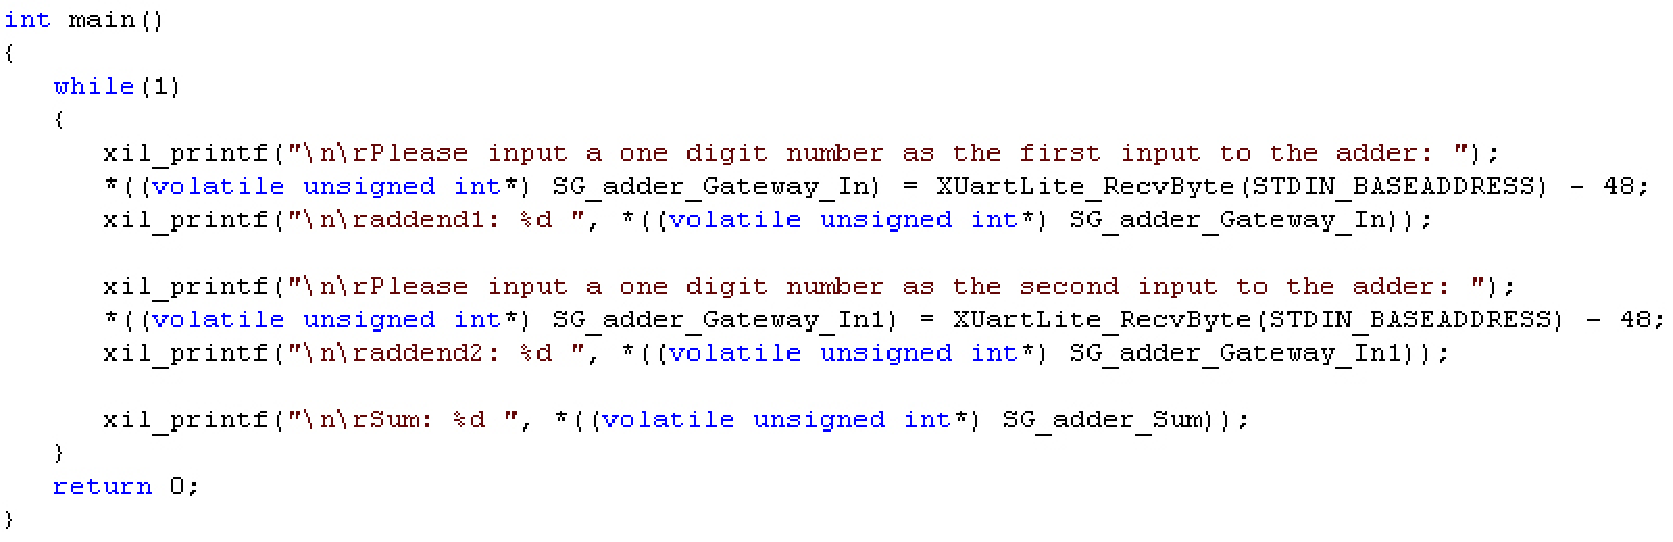
\includegraphics[width=0.90\textwidth]{ORIGdemo/code3.pdf}
					\label{fig:code3}
				\end{figure}
				\newpage

			\item This is what your code should look like in the end:
				\begin{figure}[htbp]
					\centering
					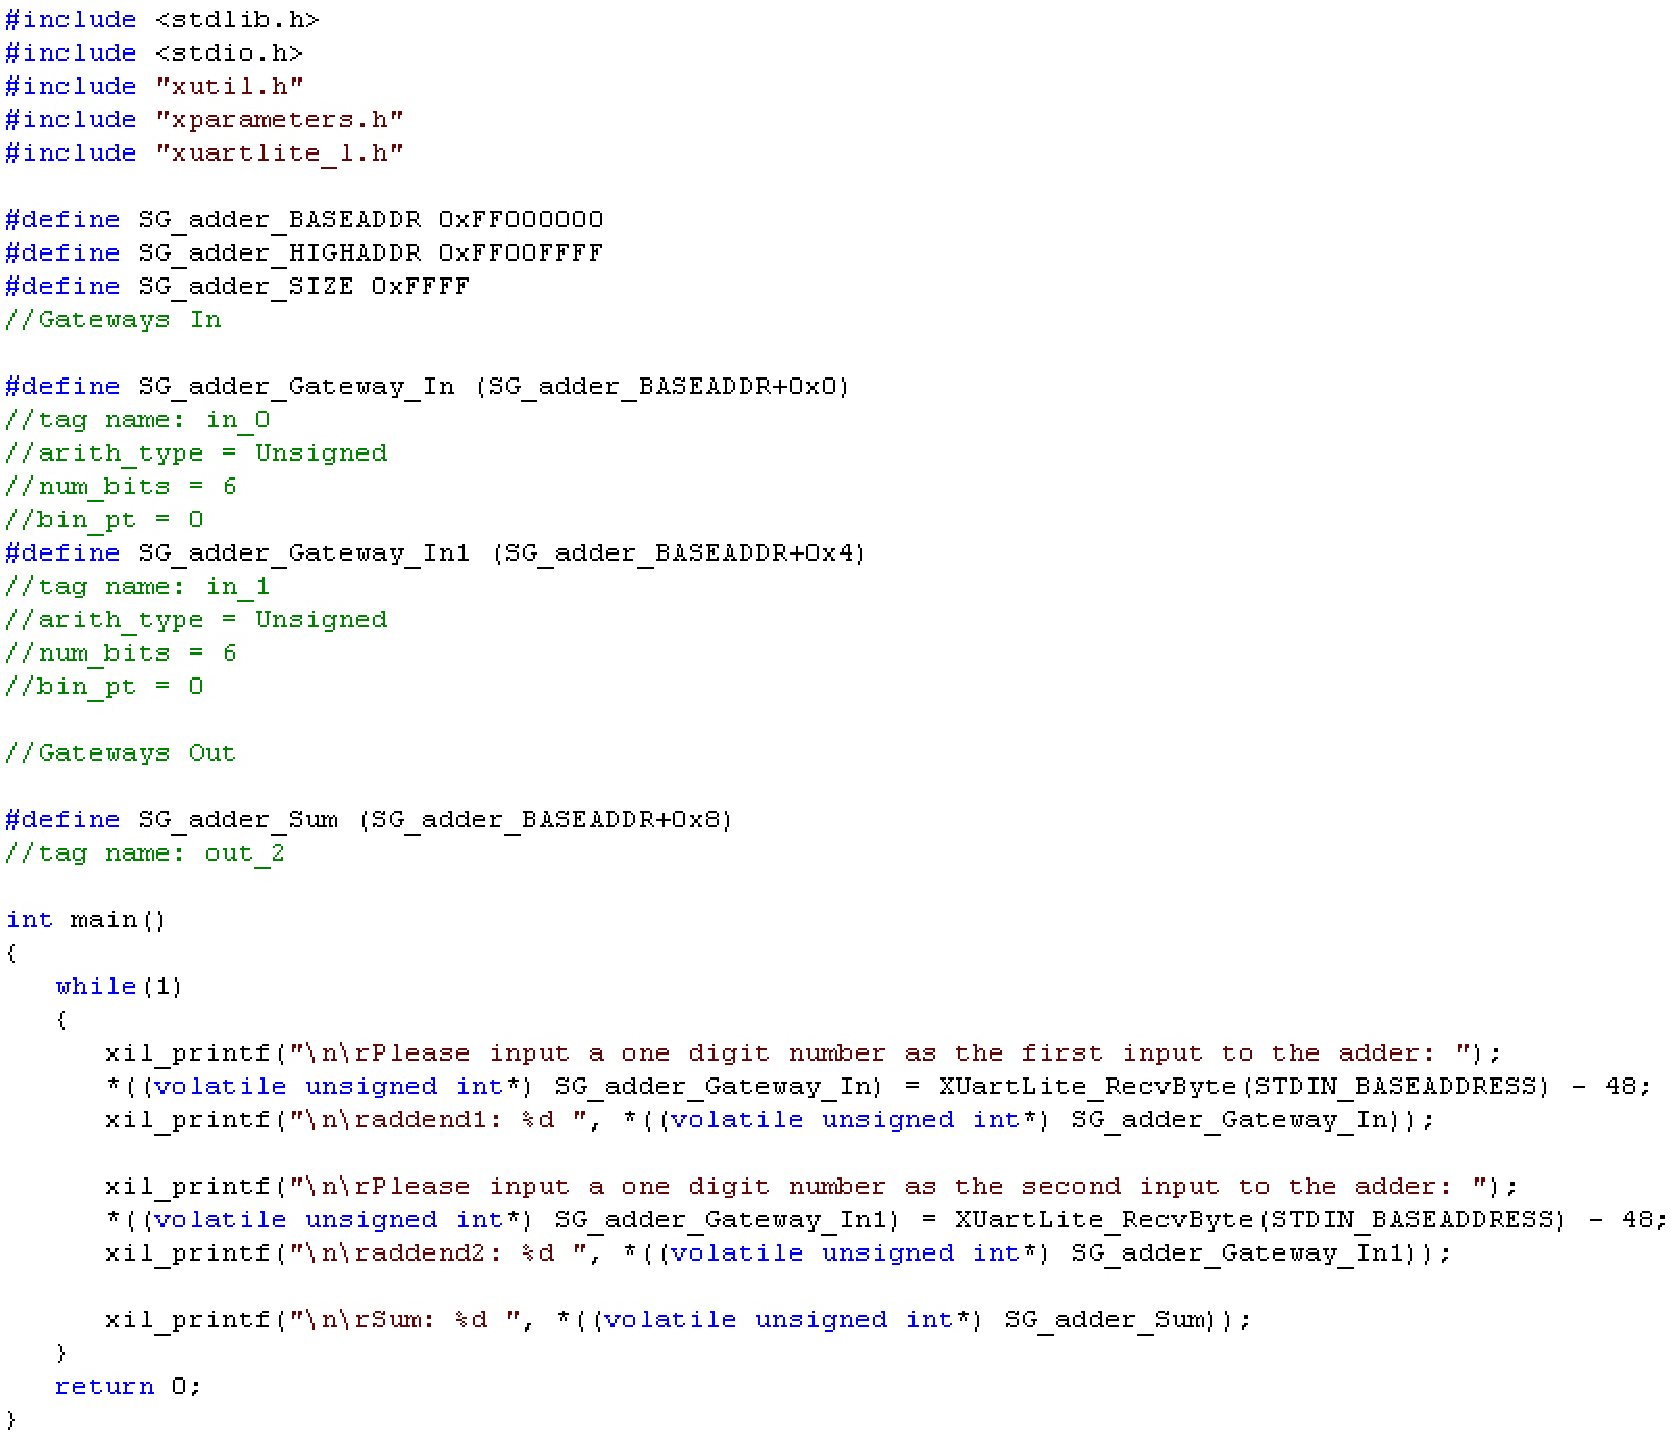
\includegraphics[width=0.90\textwidth]{ORIGdemo/code4.pdf}
					\label{fig:code4}
				\end{figure}
				
			\item On the XPS menu, go to: File $\rightarrow$ Save to save the c file.
			
			\item On the XPS menu, go to: Hardware $\rightarrow$ Generate Bitstream.
			
			\item Click on BRAM INIT on the XPS toolbar (or on the XPS menu, go to: Device Configuration $\rightarrow$ Update Bitstream).
			
		\end{enumerate}
	\subsection{Connecting the WARP Board}
		Connect the WARP board to the serial port of the computer. Turn on the power. For more information in regards to connecting the WARP board to the computer, please read the section ''Connecting and Powering the WARP FGPA Board'' within the WARP document ''WARP FPGA Board User I/O Reference Design.''
	
	\newpage
	\subsection{Tera Term}
		\begin{enumerate}
			\item Open Tera Term Pro. Select Serial. Set the Port to COM1. Press OK.
				\begin{figure}[htbp]
						\centering
						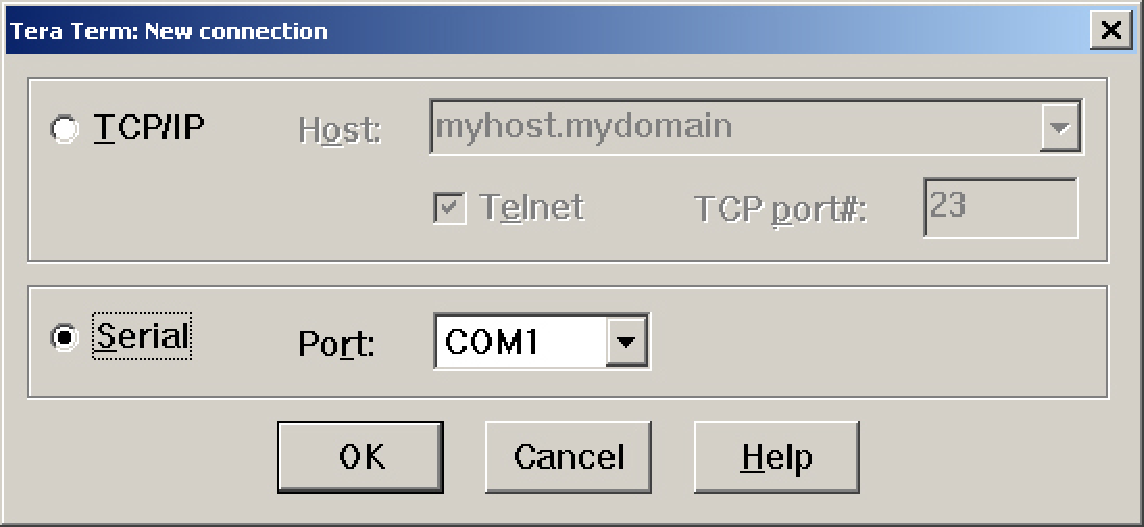
\includegraphics[width=0.40\textwidth]{ORIGdemo/23.pdf}
						\label{fig:23}
				\end{figure}
				
			\item Go to Setup $\rightarrow$ Serial Port. Verify that the baud rate is 9600. Press OK.
				\begin{figure}[htbp]
						\centering
						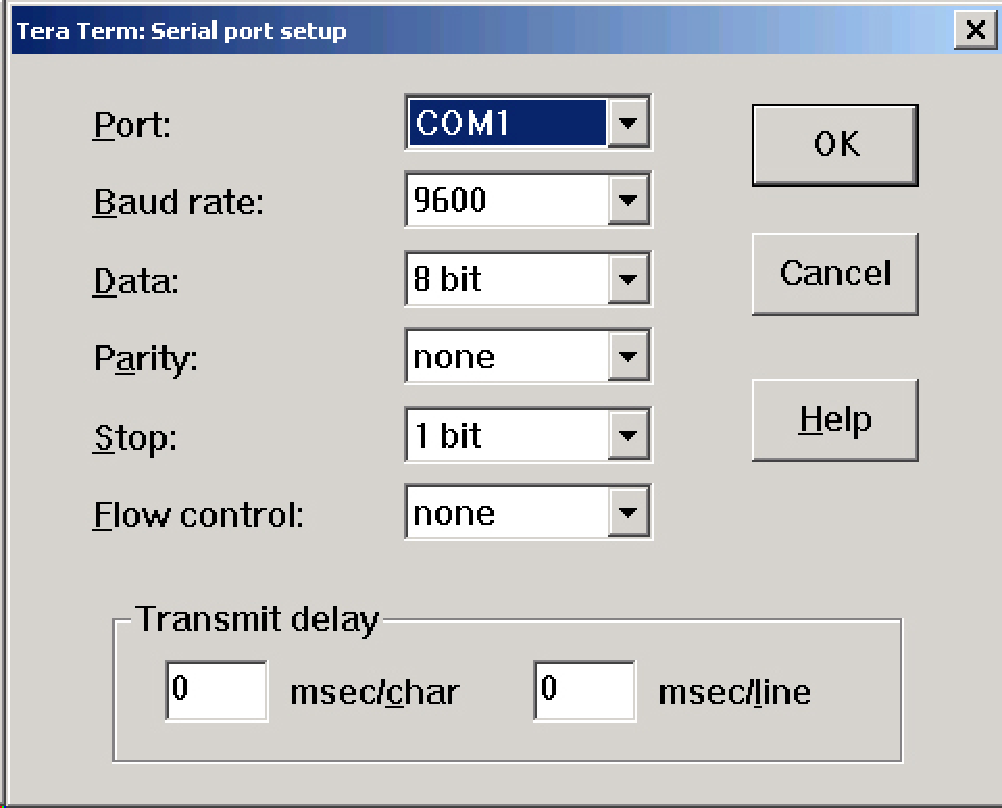
\includegraphics[width=0.40\textwidth]{ORIGdemo/24.pdf}
						\label{fig:24}
				\end{figure}
	\end{enumerate}
		
	\newpage
	\subsection{iMPACT}
		\begin{enumerate}
			\item Open Xilinx iMPACT. 
			\item Cancel the iMPACT Project dialog prompt. 
			\item Double click on Boundary Scan within the iMPACT modes tab. 
			\item Right-click on the empty project space in the Boundary Scan tab. Select Initialize Chain. 
			\item Click on Bypass for the first prompt.
			\item On the second prompt, to your directory where you saved your XPS project. Double click on the implementation folder and select download.bit . Click Open.
				\begin{figure}[htbp]
						\centering
						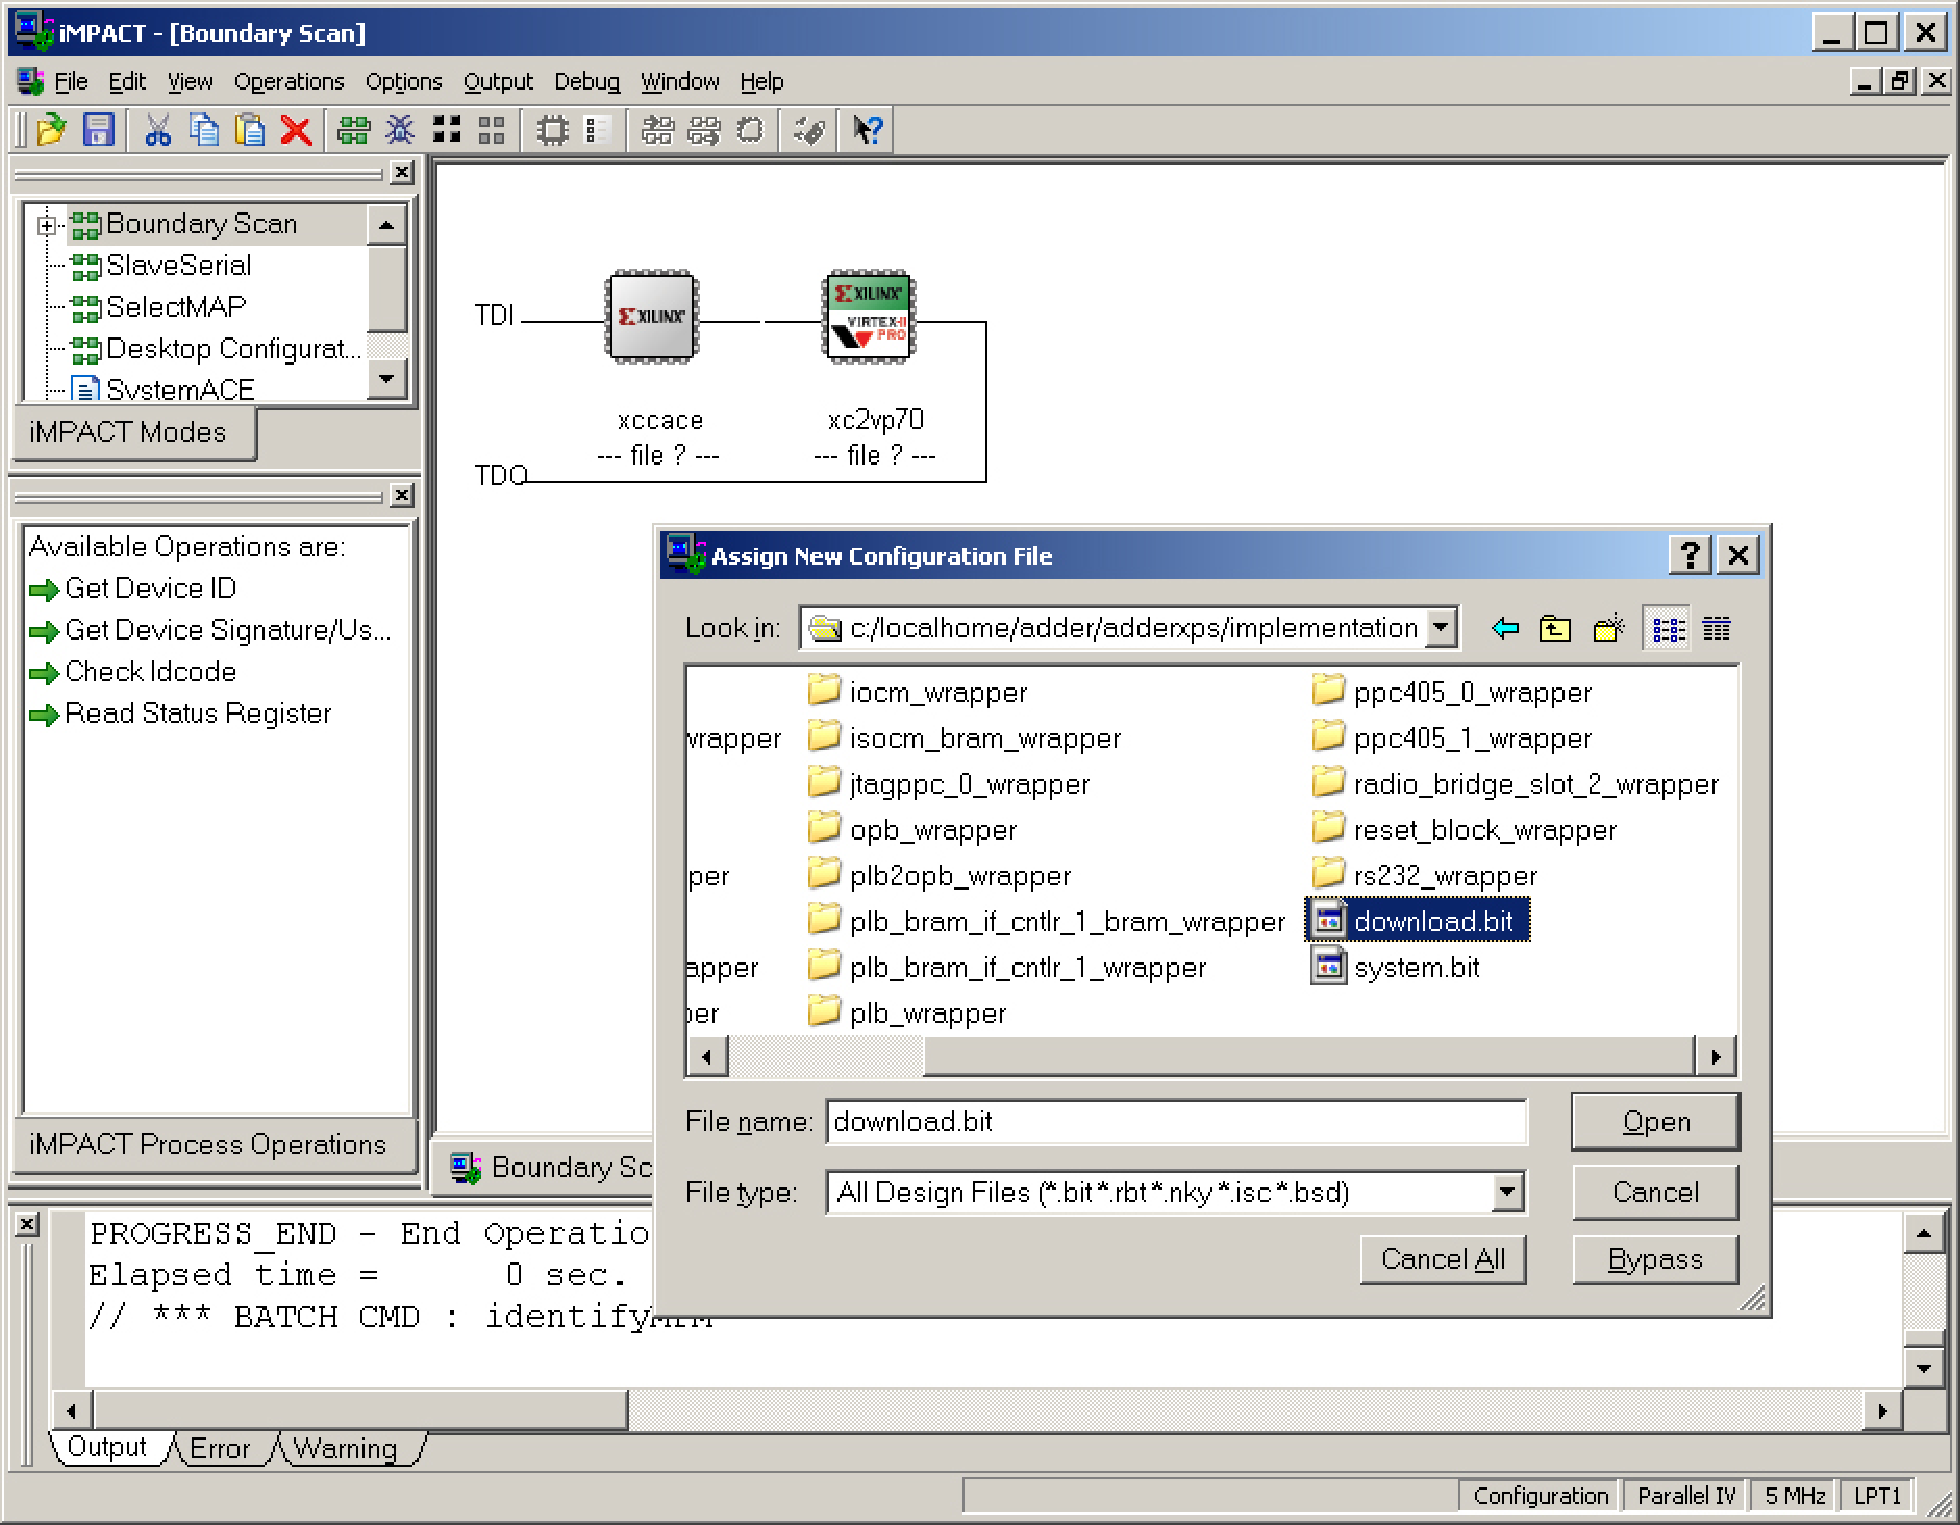
\includegraphics[width=0.40\textwidth]{ORIGdemo/25.pdf}
						\label{fig:25}
				\end{figure} 
			\item Select OK on the resulting prompt.
				\begin{figure}[htbp]
						\centering
						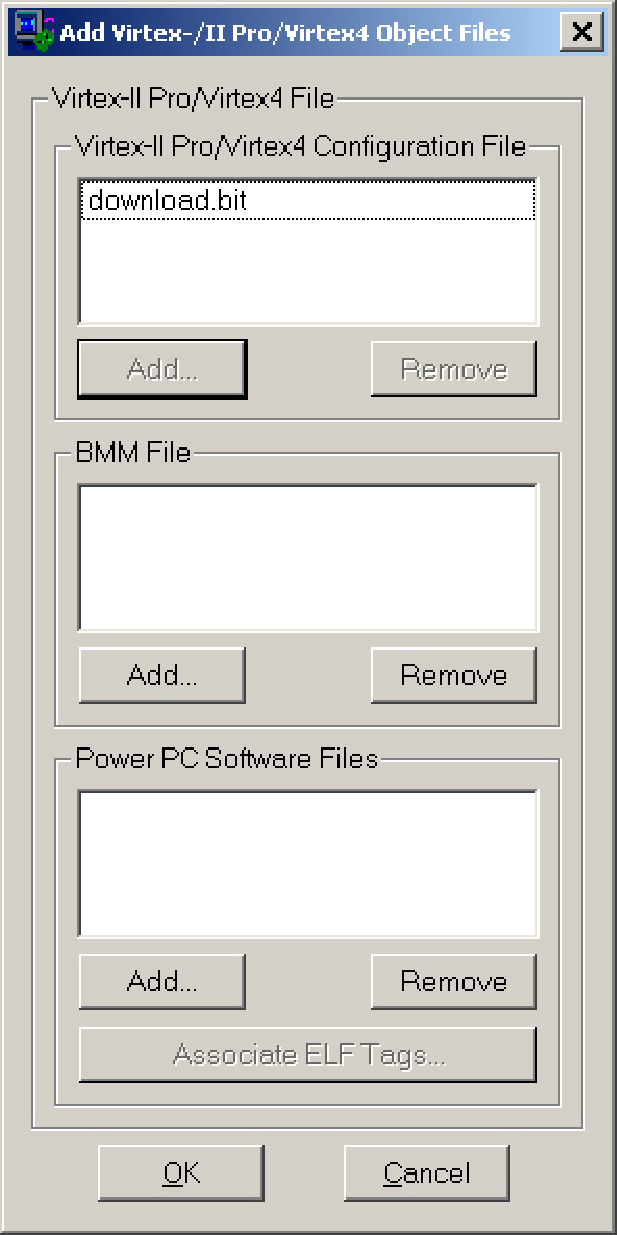
\includegraphics[width=0.30\textwidth]{ORIGdemo/26.pdf}
						\label{fig:26}
				\end{figure}
				\newpage
			\item Right-click on xc2vp70 download.bit . Select Program. 
				\begin{figure}[htbp]
						\centering
						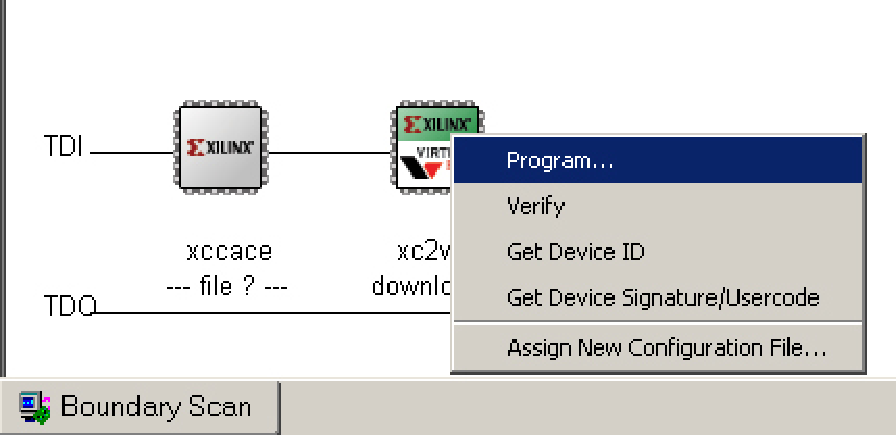
\includegraphics[width=0.40\textwidth]{ORIGdemo/27.pdf}
						\label{fig:27}
				\end{figure}
			\item Click OK on Programming Properties.
				\begin{figure}[htbp]
						\centering
						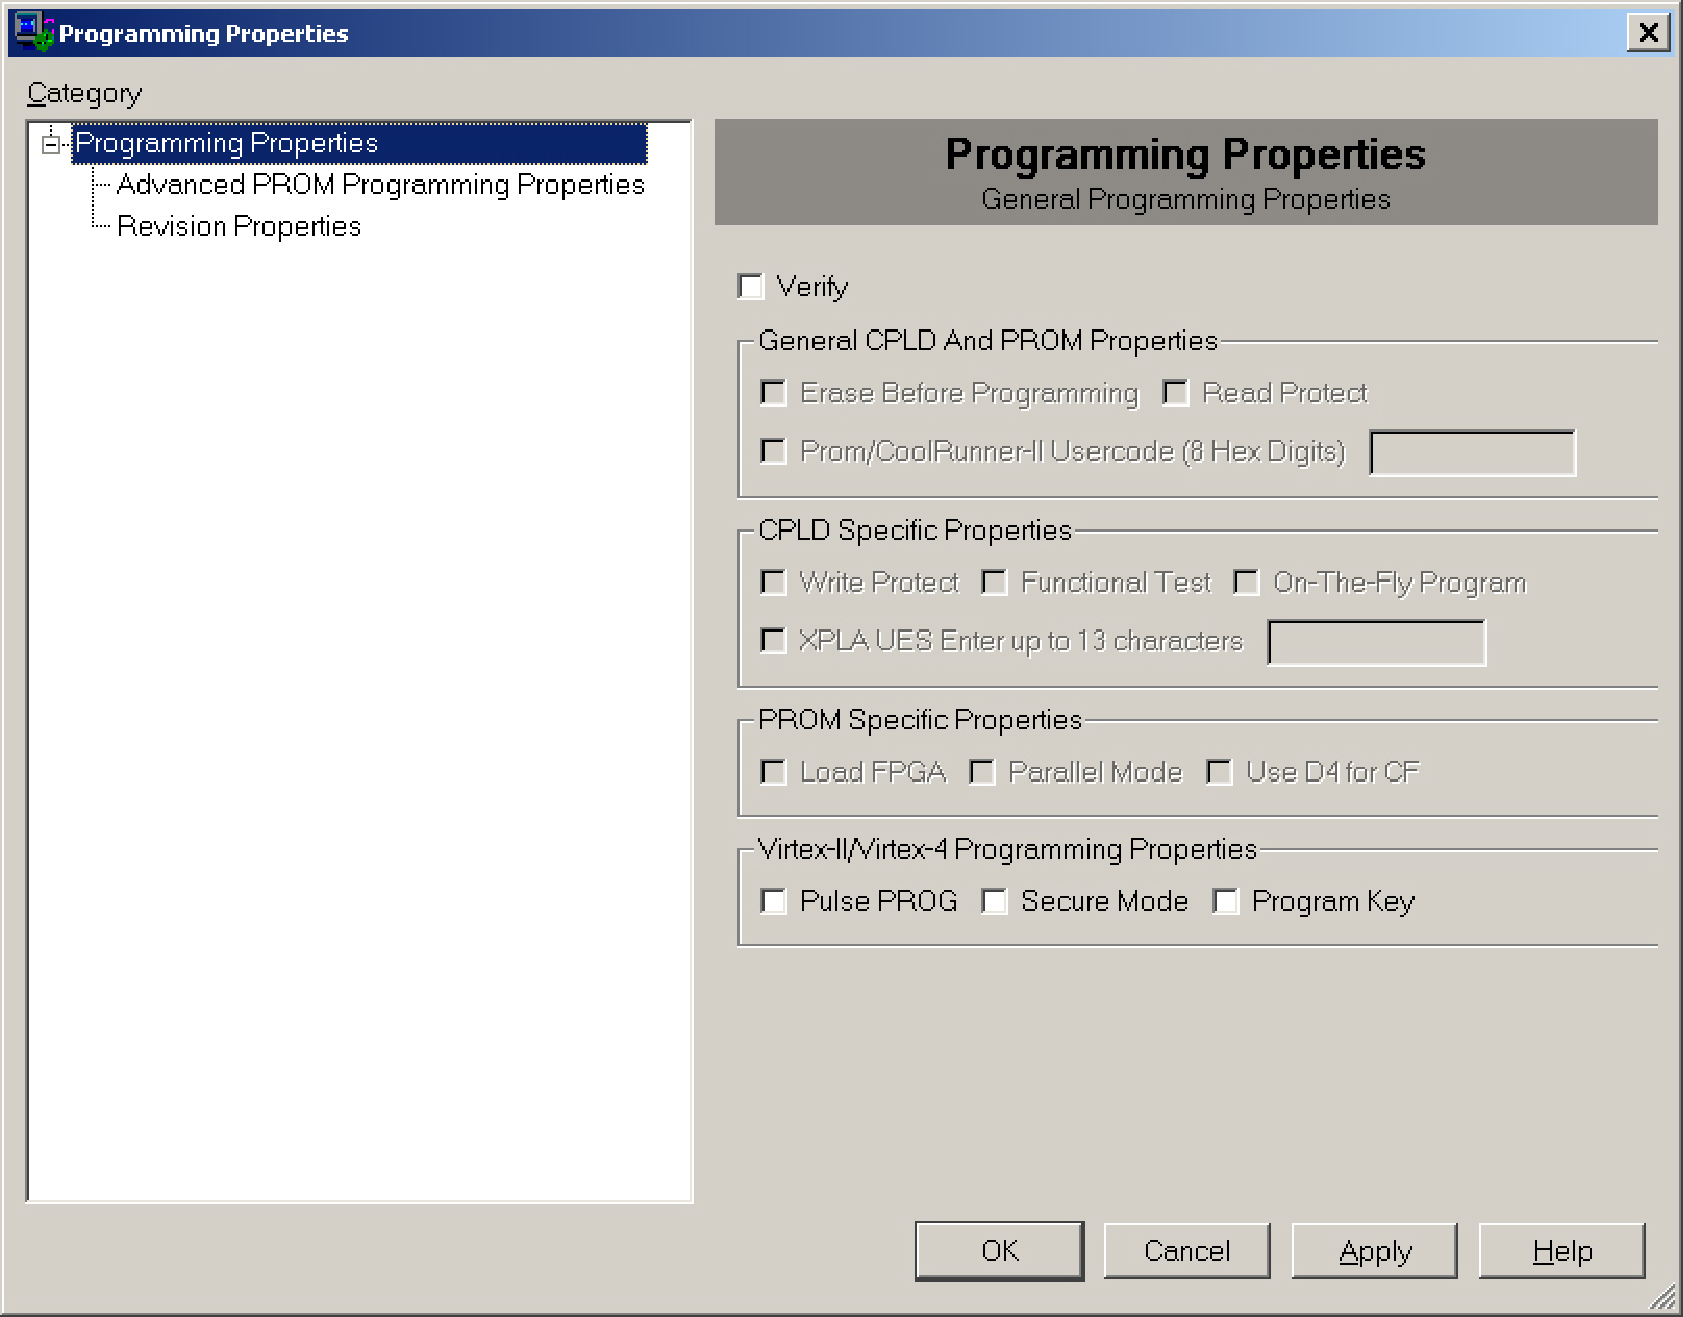
\includegraphics[width=0.40\textwidth]{ORIGdemo/28.pdf}
						\label{fig:28}
				\end{figure}
			\item After it says Program Succeeded, go back to your tera term window and try different inputs for the program.
		\end{enumerate} 





\newpage
\section{Example with Read Only Shared Memory Extension}

\subsection{Requirements}
This example assumes that you already know how to use Simulink/Xilinx System Generator, create a XPS project, add a pcore to the XPS project, edit the different properties of System Assembly within XPS, add a Software Application Project, generate the bitstream for the project, use Tera Term, and use iMPACT. If not please go to ''Example with the Original Script'' in this documentation and go through the demo.
\\
\\This example uses System Generator 8.1, XPS 8.1, and the iMPACT Tool associated with Xilinx ISE 8.1i

\subsection{Xilinx Platform Studio - Base System Builder}
Create XPS project. Use Base System Builder to build the project.

\subsection{Matlab/System Generator}
\begin{enumerate}
	\item Open Matlab and Simulink
	\item Create a new model. Save it as SMROdemo.mdl .
	\item Add the following blocks and edit their properties:
		\begin{enumerate}
			\item Xilinx Blockset/Basic Elements/System Generator
			\item Simulink/Sources/Constant
				\begin{enumerate}
					\item Name: Constant
					\item Constant value: 5
					\item Sample time: 1
				\end{enumerate}
			\item Simulink/Sources/Counter Free-Running
				\begin{enumerate}
					\item Name: Counter Free-Running
					\item Number of Bits: 14
					\item Sample time: 1
				\end{enumerate}
			\item Xilinx Blockset/Basic Elements/Gateway In
				\begin{enumerate}
					\item Name: Gateway In1
					\item Output type: Unsigned
					\item Number of bits: 14
					\item Binary point: 0
				\end{enumerate}
			\item Xilinx Blockset/Basic Elements/Gateway In
				\begin{enumerate}
					\item Name: SMROAddr\_gw
					\item Output type: Unsigned
					\item Number of bits: 14
					\item Binary point: 0
				\end{enumerate}
			\item Xilinx Blockset/Basic Elements/Constant
				\begin{enumerate}
					\item Name: Constant1
					\item Type: Unsigned
					\item Constant value: 0
					\item Number of bits: 32
					\item BInary point: 0
				\end{enumerate}
			\item Xilinx Blockset/Basic Elements/Constant
				\begin{enumerate}
					\item Name: Constant 2
					\item Type: Boolean
					\item Constant value: 0
				\end{enumerate}
			\item Xilinx Blockset/Basic Elements/Constant
				\begin{enumerate}
					\item Name: SMRODataI\_const
					\item Type: Unsigned
					\item Constant value: 0
					\item Number of btis: 32
					\item Binary: 0
				\end{enumerate}
			\item Xilinx Blockset/Basic Elements/Constant
				\begin{enumerate}
					\item Name: SMROWE\_const
					\item Type: Boolean
					\item Constant value: 0
				\end{enumerate}
			\item Xilinx Blockset/Memory/Dual Port RAM
				\begin{enumerate}
					\item Depth: \verb|2^14|
					\item Initial value vector: 1:16384
					\item Latency: 1 
				\end{enumerate}
			\item Xilinx Blockset/Basic Elements/Gateway Out
				\begin{enumerate}
					\item Name: Gateway Out1
				\end{enumerate}
			\item Xilinx Blockset/Basic Elements/Gateway Out
				\begin{enumerate}
					\item Name: SMRODataO\_GW
				\end{enumerate}
			\item Simulink/Commonly Used Blocks/Scope
				\begin{enumerate}
					\item Name: Scope
					\item Number of axes: 2
						\\Double click on Scope. Click on Scope parameters (the second button on the Scope toolbar).
Set Number of aces to 2. Click OK. Exit the scope. Now the Scope should have 2 inputs.
				\end{enumerate}
		\end{enumerate}
	\newpage
	\item Connect Constant to Gateway In1. Connect Gateway In1 to the addra port of SMRO\_dpram. Connect Constant1 to the dina port of SMRO\_dpram. Connect Constant2 to the wea port of SMRO\_dpram. Connect Counter Free-Running to SMROAddr\_gw. Connect SMROAddr\_gw to addrb. Connect SMRODataI\_const to dinb. Connect SMROWE\_const to web. Connect SMRO\_dpram outport A to Gateway Out1. Connect Gateway Out1 outport to the first inport of Scope. Connect SMRO\_dpram outport B to SMRODataO\_GW. Connect SMRODataO\_GW to second inport of Scope.
		\begin{figure}[htbp]
			\centering
			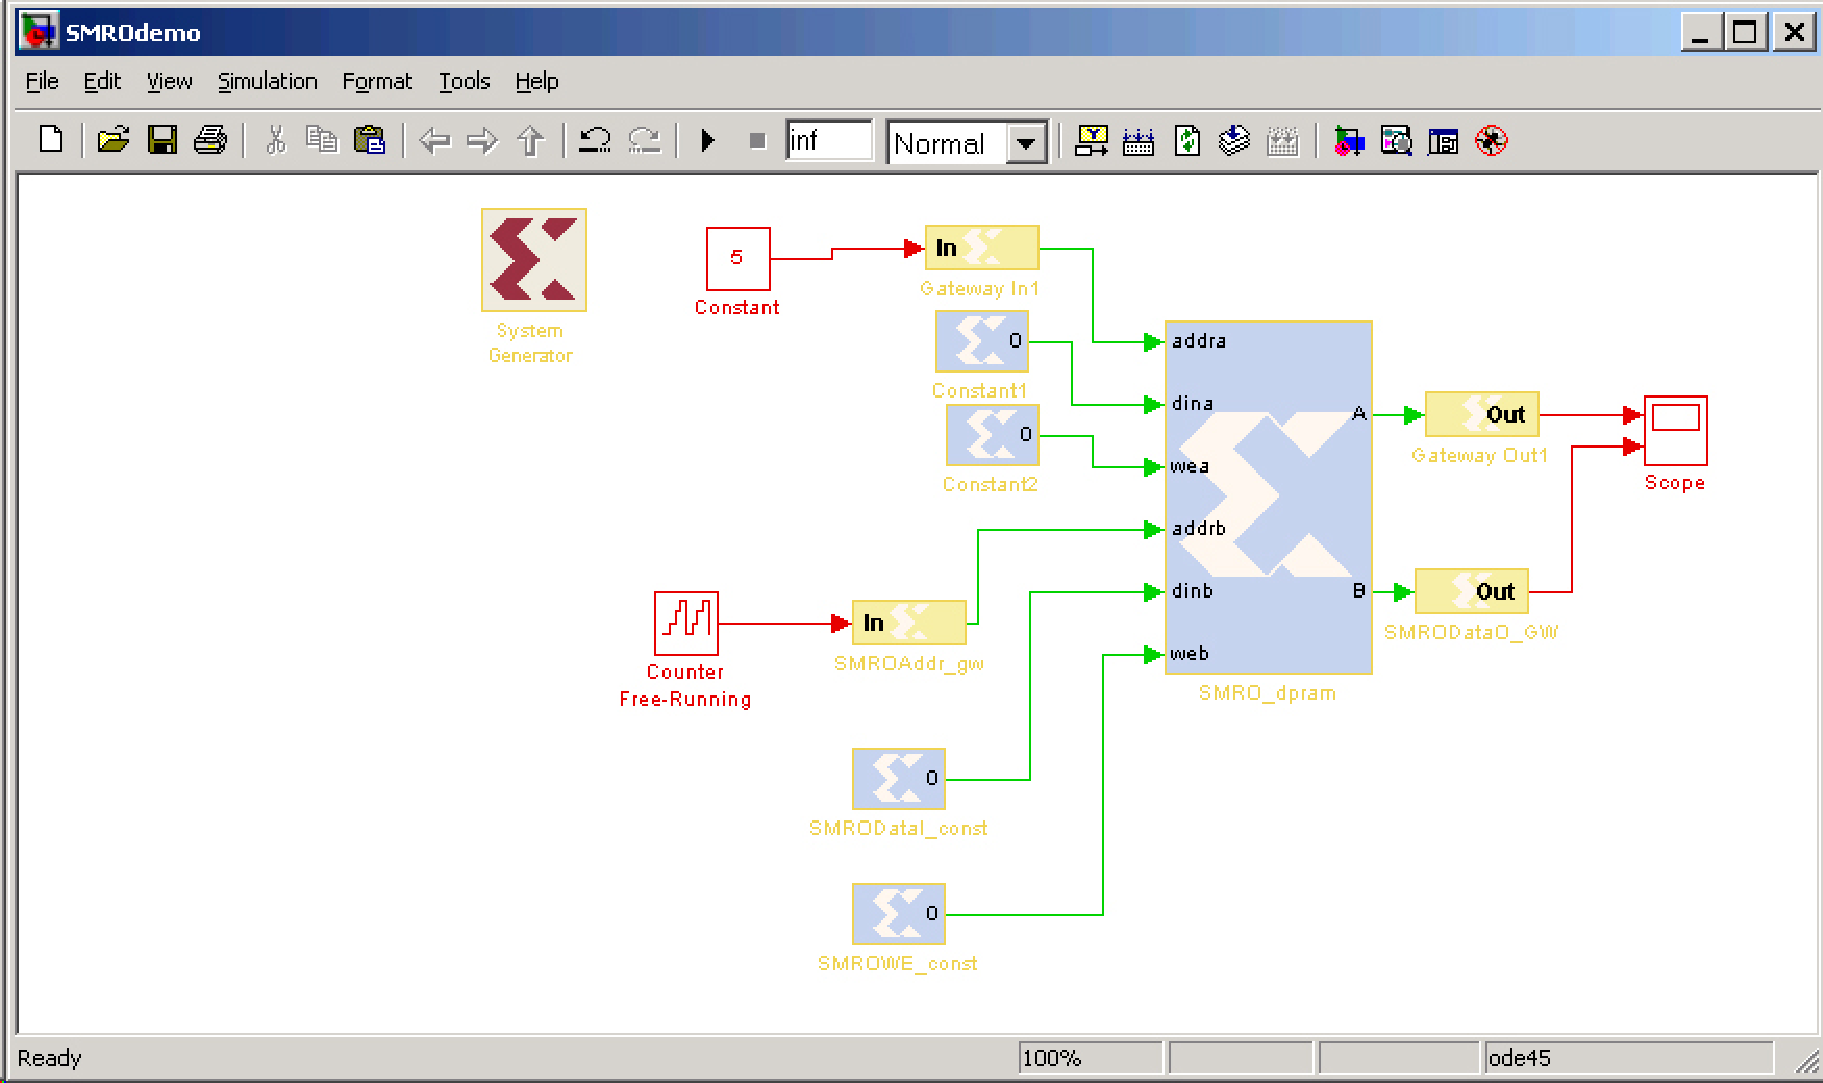
\includegraphics[width=0.70\textwidth]{SMROdemo/UnconvertedModel.pdf}
			\caption{Unconverted Model}
			\label{fig:UnconvertedModelSMRO}
		\end{figure}
	\item Run the script:
	  \\sysgen2opb('SMROdemo', hex2dec('FF000000'), 'sm')
	  	\begin{figure}[htbp]
				\centering
				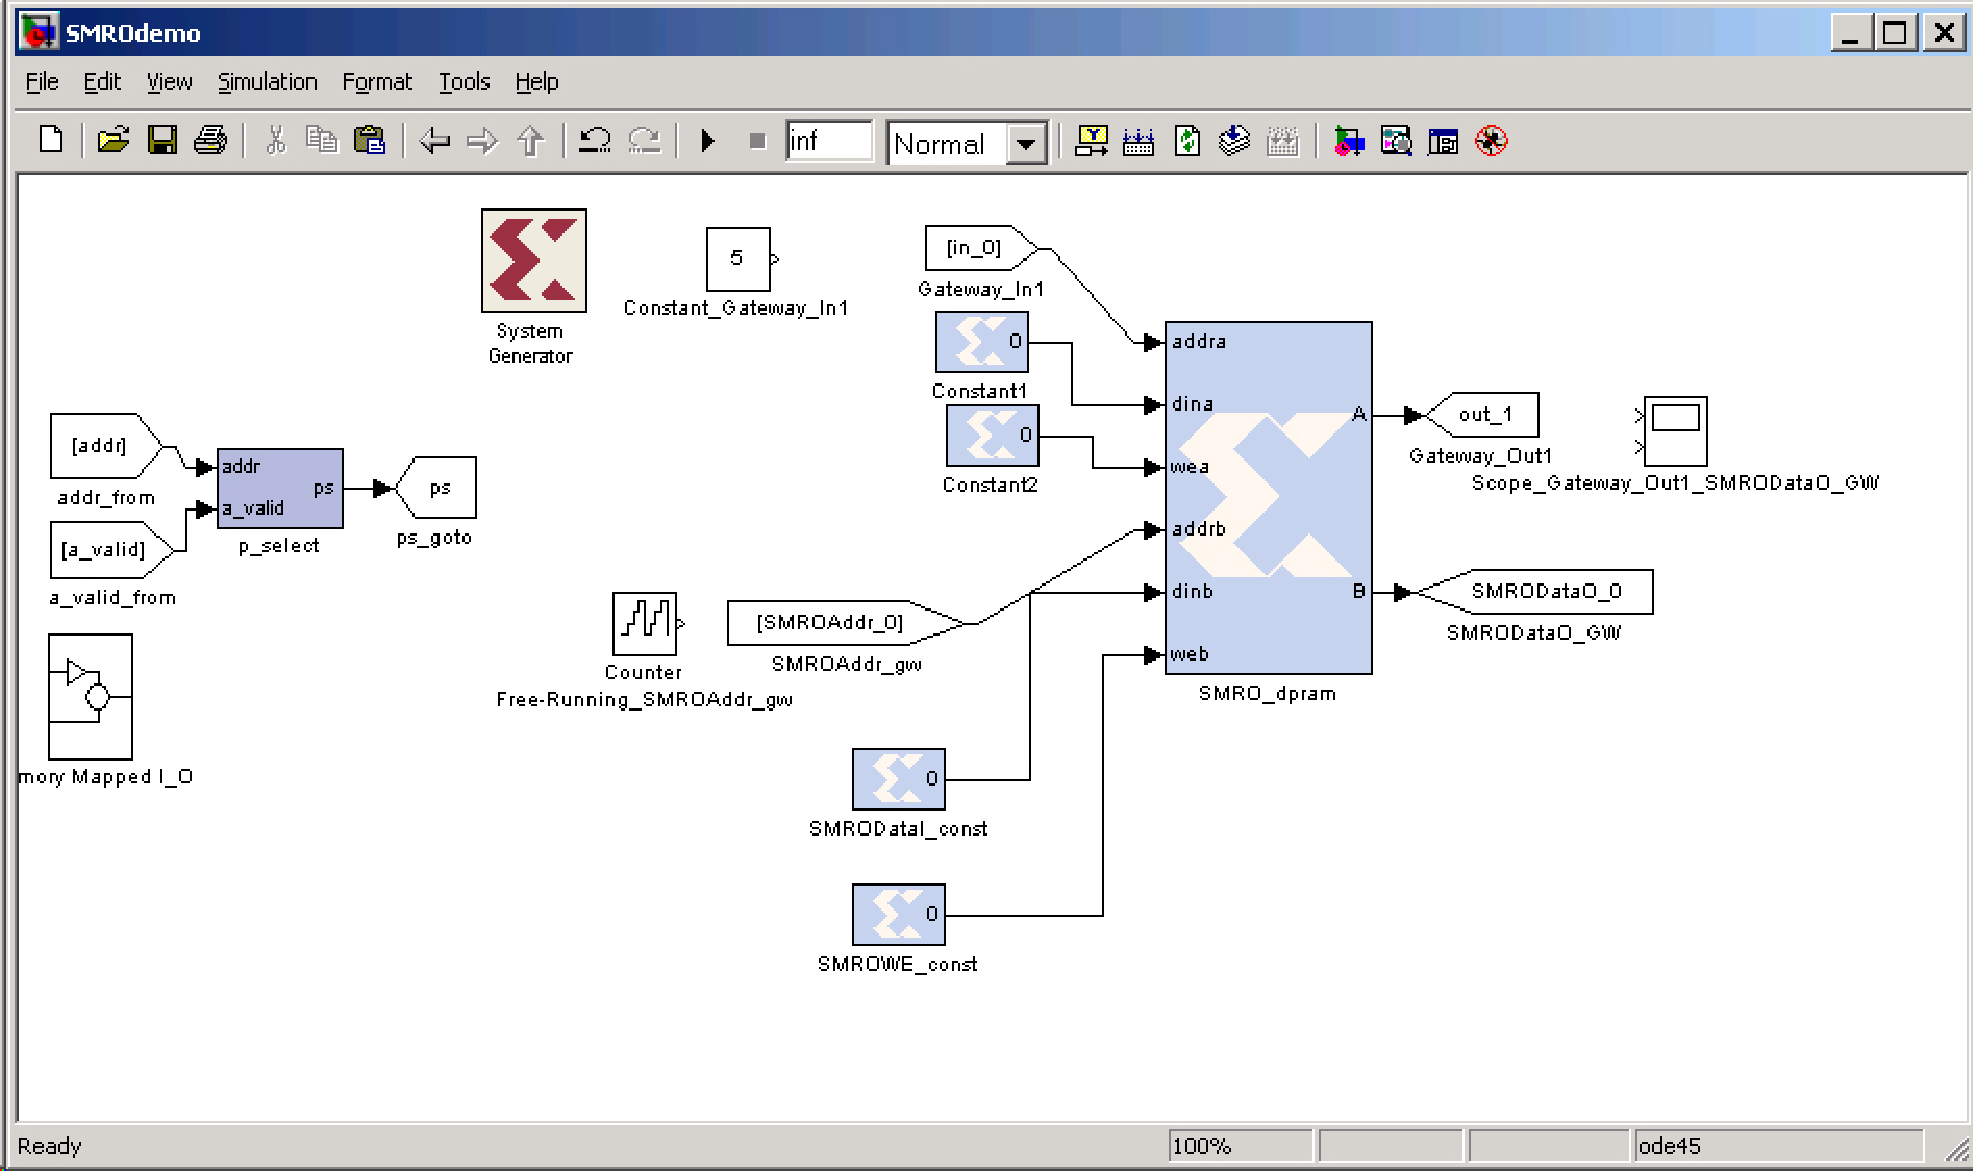
\includegraphics[width=0.70\textwidth]{SMROdemo/ConvertedModel.pdf}
				\caption{Converted Model}
				\label{fig:ConvertedModelSMRO}
			\end{figure}
	\item Use System Generator to generate the HDL.
\end{enumerate}

\subsection{Xilinx Platform Studio}
\begin{enumerate}
	\item After creating the project, add the generated pcore to the XPS Project.
	\item Edit the different properties of System Assembly within XPS.
	\item Add a Software Application Project. Name the project TestSMROdemo. Create a new C Source file. Name the file ''TestSMROdemo.c''
	\item After including the necessary libraries and copying the generated .h file \\(SMROdemo\_gatewaySMLog.h), add in the following code:
		\begin{figure}[htbp]
			\centering
			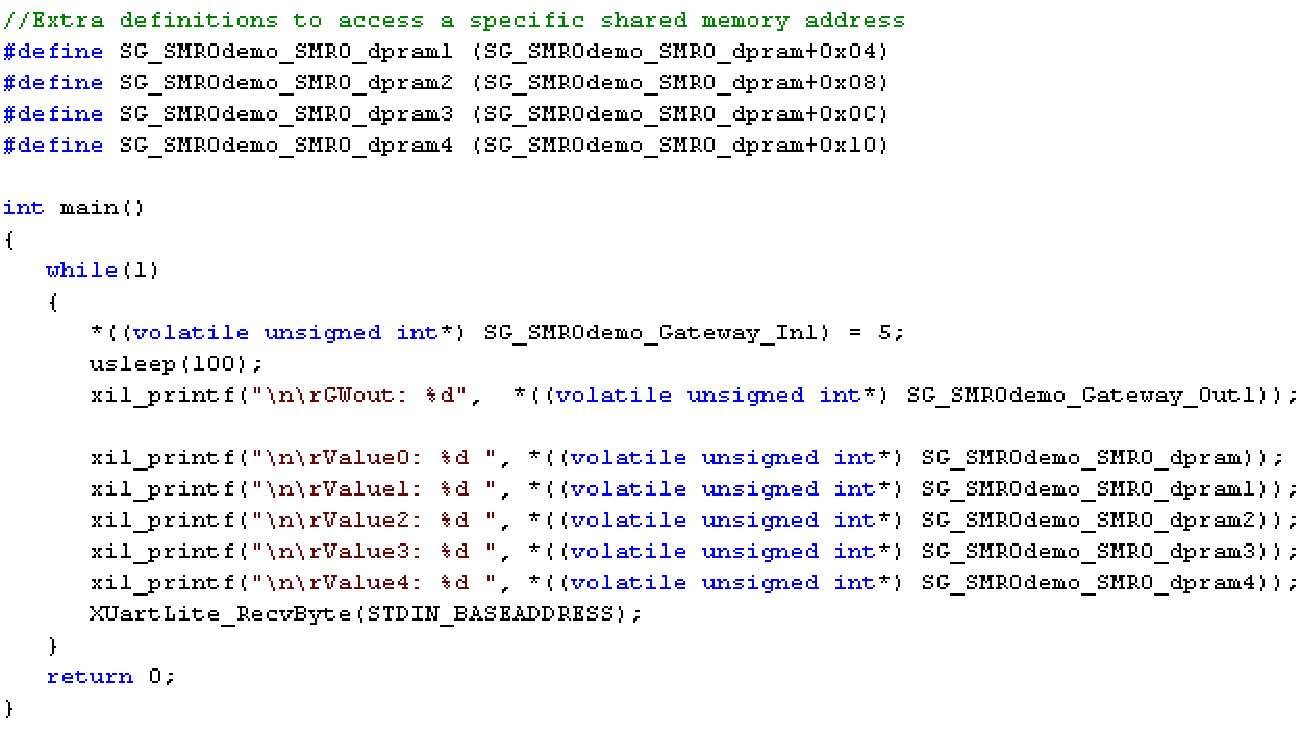
\includegraphics[width=0.90\textwidth]{SMROdemo/code1.pdf}
			\label{fig:codeSMRO1}
		\end{figure}
	\newpage
	\item This is what the code should look like:
		\begin{figure}[htbp]
			\centering
			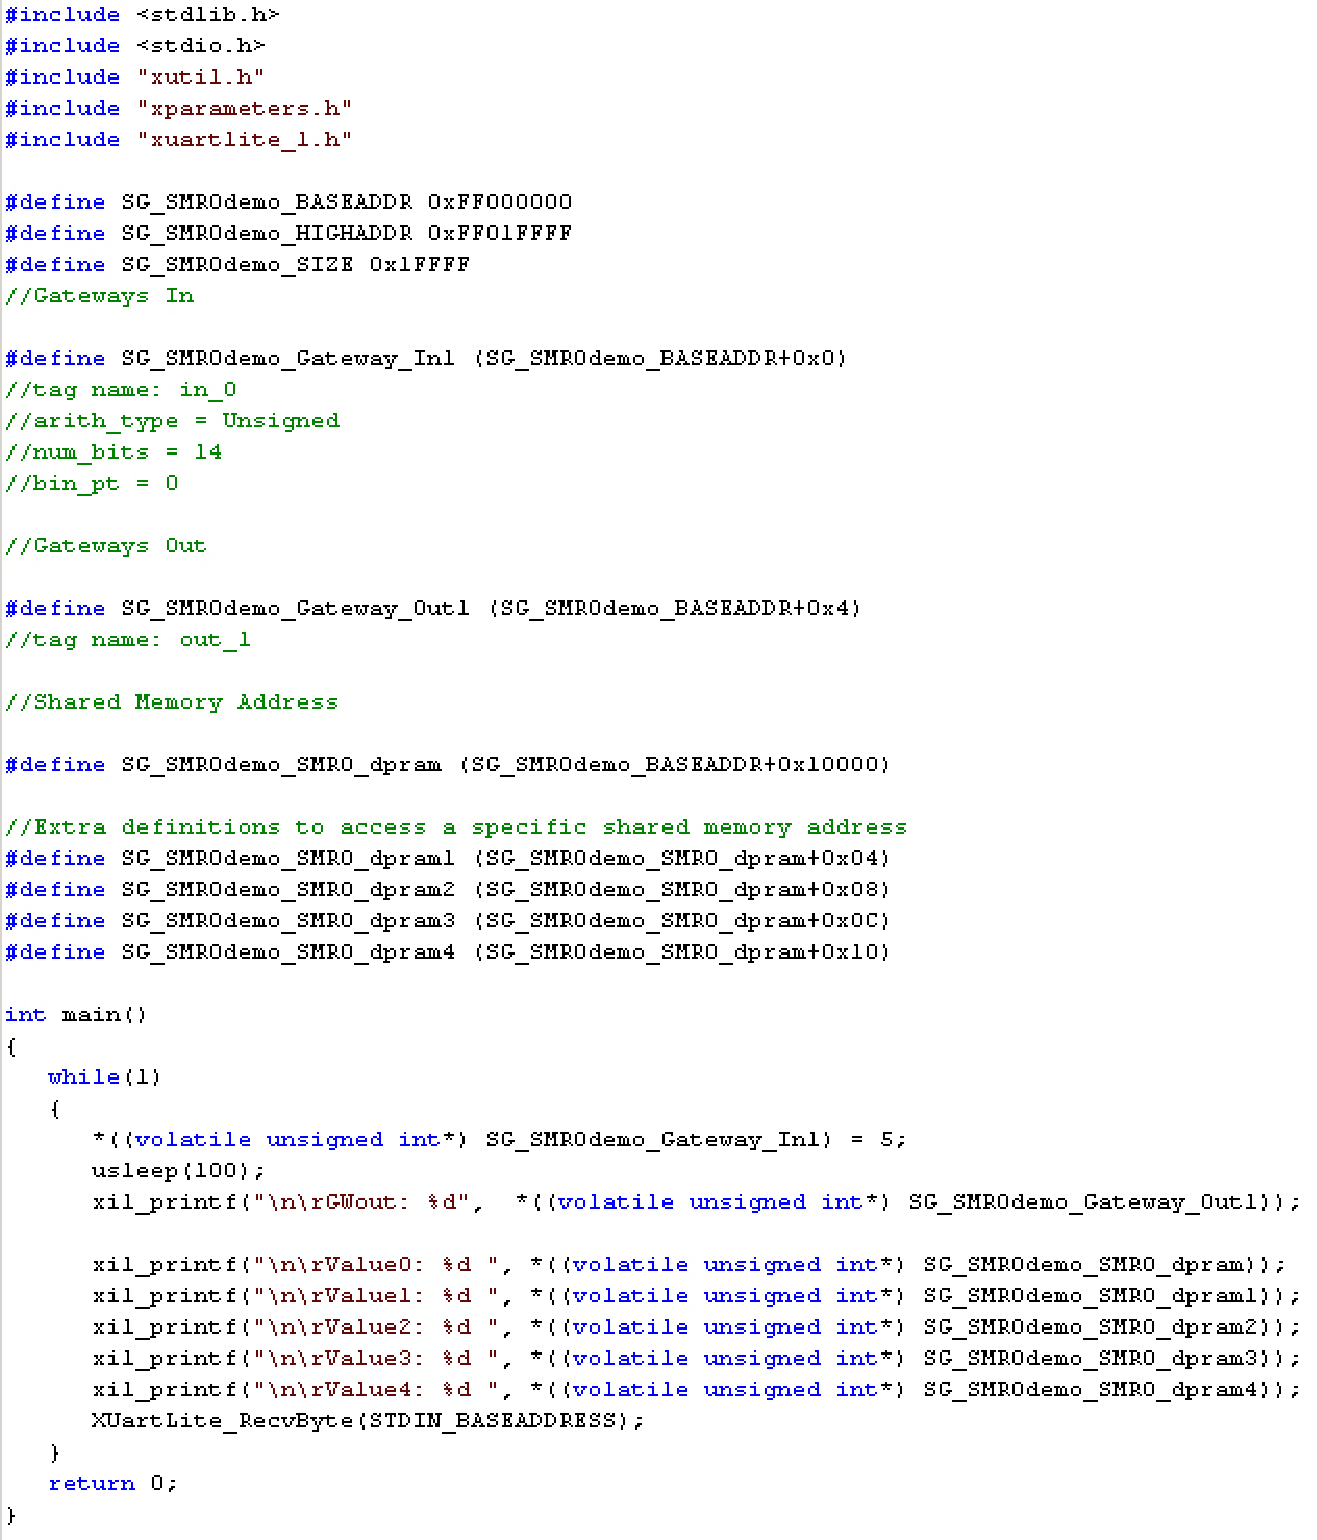
\includegraphics[width=0.90\textwidth]{SMROdemo/code2.pdf}
			\label{fig:codeSMRO2}
		\end{figure}
	\item Save the file. Generate the bitstream. Update the bitstream. Put the bitstream onto the board and view the output.
		
\end{enumerate}

\newpage





\section{Example with Write Only Shared Memory Extension}
\subsection{Requirements}
This example assumes that you already know how to use Simulink/Xilinx System Generator, create a XPS project, add a pcore to the XPS project, edit the different properties of System Assembly within XPS, add a Software Application Project, generate the bitstream for the project, use Tera Term, and use iMPACT. If not please go to ''Example with the Original Script'' in this documentation and go through the demo.
\\
\\This example uses System Generator 8.1, XPS 8.1, and the iMPACT Tool associated with Xilinx ISE 8.1i

\subsection{Xilinx Platform Studio - Base System Builder}
Create XPS project. Use Base System Builder to build the project.

\subsection{Matlab/System Generator}
\begin{enumerate}
	\item Open Matlab and Simulink
	\item Create a new model. Save it as SMWOdemo.mdl .
	\item Add the following blocks and edit their properties:
	\begin{enumerate}
		\item Xilinx Blockset/Basic Elements/System Generator
		\item Xilinx Blockset/Basic Elements/Gateway In
			\begin{enumerate}
				\item Name: Gateway In
				\item Output type: Unsigned
				\item Number of bits: 14
				\item Binary point: 0
				\item Sample period: 1
			\end{enumerate}
		\item Xilinx Blockset/Basic Elements/Gateway In
			\begin{enumerate}
				\item Name: SMWOAddr\_gwin
				\item Output type: Unsigned
				\item Number of bits: 14
				\item Binary point: 0
				\item Sample period: 1 
			\end{enumerate}
		\item Xilinx Blockset/Basic Elements/Gateway In
			\begin{enumerate}
				\item Name: SMWODataI\_gwin
				\item Output type: Unsigned
				\item Number of bits: 32
				\item Binary point: 0
				\item Sample period: 1
			\end{enumerate}
		\item Xilinx Blockset/Basic Elements/Gateway In
			\begin{enumerate}
				\item Name: SMWOWE\_gwin
				\item Output type: Boolean
				\item Sample period: 1
			\end{enumerate}
		\item Xilinx Blockset/Basic Elements/Constant
			\begin{enumerate}
				\item Name: Constant1
				\item Type: Unsigned
				\item Constant value: 0
				\item Number of bits: 32
				\item Binary point: 0
				\item Sample constant: checked
				\item Sample period: 1
			\end{enumerate}
		\item Xilinx Blockset/Basic Elements/Constant
			\begin{enumerate}
				\item Name: Constant2
				\item Type: Boolean
				\item Constant value: 0
				\item Sample constant: checked
				\item Sample period: 1
			\end{enumerate}
		\item Xilinx Blockset/Memory/Dual Port RAM
			\begin{enumerate}
				\item Name: SMWO\_dpram
				\item Depth: \verb|2^14|
				\item Initial value vector: 1:16384
				\item Latency: 1 
			\end{enumerate}
		\item Xilinx Blockset/Basic Elements/Gateway Out
			\begin{enumerate}
				\item Name: Gateway Out
			\end{enumerate}
		\item Simulink/Sources/Counter Free-Running
			\begin{enumerate}
				\item Name: Counter Free-Running
				\item Number of Bits: 14
				\item Sample time: 1
			\end{enumerate}
		\item Simulink/Sources/Constant
			\begin{enumerate}
				\item Name: Constant3
				\item Constant value: 50
				\item Sample time: inf
			\end{enumerate}
		\item Simulink/Sources/Constant
			\begin{enumerate}
				\item Name: Constant4
				\item Constant value: 1000
				\item Sample time: inf 
			\end{enumerate}
		\item Simulink/Sources/Constant
			\begin{enumerate}
				\item Name: Constant5
				\item Constant value: 1
				\item Sample time: inf 
			\end{enumerate}
		\item Simulink/Commonly Used Blocks/Scope
			\begin{enumerate}
				\item Name: Scope
			\end{enumerate}
	\end{enumerate}
	
	\newpage
	\item Connect Counter Free-Running to Gateway In. Connect Gateway In to SMWO\_dpram inport addra. Connect Constant1 to SMWO\_dpram inport dina. Connect Constant 2 to \\SMWO\_dpram inport wea. Connect Constant3 to SMWOAddr\_gwin. Connect \\SMWOAddr\_gwin to SMWO\_dpram inport addrb. Connect Constant4 to SMWODataI\_gwin. Connect SMWODataI\_gwin to dinb. Connect Constant5 to SMWOWE\_gwin. Connect SMWOWE\_gwin to SMWO\_dpram inport web. Connect SMWO\_dpram outport to Gateway Out. Connect Gateway Out to Scope.
	\begin{figure}[htbp]
			\centering
			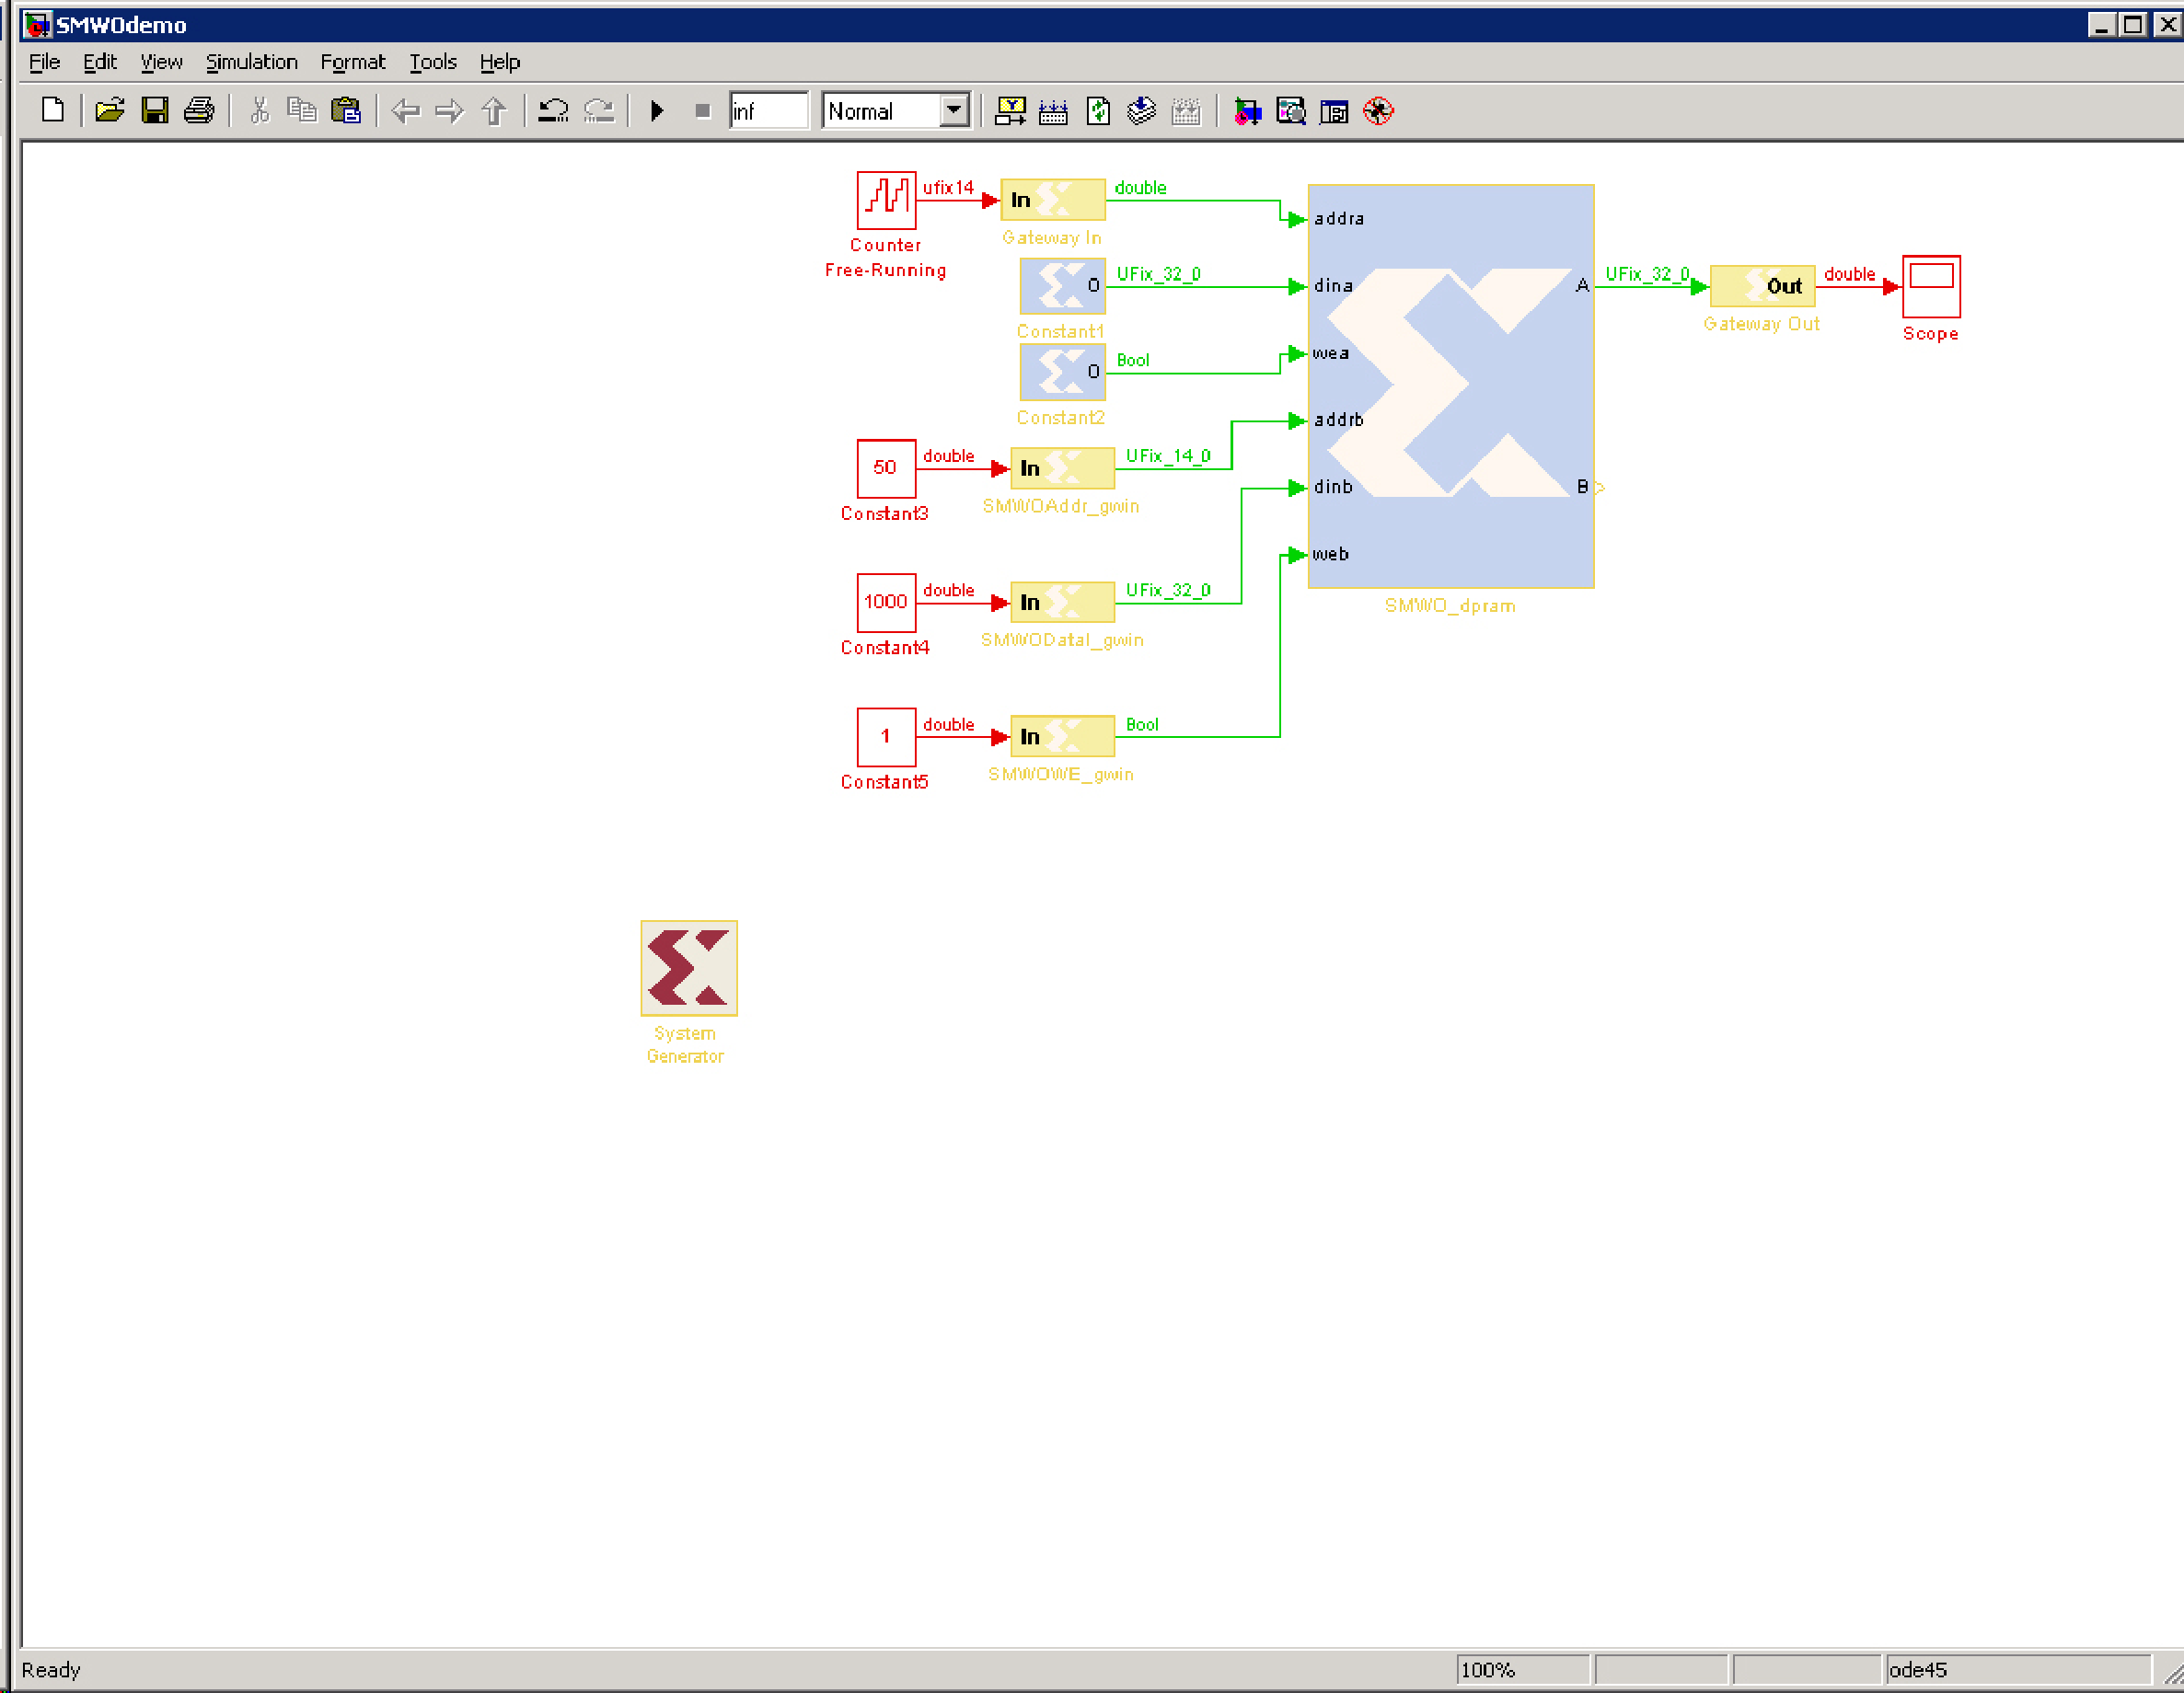
\includegraphics[width=0.70\textwidth]{SMWOdemo/UnconvertedModel.pdf}
			\caption{Unconverted Model}
			\label{fig:UnconvertedModelSMWO}
		\end{figure}
	\newpage
	\item Run the script:
	  \\sysgen2opb('SMWOdemo', hex2dec('FF000000'), 'sm')
	  	\begin{figure}[htbp]
				\centering
				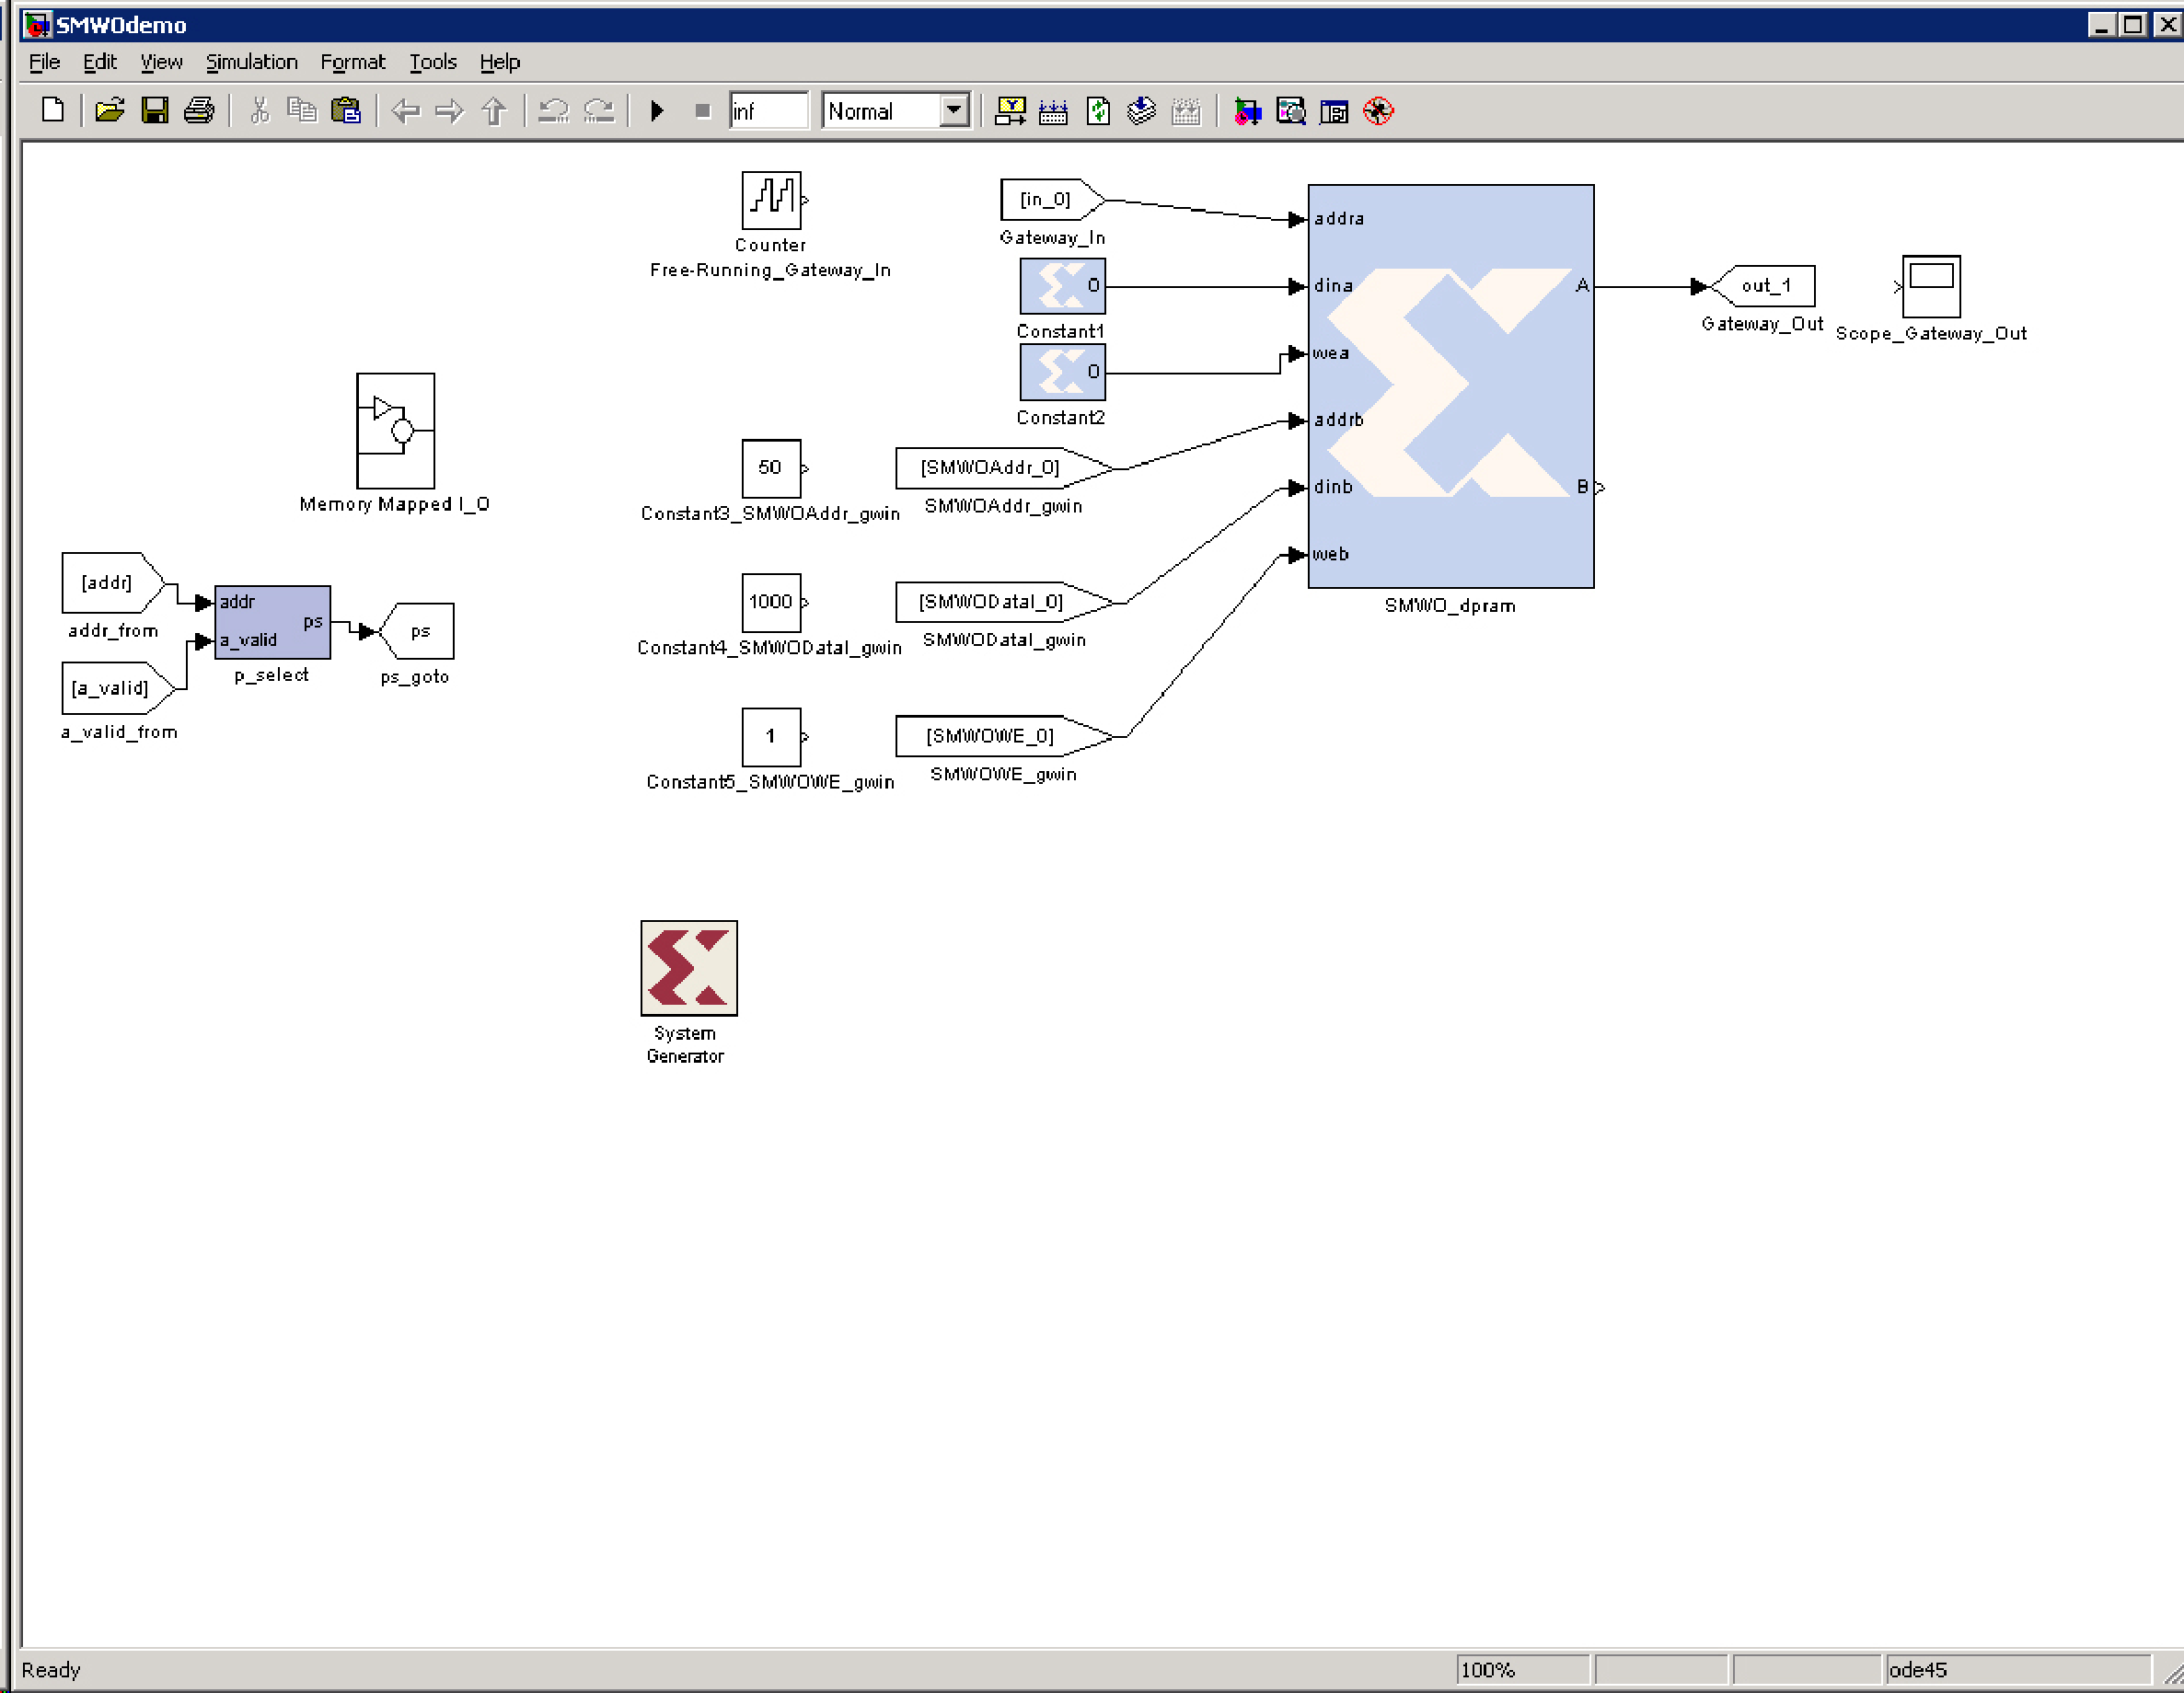
\includegraphics[width=0.70\textwidth]{SMWOdemo/ConvertedModel.pdf}
				\caption{Converted Model}
				\label{fig:ConvertedModelSMWO}
			\end{figure}
	\item Use System Generator to generate the HDL.
	
\end{enumerate}


\subsection{Xilinx Platform Studio}
\begin{enumerate}
	\item After creating the project, add the generated pcore to the XPS Project.
	\item Edit the different properties of System Assembly within XPS.
	\item Add a Software Application Project. Name the project TestSMWOdemo. Create a new C Source file. Name the file ''TestSMWOdemo.c''
	\newpage
	\item After including the necessary libraries and copying the generated .h file \\(SMWOdemo\_gatewaySMLog.h), add in the following code:
		\begin{figure}[htbp]
			\centering
			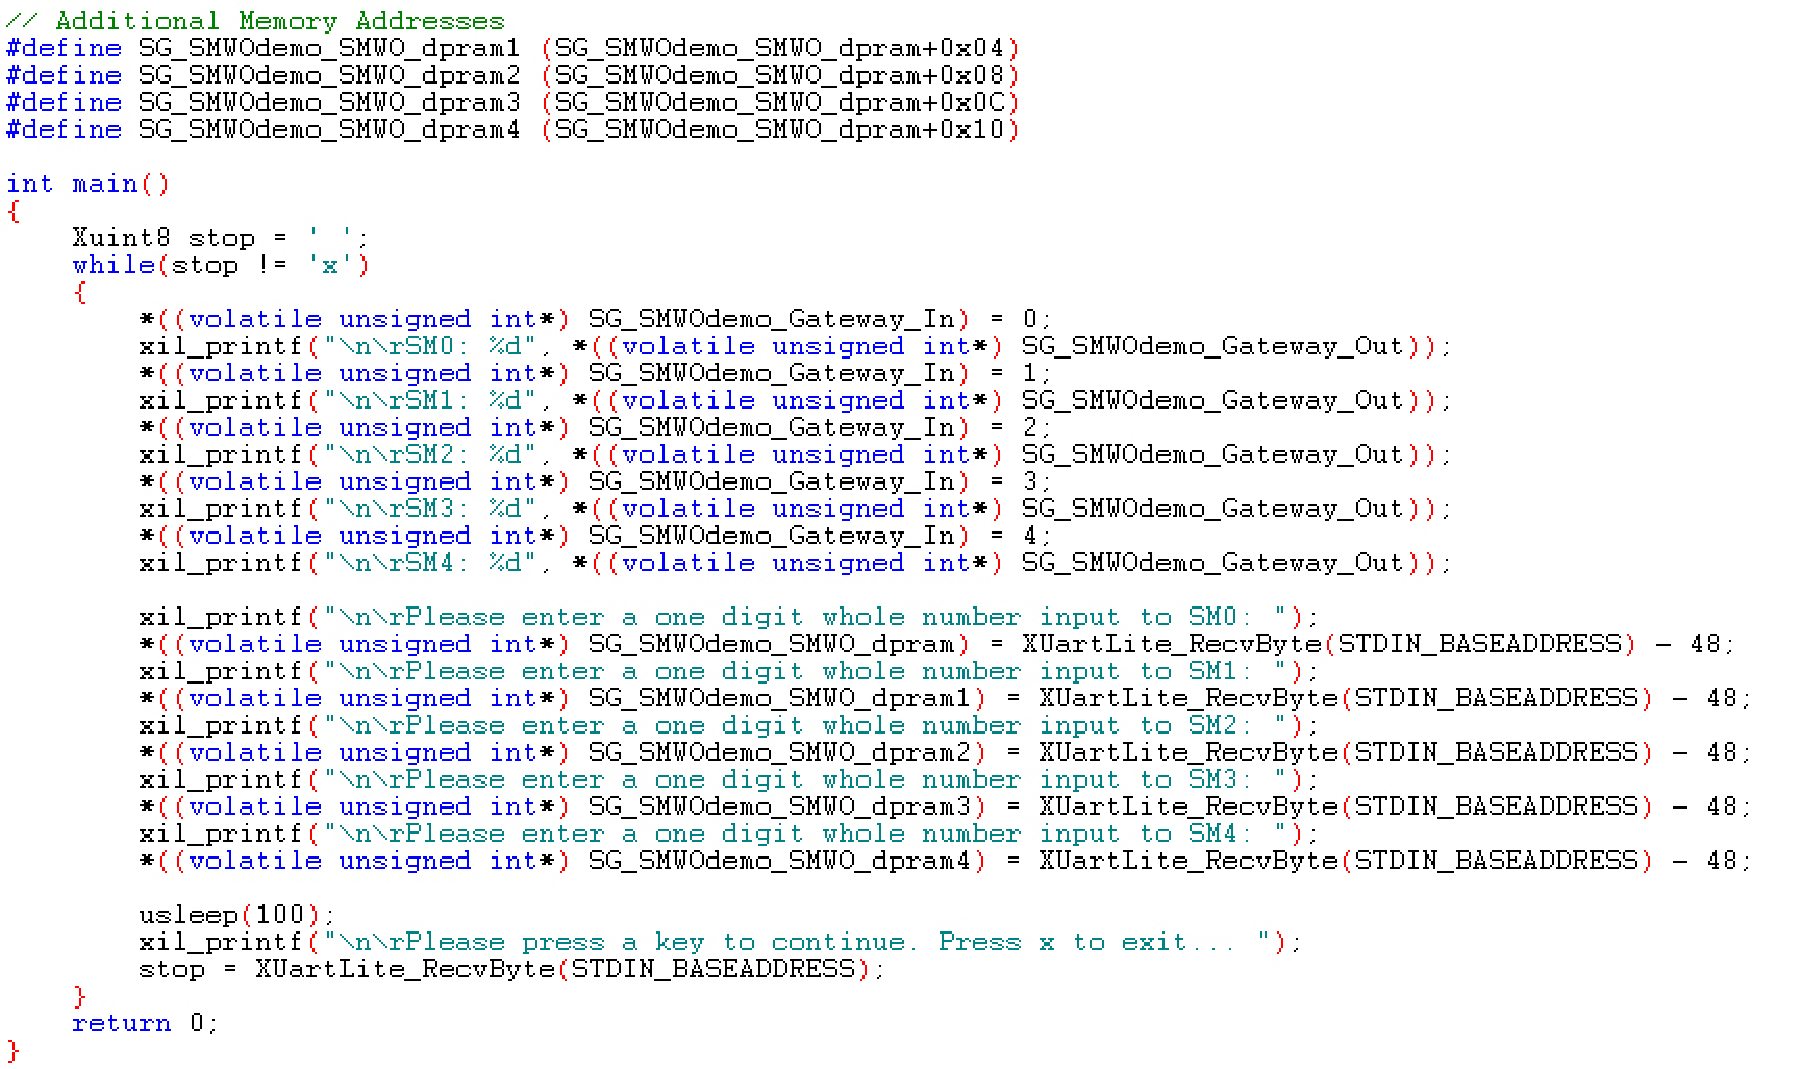
\includegraphics[width=0.90\textwidth]{SMWOdemo/code1.pdf}
			\label{fig:codeSMWO1}
		\end{figure}
	\newpage
	\item This is what the code should look like:
		\begin{figure}[htbp]
			\centering
			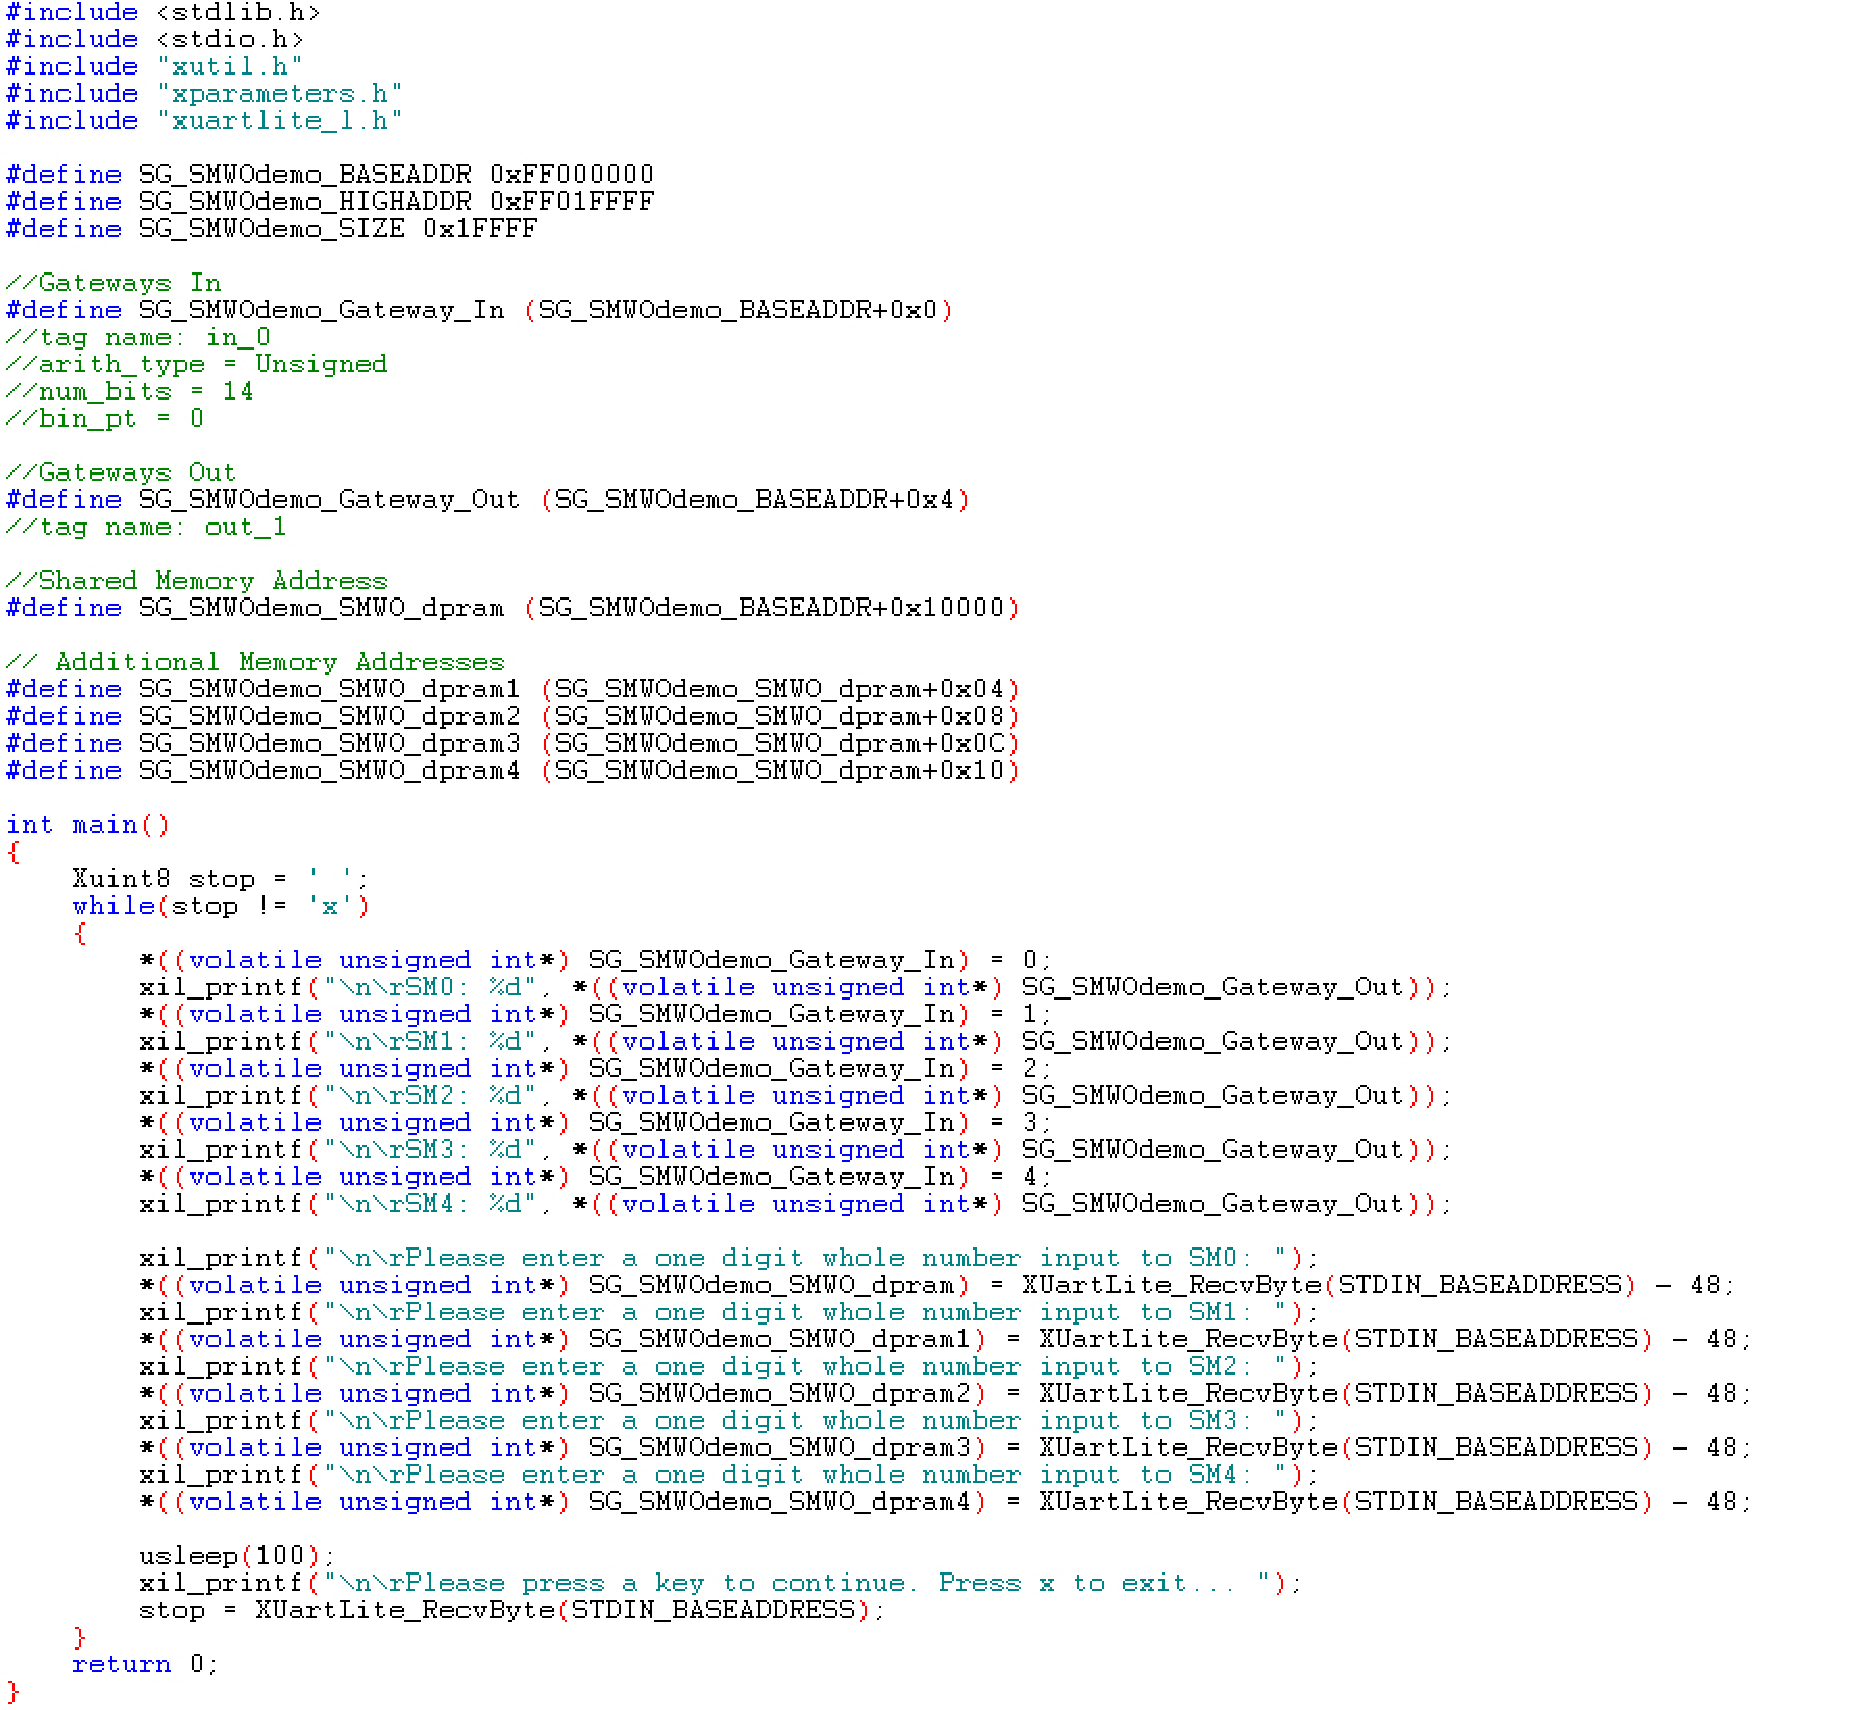
\includegraphics[width=0.90\textwidth]{SMWOdemo/code2.pdf}
			\label{fig:codeSMWO2}
		\end{figure}
	\item Save the file. Generate the bitstream. Update the bitstream. Put the bitstream onto the board and view the output.
\end{enumerate}





\newpage
\section{Example with Configurable Subsystem Extension}

\begin{enumerate}
	\item This example is exactly the same as the Example with the Original Script. However, after creating the model, run
\\\textit{sysgen2opb('adder', hex2dec('FF000000'), 'confsubsys')} in order to run the Configurable Subsystem Extension script. This is the result you should get:
	\begin{figure}[htbp]
		\centering
		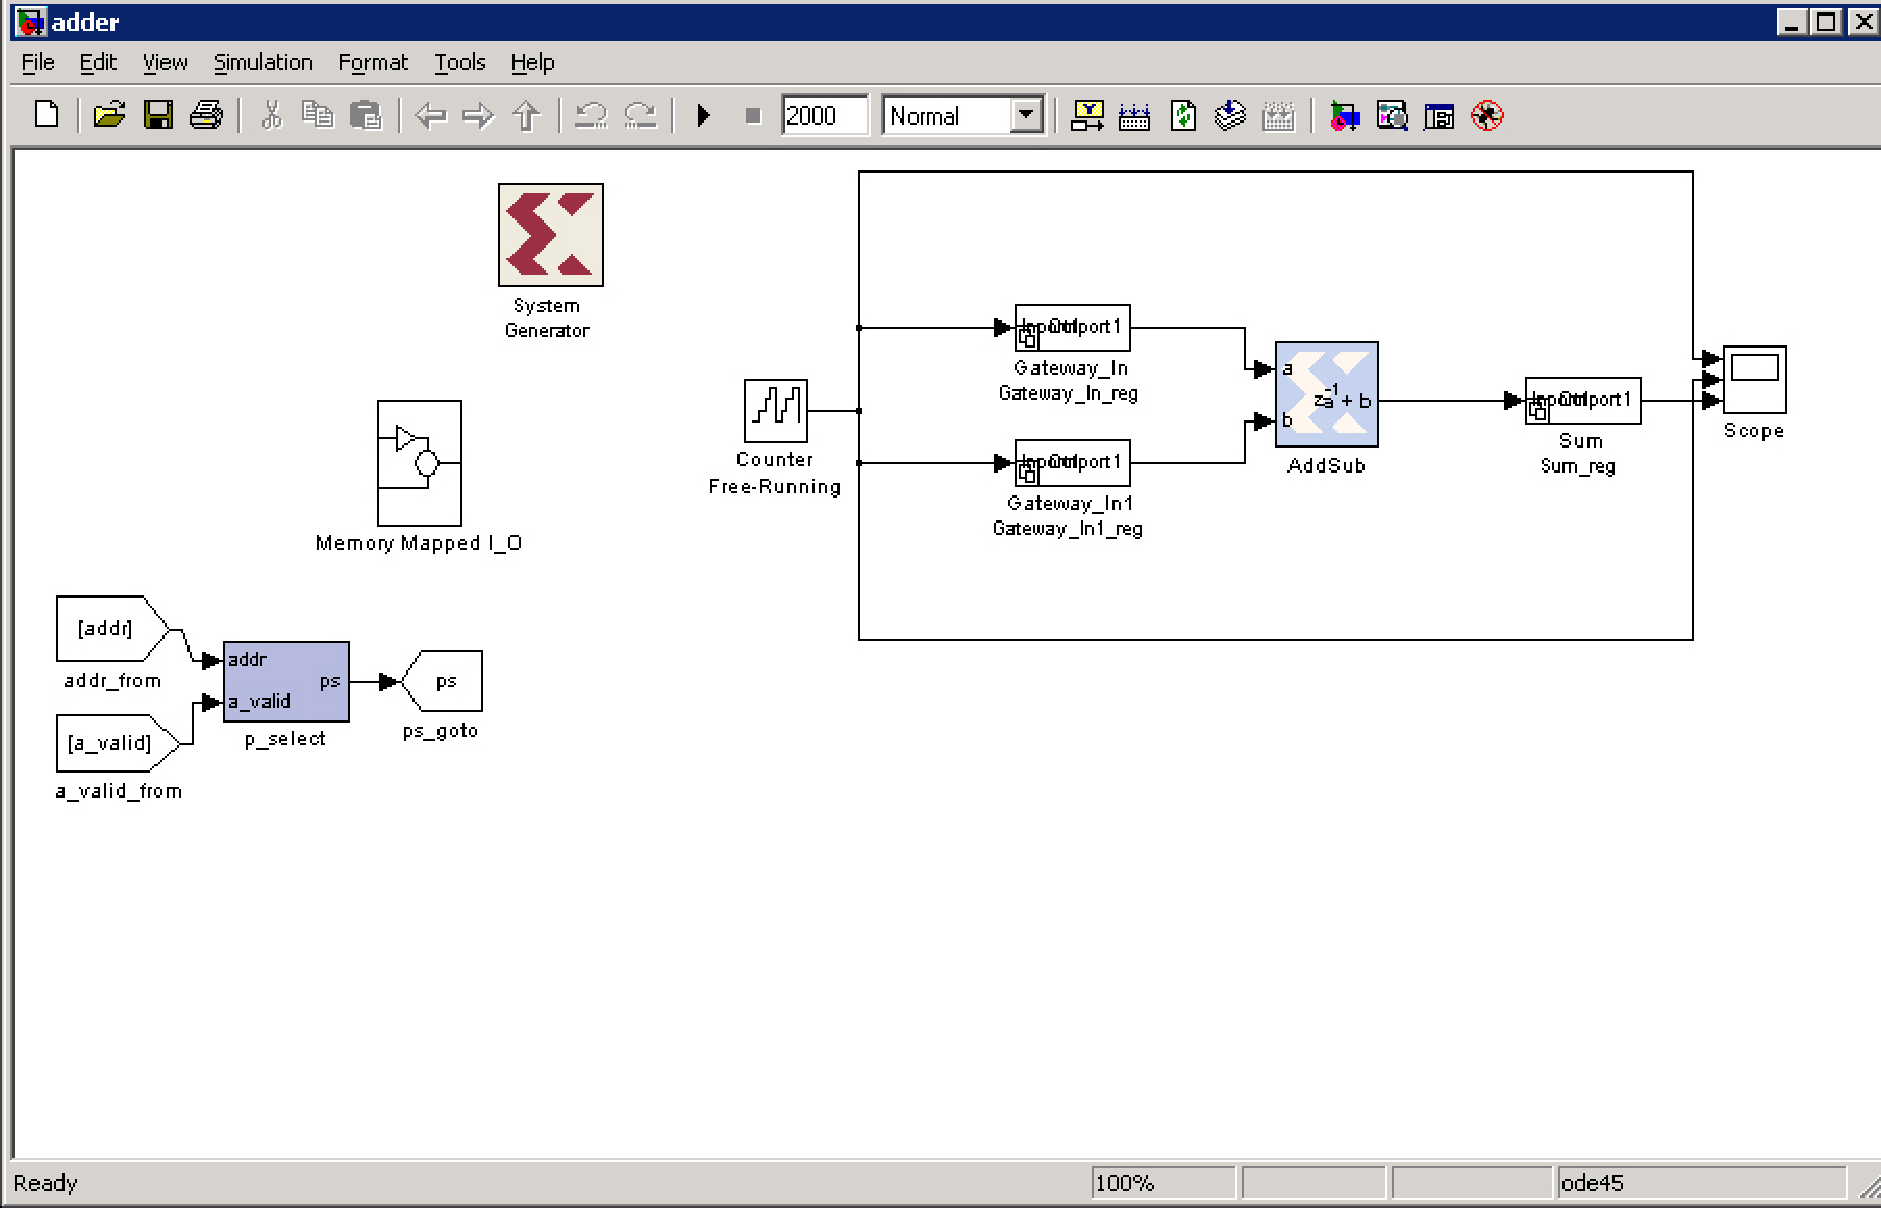
\includegraphics[width=0.50\textwidth]{CONFdemo/ConvertedModel.pdf}
		\label{fig:ConvertedModel}
	\end{figure}

	\item Now the difference is that there are configurable subsystems instead of registers. For each configurable subsystem, double-click on it. Double click on Configurable Subsystem Manager. Click on the drop-down menu and select the option that has the suffix ''\_reg.'' Click OK. Close the Configurable Subsystem Window. Make sure that you do this for all of the configurable subsystems. This will allow the OPB Export Tool to run since the Configurable Subsystem Manager selected the register option to be used in hardware generation.
	\begin{figure}[htbp]
		\centering
		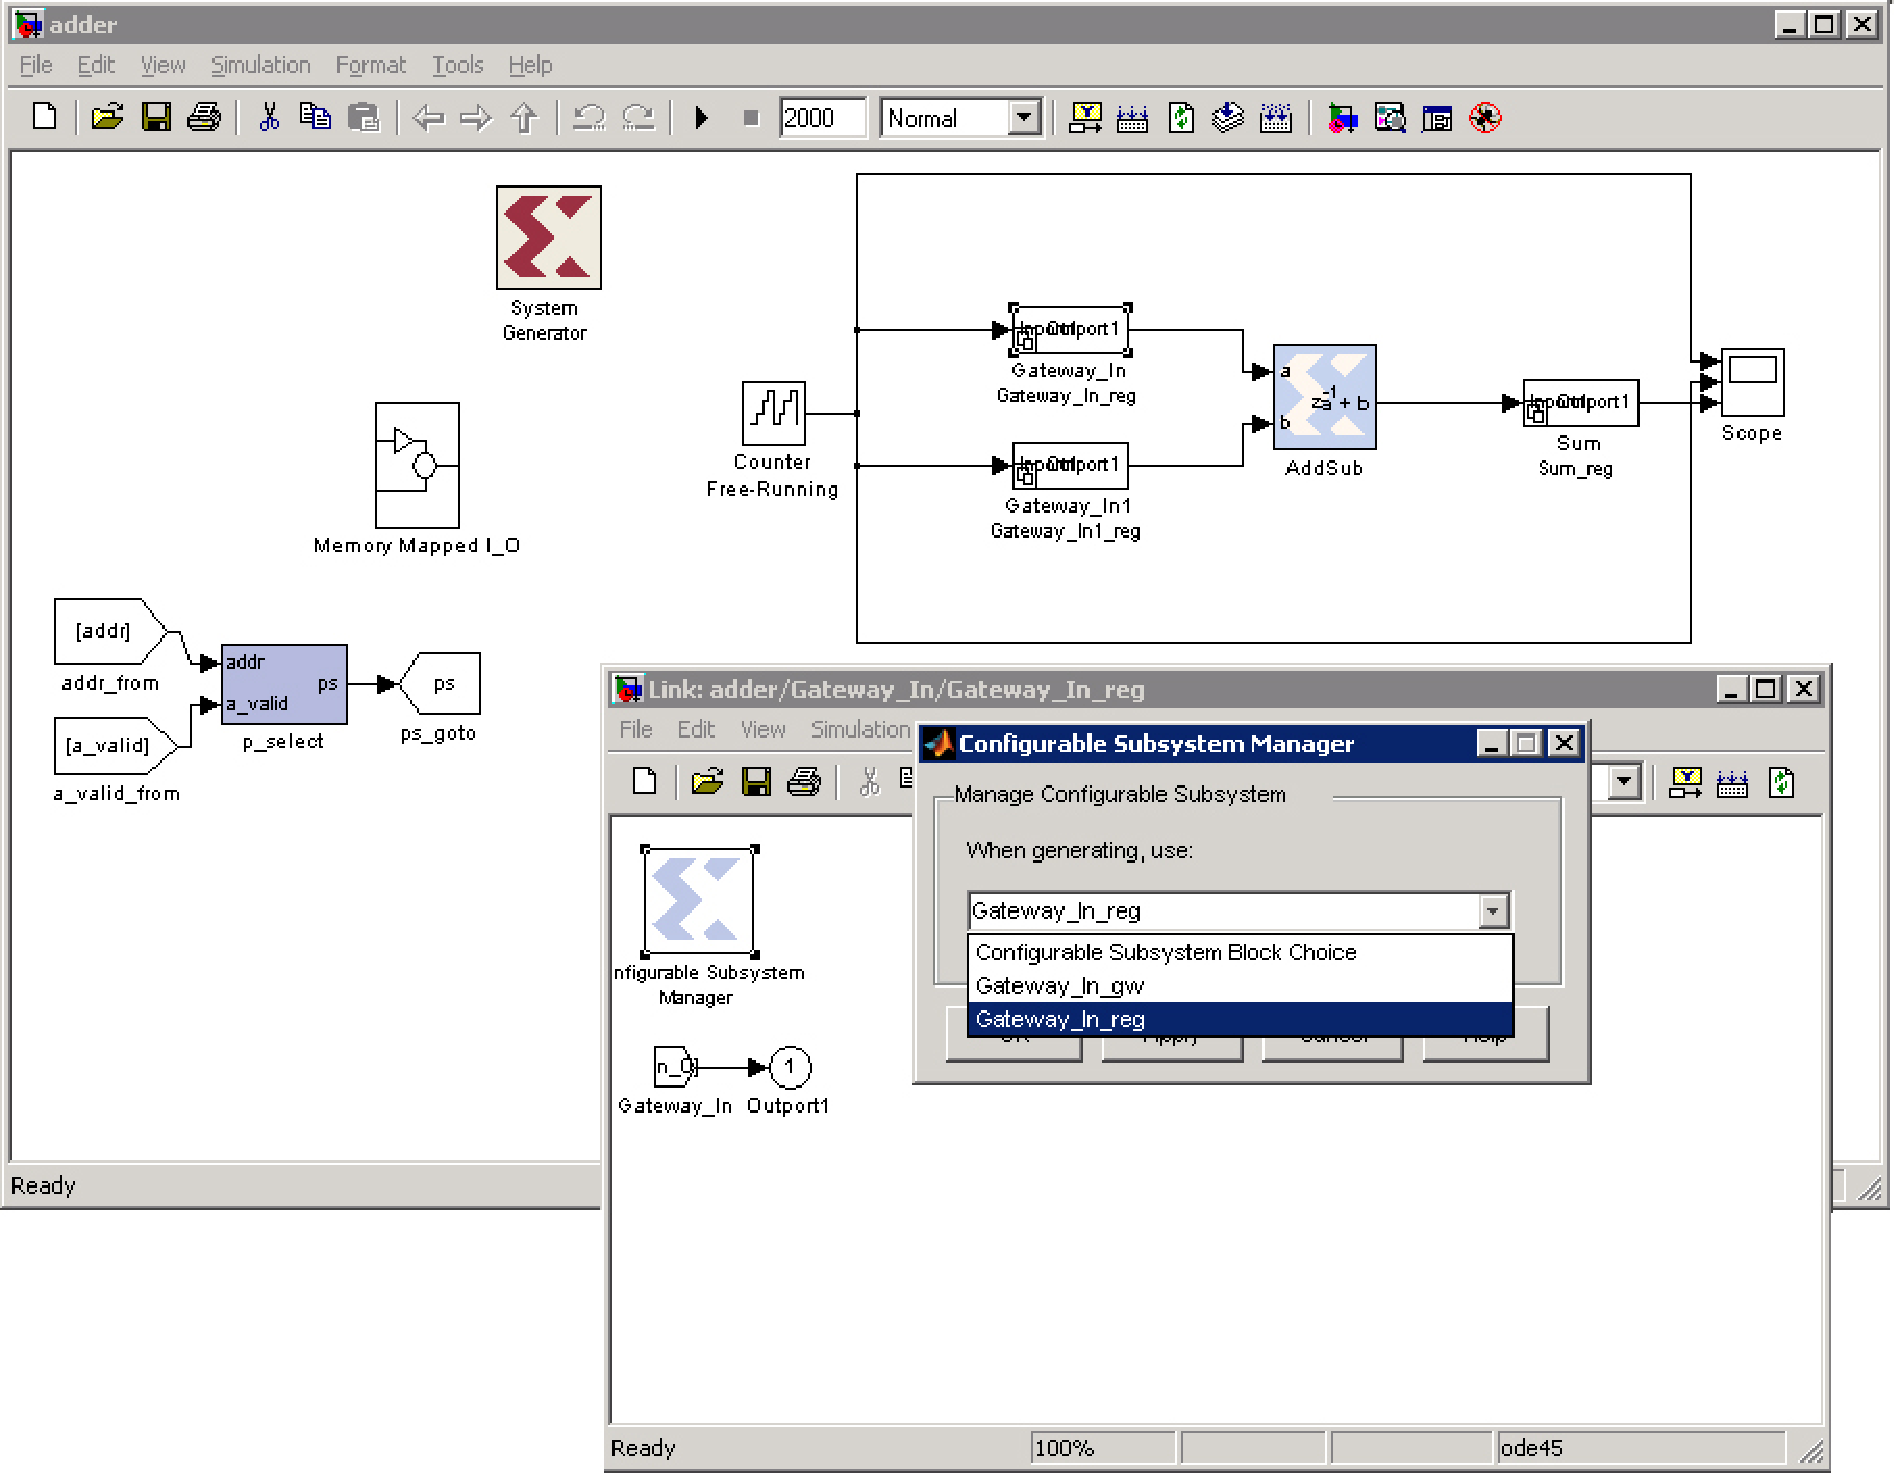
\includegraphics[width=0.50\textwidth]{CONFdemo/ConfSubsManager.pdf}
		\label{fig:ConfSubsManager}
	\end{figure}
	
	\newpage
	\item For each configurable subsystem, right-click on the configurable subsystem. Go to block choice and select the option that has the suffix ''\_gw.'' Now you can simulate the model. Also, you can still run OPB Export Tool since the Configurable Subsystem Manager has the register option selected for hardware generation.
	\begin{figure}[htbp]
		\centering
		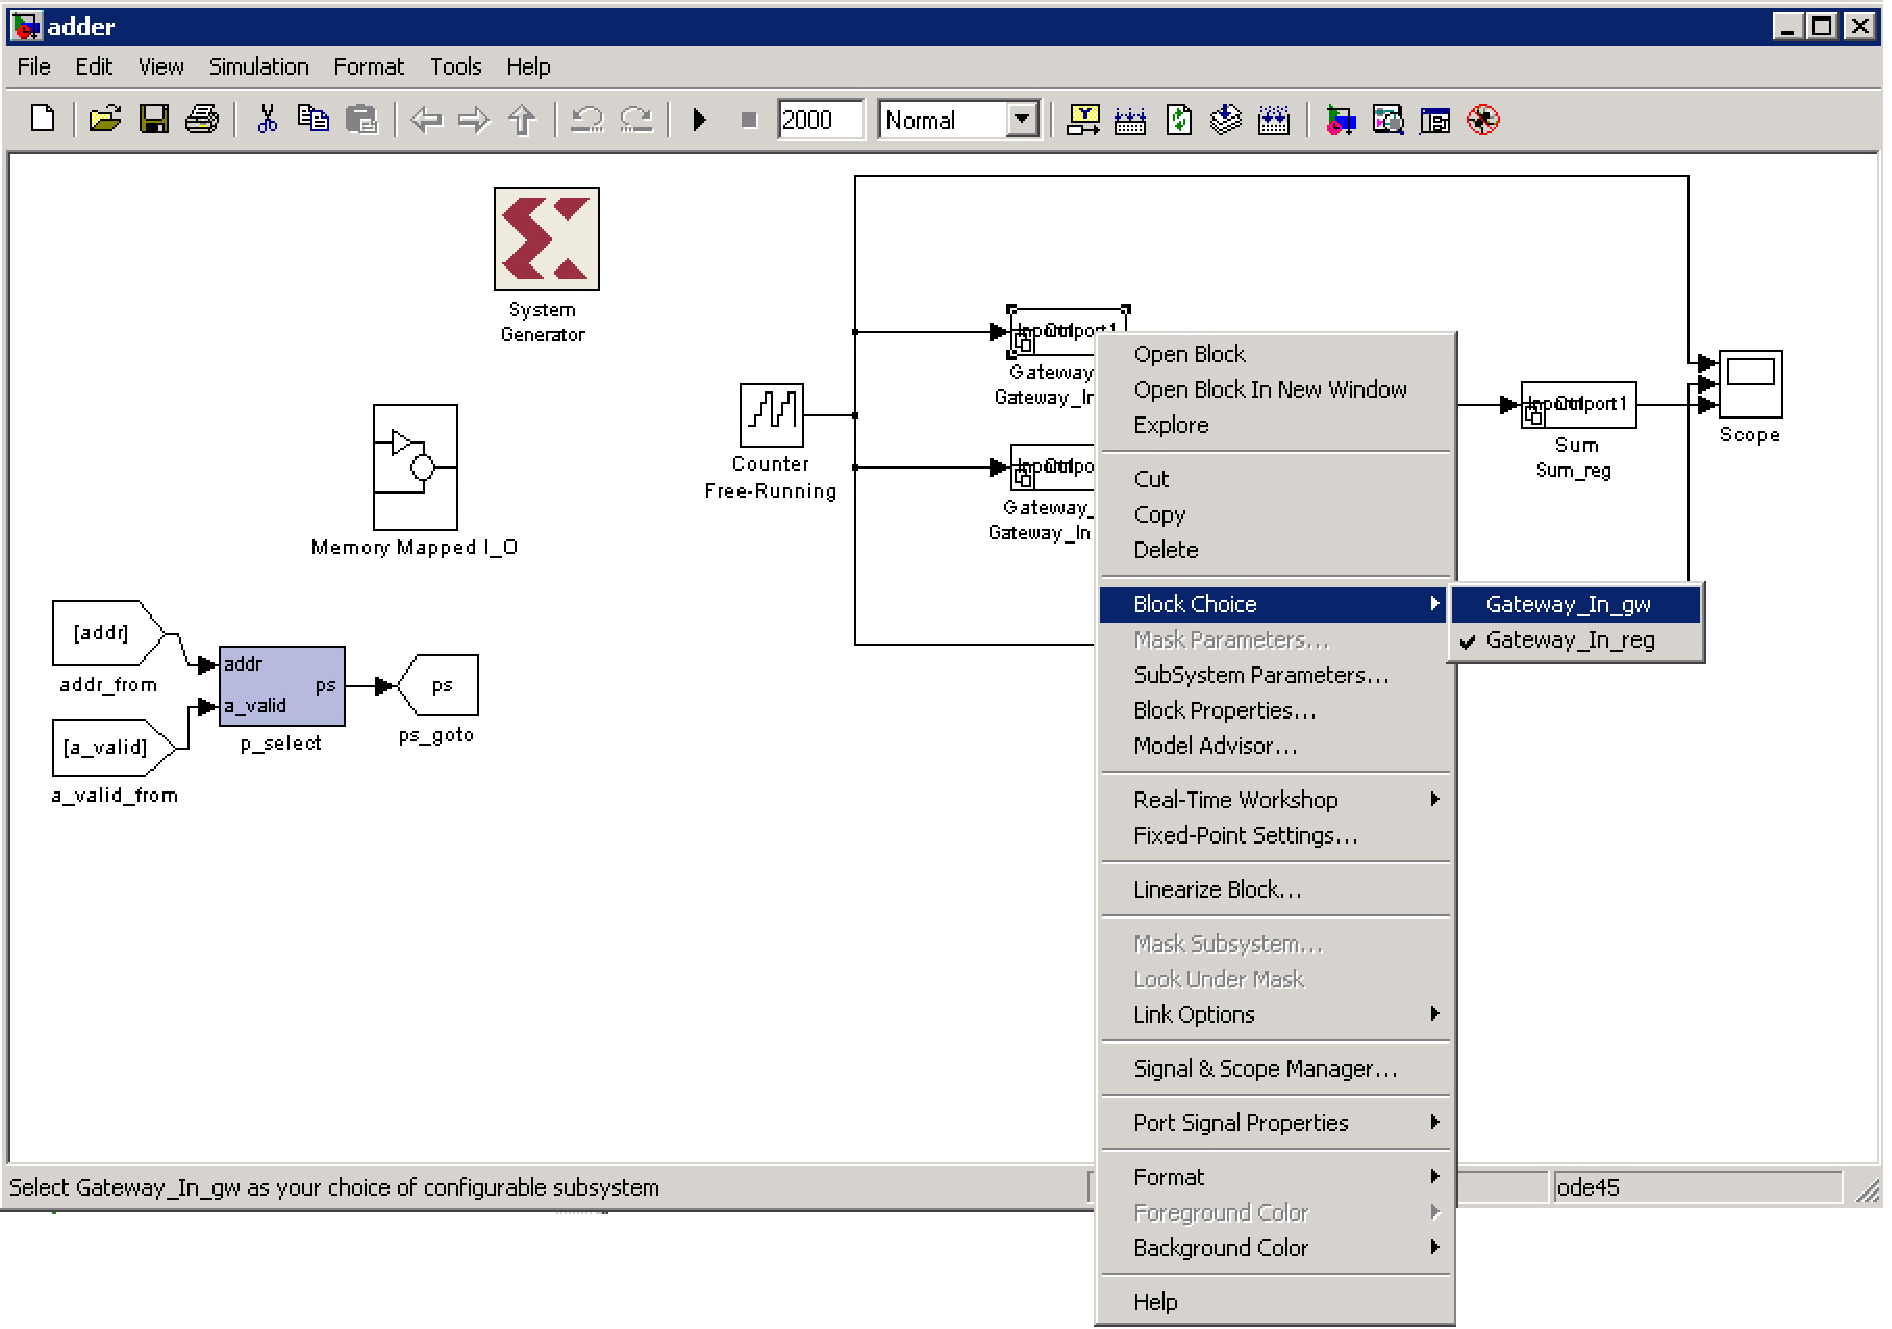
\includegraphics[width=0.50\textwidth]{CONFdemo/BlockChoice.pdf}
		\label{fig:BlockChoice}
	\end{figure}

\end{enumerate}





\newpage
\section{Sysgen2OPB : Syntax and Usage}
This section briefly describes the syntax and usage of the sysgen2opb script.

\begin{enumerate}
	\item The syntax for the script in the Matlab command window is: 
		\\\textit{sysgen2opb('YourModelName', hex2dec('YourBaseAddr'), 'YourSelection', 'YourPrefix')}
		\begin{enumerate}
			\item Replace 'YourModelName' with your Simulink/System Generator model's name without the .mdl extension.
			\item Replace 'YourBaseAddr' with a 32-bit memory address in hexidecimal notation. \\FF100000 is usually a safe choice.
			\item Replace 'YourSelection' with one of the following:
				\begin{enumerate}
					\item 'orig' which will run the Simple Registers Script
					\item 'sm' which will run the Shared Memory Extension Script
					\item 'confsubsys' which will run the Configurable Subsystem Extension Script
				\end{enumerate}
			\item Replace 'YourPrefix' with a string which will replace the ''no\_reg\_'' prefix attached to unconverted gateways. Use a blank string ('') to simply strip the ''no\_reg\_'' prefix. 
			\item There are two defaults in the script
				\begin{enumerate}
					\item If you want to run the Simple Registers Script with a blank string to strip away the ''no\_reg\_'' prefix, run:
     						\\sysgen2opb('yourModelName', hex2dec('yourBaseAddress'))
 					
 					\item If you want to run one of the scripts with a blank strip to strip away the ''no\_reg\_'' prefix, run:
     						\\sysgen2opb('yourModelName', hex2dec('yourBaseAddress'), 'yourSelection')
				\end{enumerate}

	\end{enumerate}
\end{enumerate}

\end{document}